%%%%%%%%%%%%%%%%%%%%%%%%%%%%%%%%%%%%%%%%%%%%%%%%%%%%%%%%%%%%%%%%%%%%%%%%%%%%%%%%%%
\begin{frame}[fragile]\frametitle{}
\begin{center}
{\Large Background}\\

{till word2vec}

\end{center}
\end{frame}



%%%%%%%%%%%%%%%%%%%%%%%%%%%%%%%%%%%%%%%%%%%%%%%%%%%%%%%%%%%
\begin{frame}[fragile]\frametitle{How do we represent the meaning of a word?}
Definition: meaning (Webster dictionary)

\begin{itemize}
\item the idea that is represented by a word, phrase, etc.
\item the idea that a person wants to express by using  words, signs, etc.
\item the idea that is expressed in a work of writing, art, etc.  
\end{itemize}

Commonest linguistic way of thinking of meaning:

\begin{center}
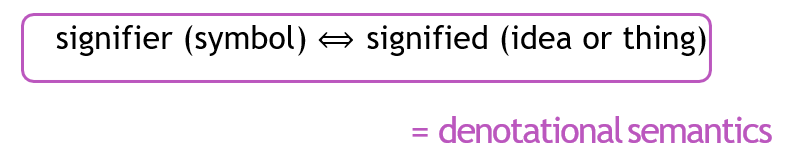
\includegraphics[width=0.6\linewidth,keepaspectratio]{bert2}
\end{center}		  

{\tiny (Ref: CS224n: Natural Language Processing with Deep Learning - Christopher Manning)}

\end{frame}


%%%%%%%%%%%%%%%%%%%%%%%%%%%%%%%%%%%%%%%%%%%%%%%%%%%%%%%%%%%
\begin{frame}[fragile]\frametitle{How do we have usable meaning in a computer?}


\begin{center}
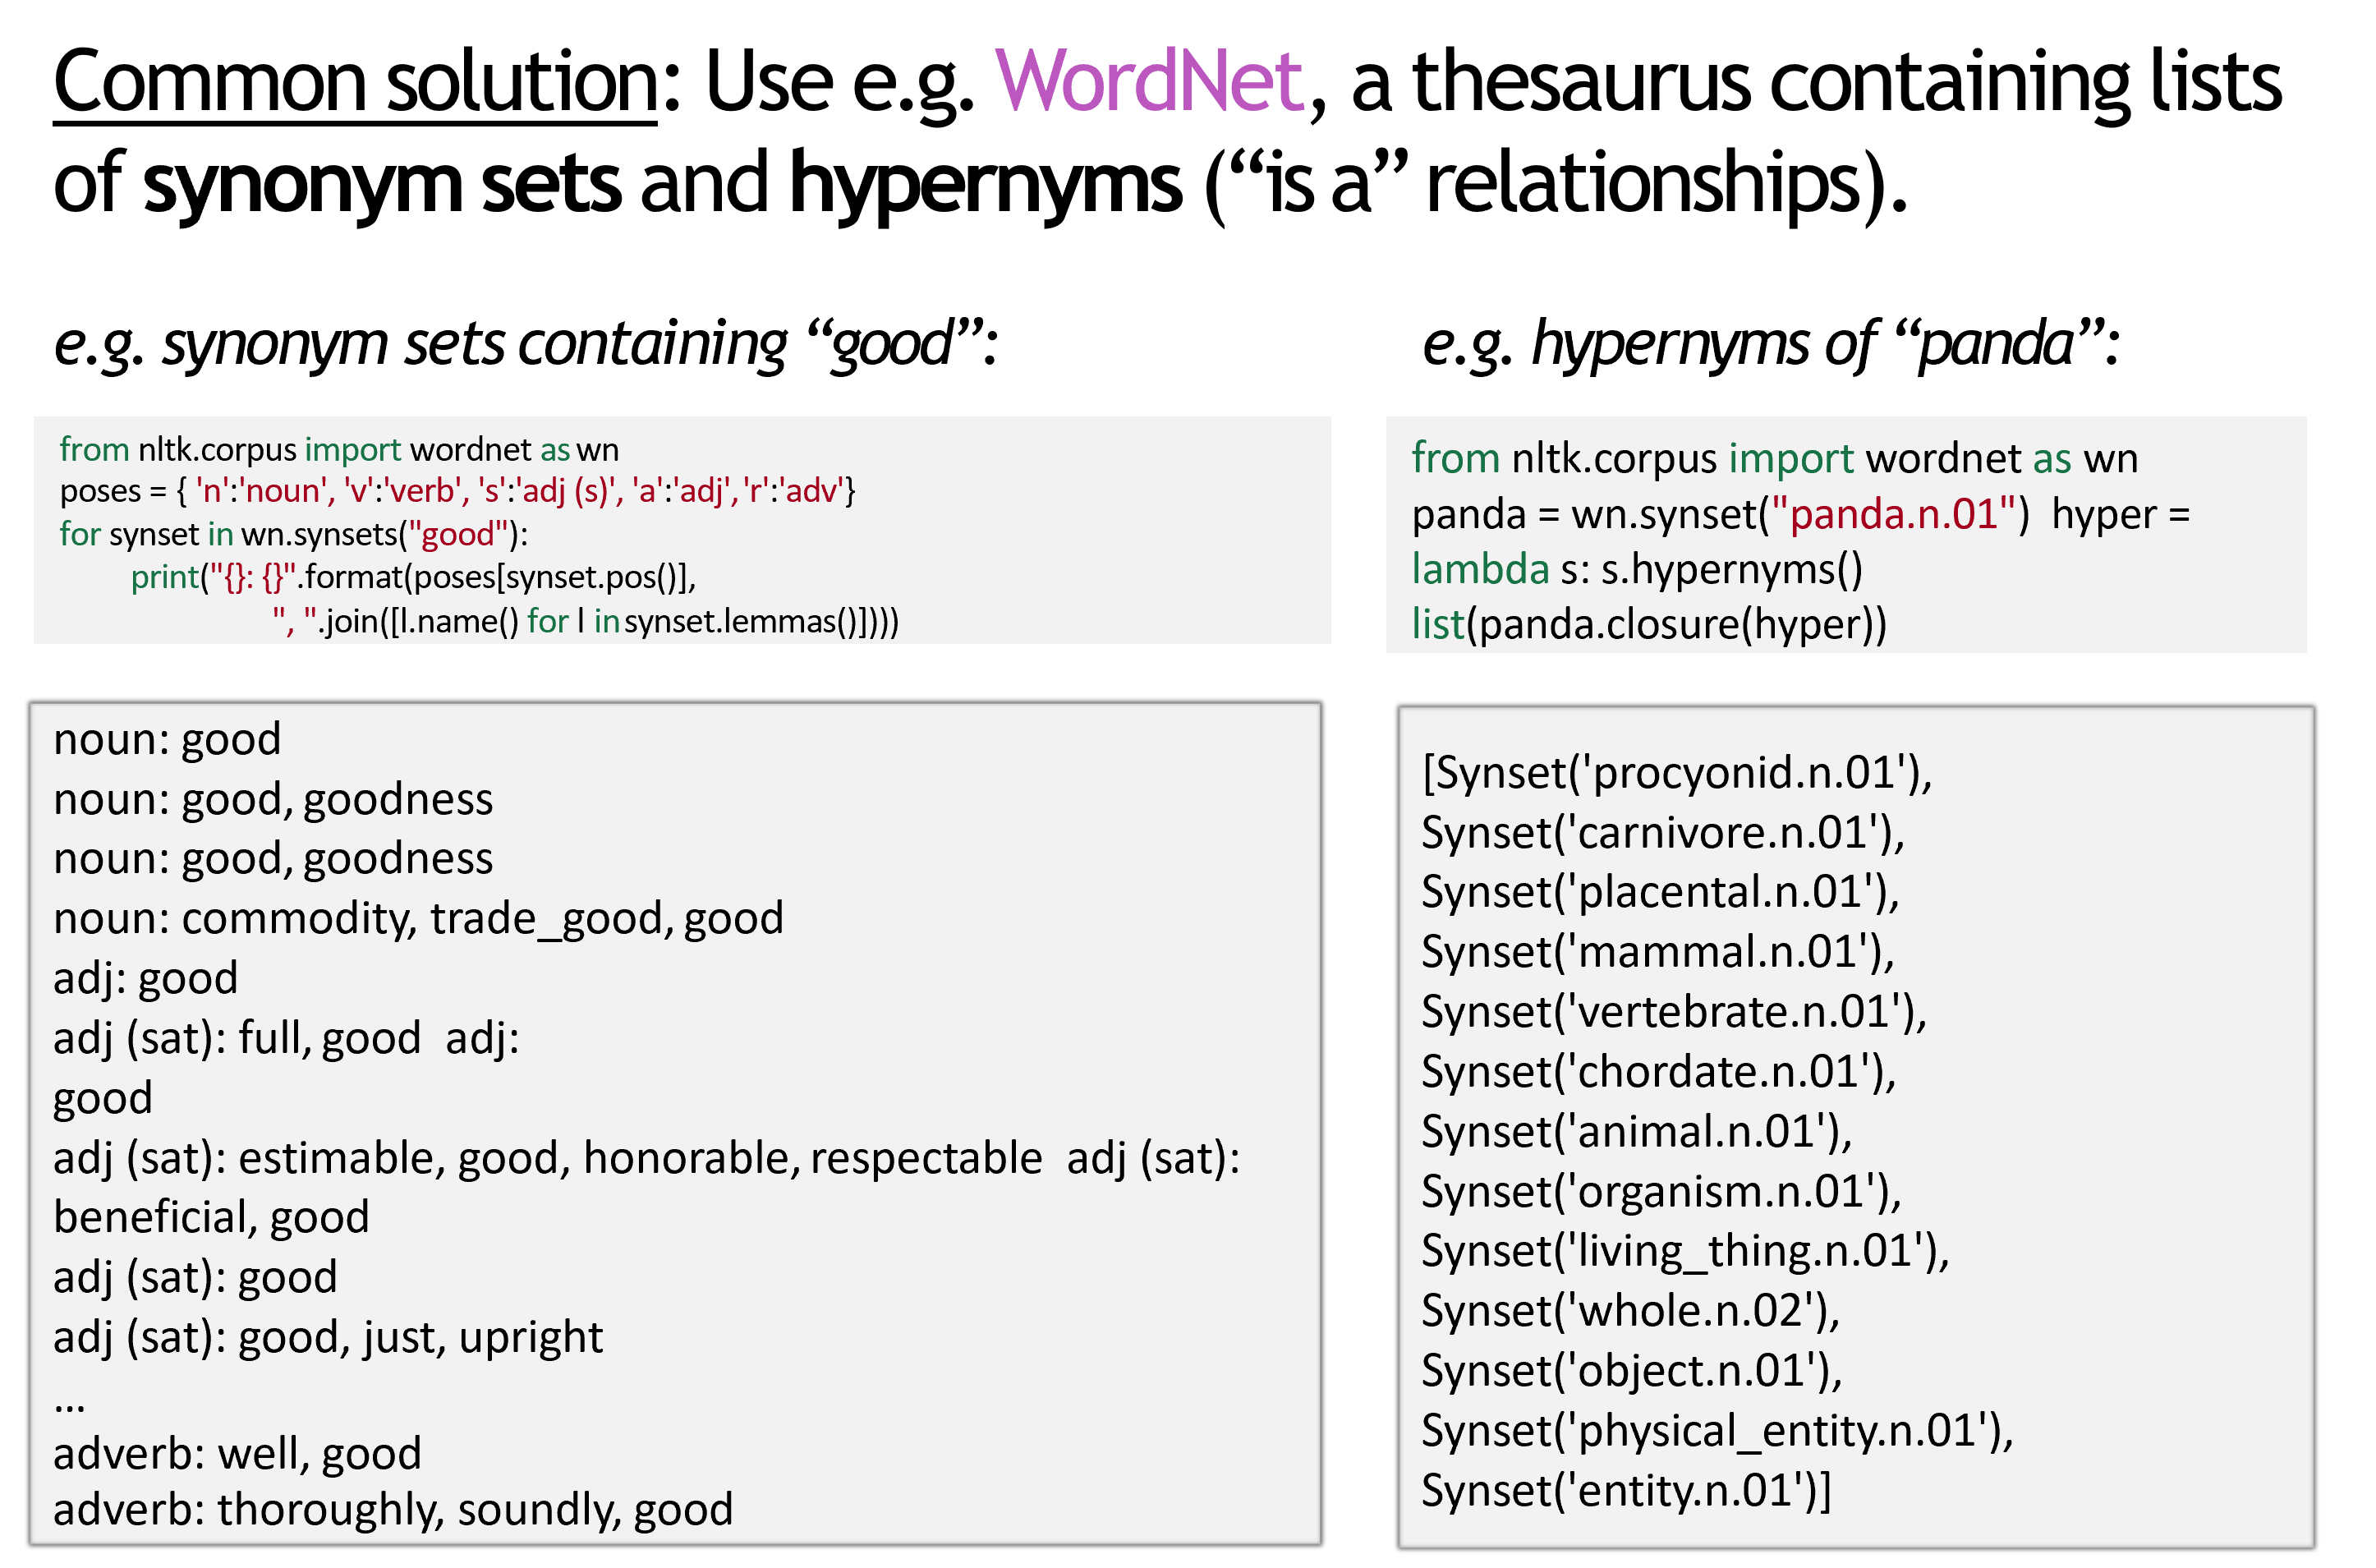
\includegraphics[width=\linewidth,keepaspectratio]{bert3}
\end{center}		  

{\tiny (Ref: CS224n: Natural Language Processing with Deep Learning - Christopher Manning)}

\end{frame}

%%%%%%%%%%%%%%%%%%%%%%%%%%%%%%%%%%%%%%%%%%%%%%%%%%%%%%%%%%%
\begin{frame}[fragile]\frametitle{Problems with resources like WordNet}


\begin{itemize}
\item Great as a resource but missing nuance: e.g. ``proficient'' is listed as a synonym for ``good''.  This is only correct in some contexts.
\item Missing new meanings of words: e.g., wicked, badass, nifty, wizard, genius, ninja, bombest. Impossible to keep up-to-date!
\item Subjective
\item Requires human labor to create and adapt
\item Can't compute accurate word similarity 
\end{itemize}

{\tiny (Ref: CS224n: Natural Language Processing with Deep Learning - Christopher Manning)}

\end{frame}

%%%%%%%%%%%%%%%%%%%%%%%%%%%%%%%%%%%%%%%%%%%%%%%%%%%%%%%%%%%
\begin{frame}[fragile]\frametitle{Representing words as discrete symbols}


\begin{center}
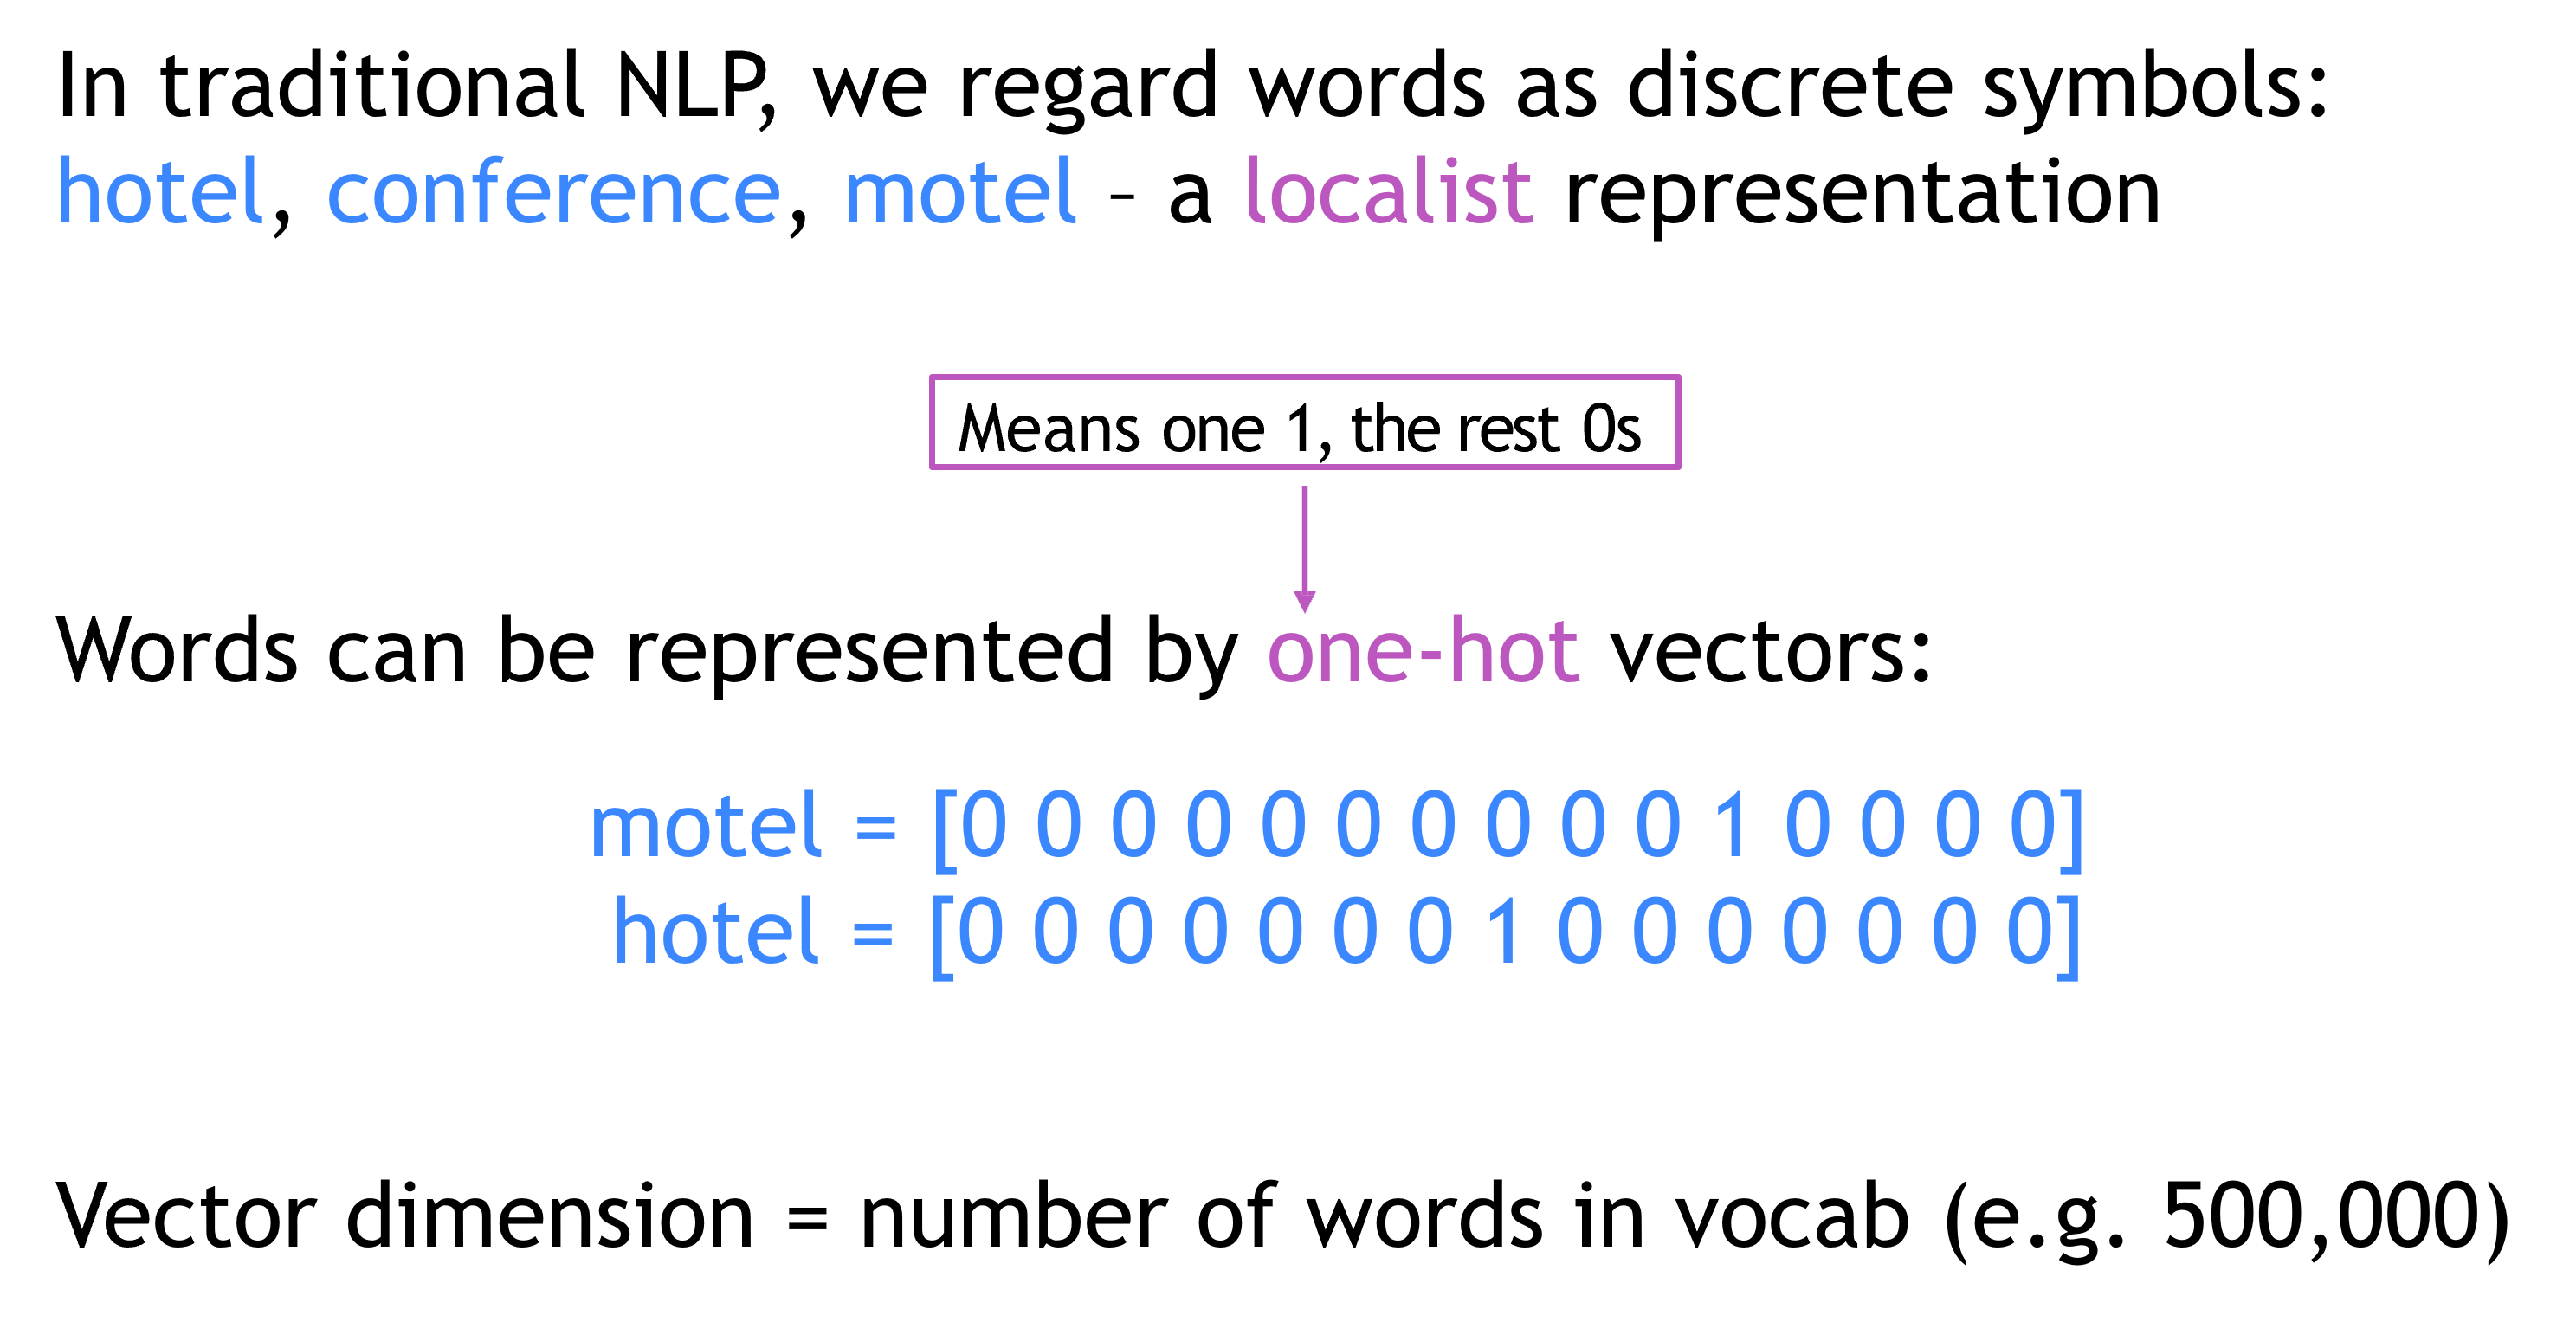
\includegraphics[width=\linewidth,keepaspectratio]{bert4}
\end{center}		  


{\tiny (Ref: CS224n: Natural Language Processing with Deep Learning - Christopher Manning)}

\end{frame}

%%%%%%%%%%%%%%%%%%%%%%%%%%%%%%%%%%%%%%%%%%%%%%%%%%%%%%%%%%%
\begin{frame}[fragile]\frametitle{Representing words as discrete symbols}


\begin{center}
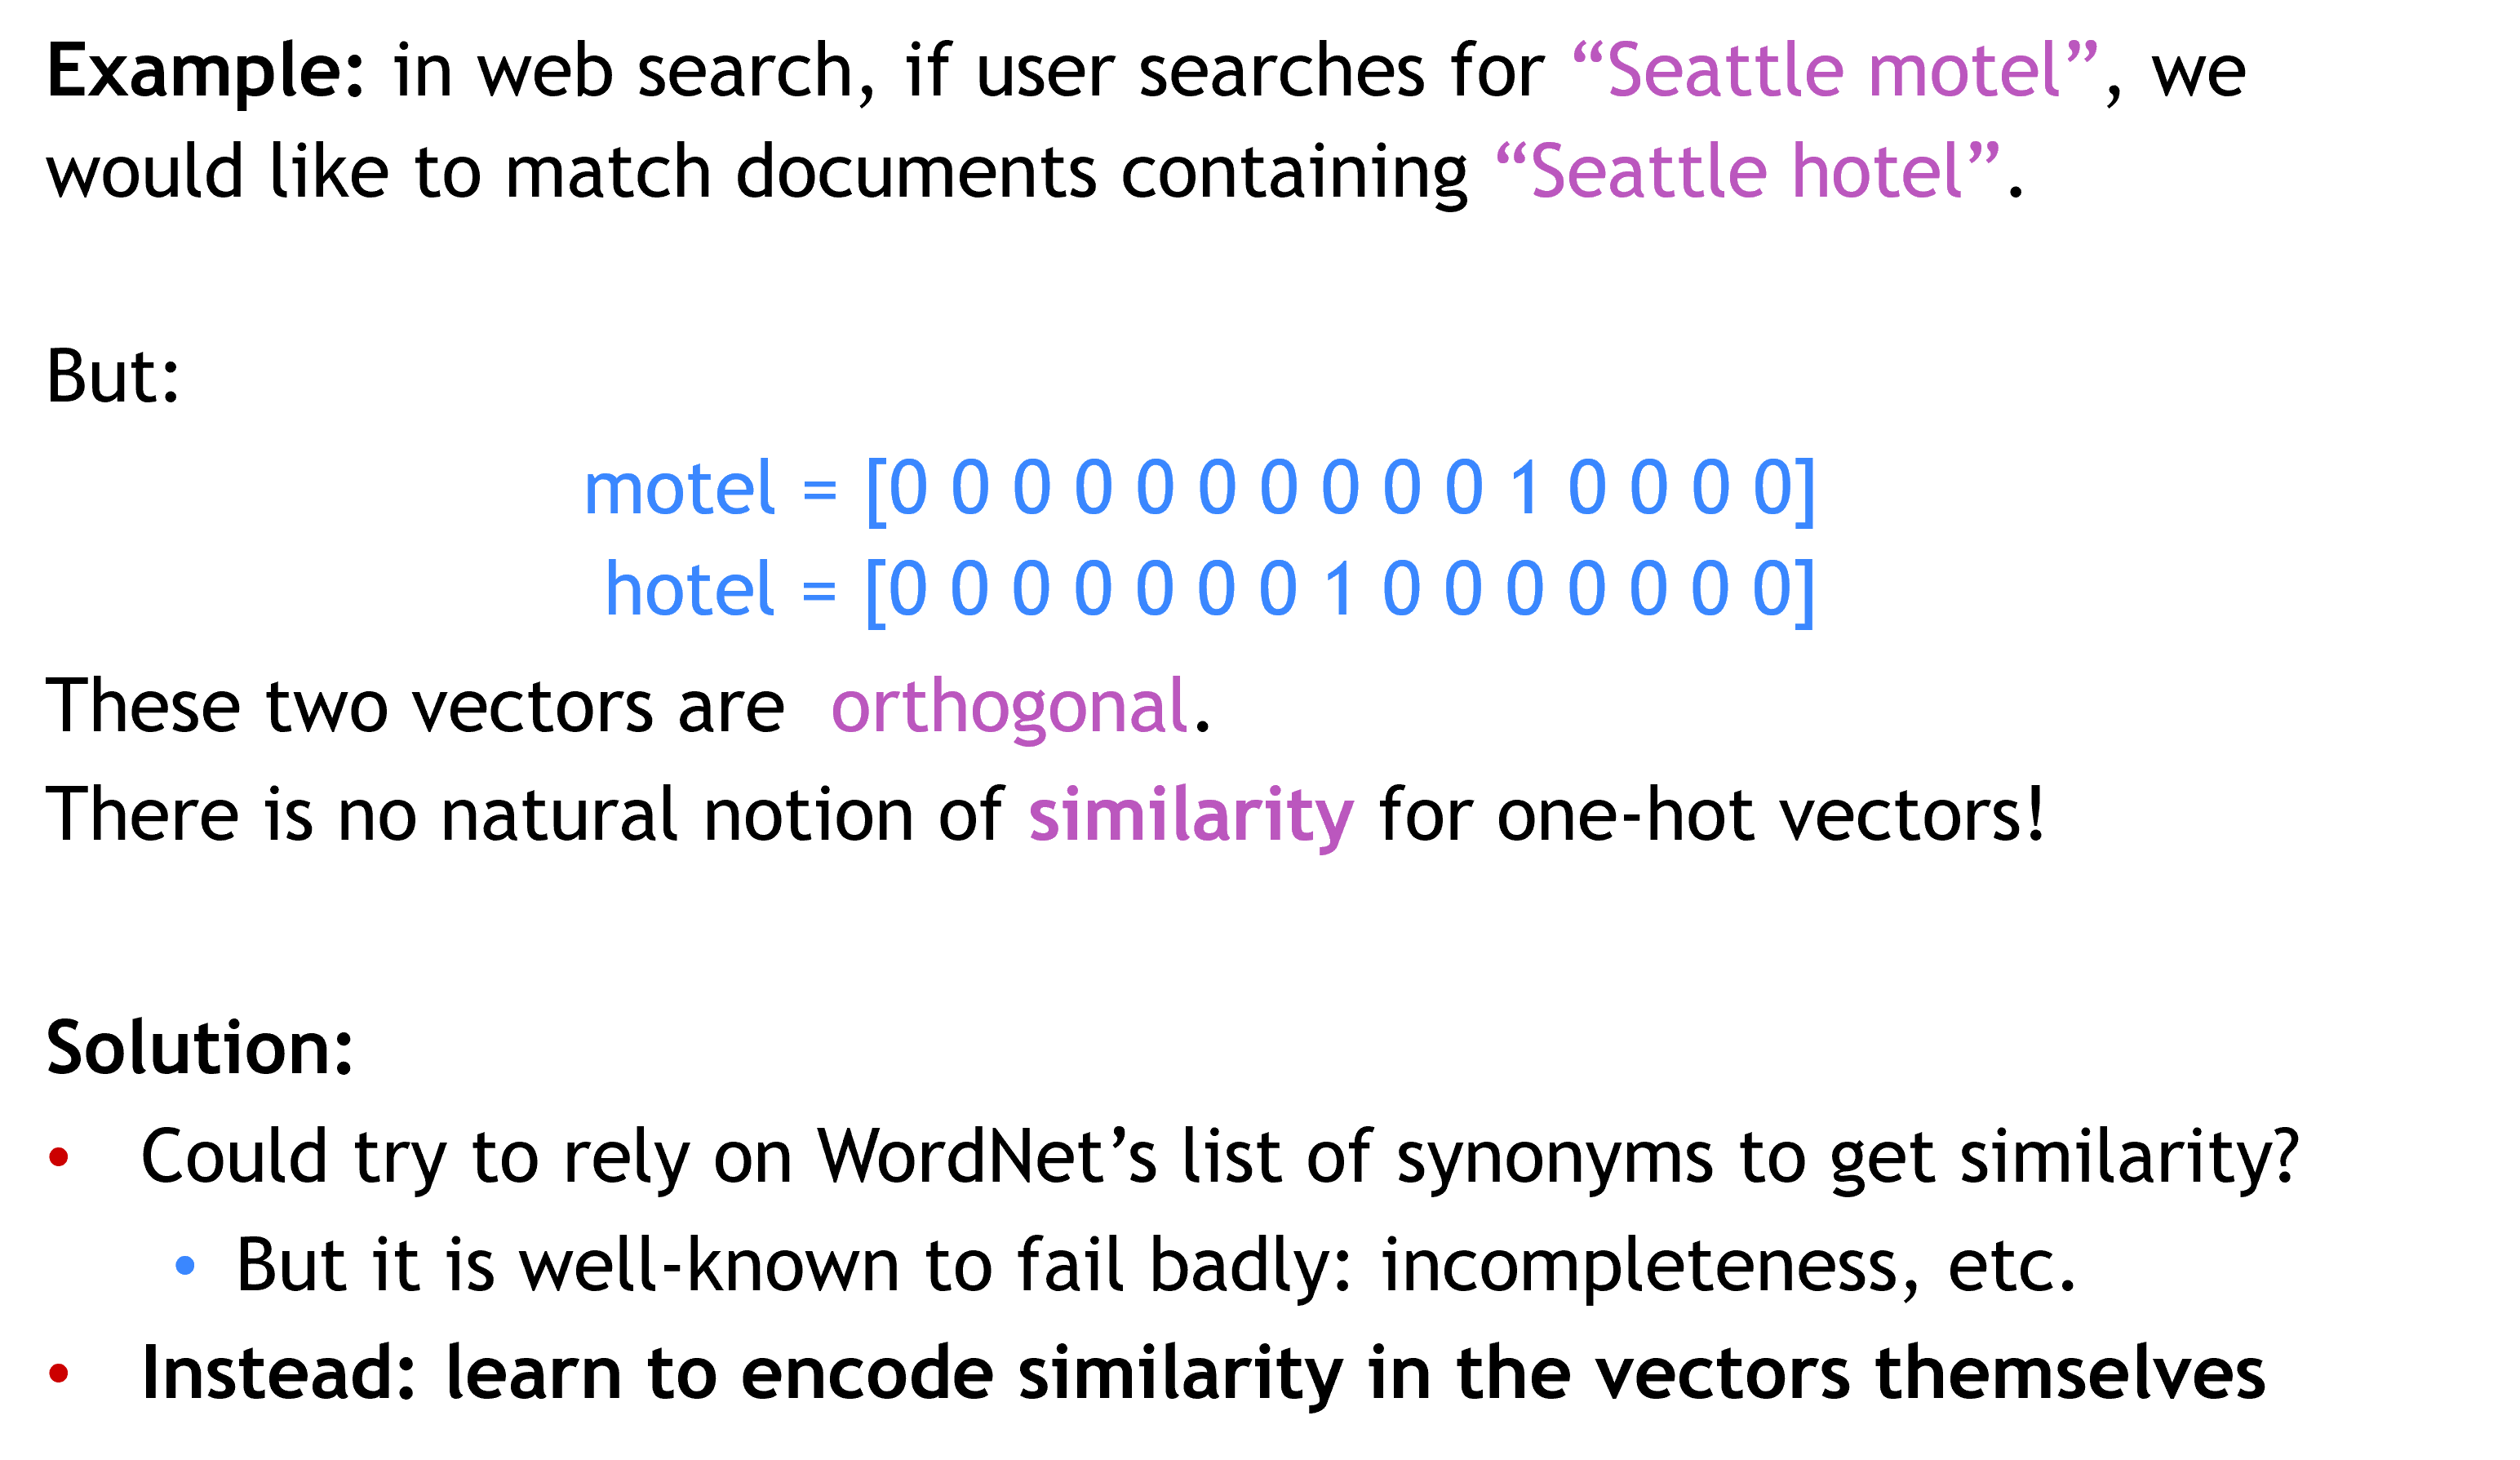
\includegraphics[width=\linewidth,keepaspectratio]{bert5}
\end{center}		  


{\tiny (Ref: CS224n: Natural Language Processing with Deep Learning - Christopher Manning)}

\end{frame}

%%%%%%%%%%%%%%%%%%%%%%%%%%%%%%%%%%%%%%%%%%%%%%%%%%%%%%%%%%%
\begin{frame}[fragile]\frametitle{Representing words by their context}


\begin{center}
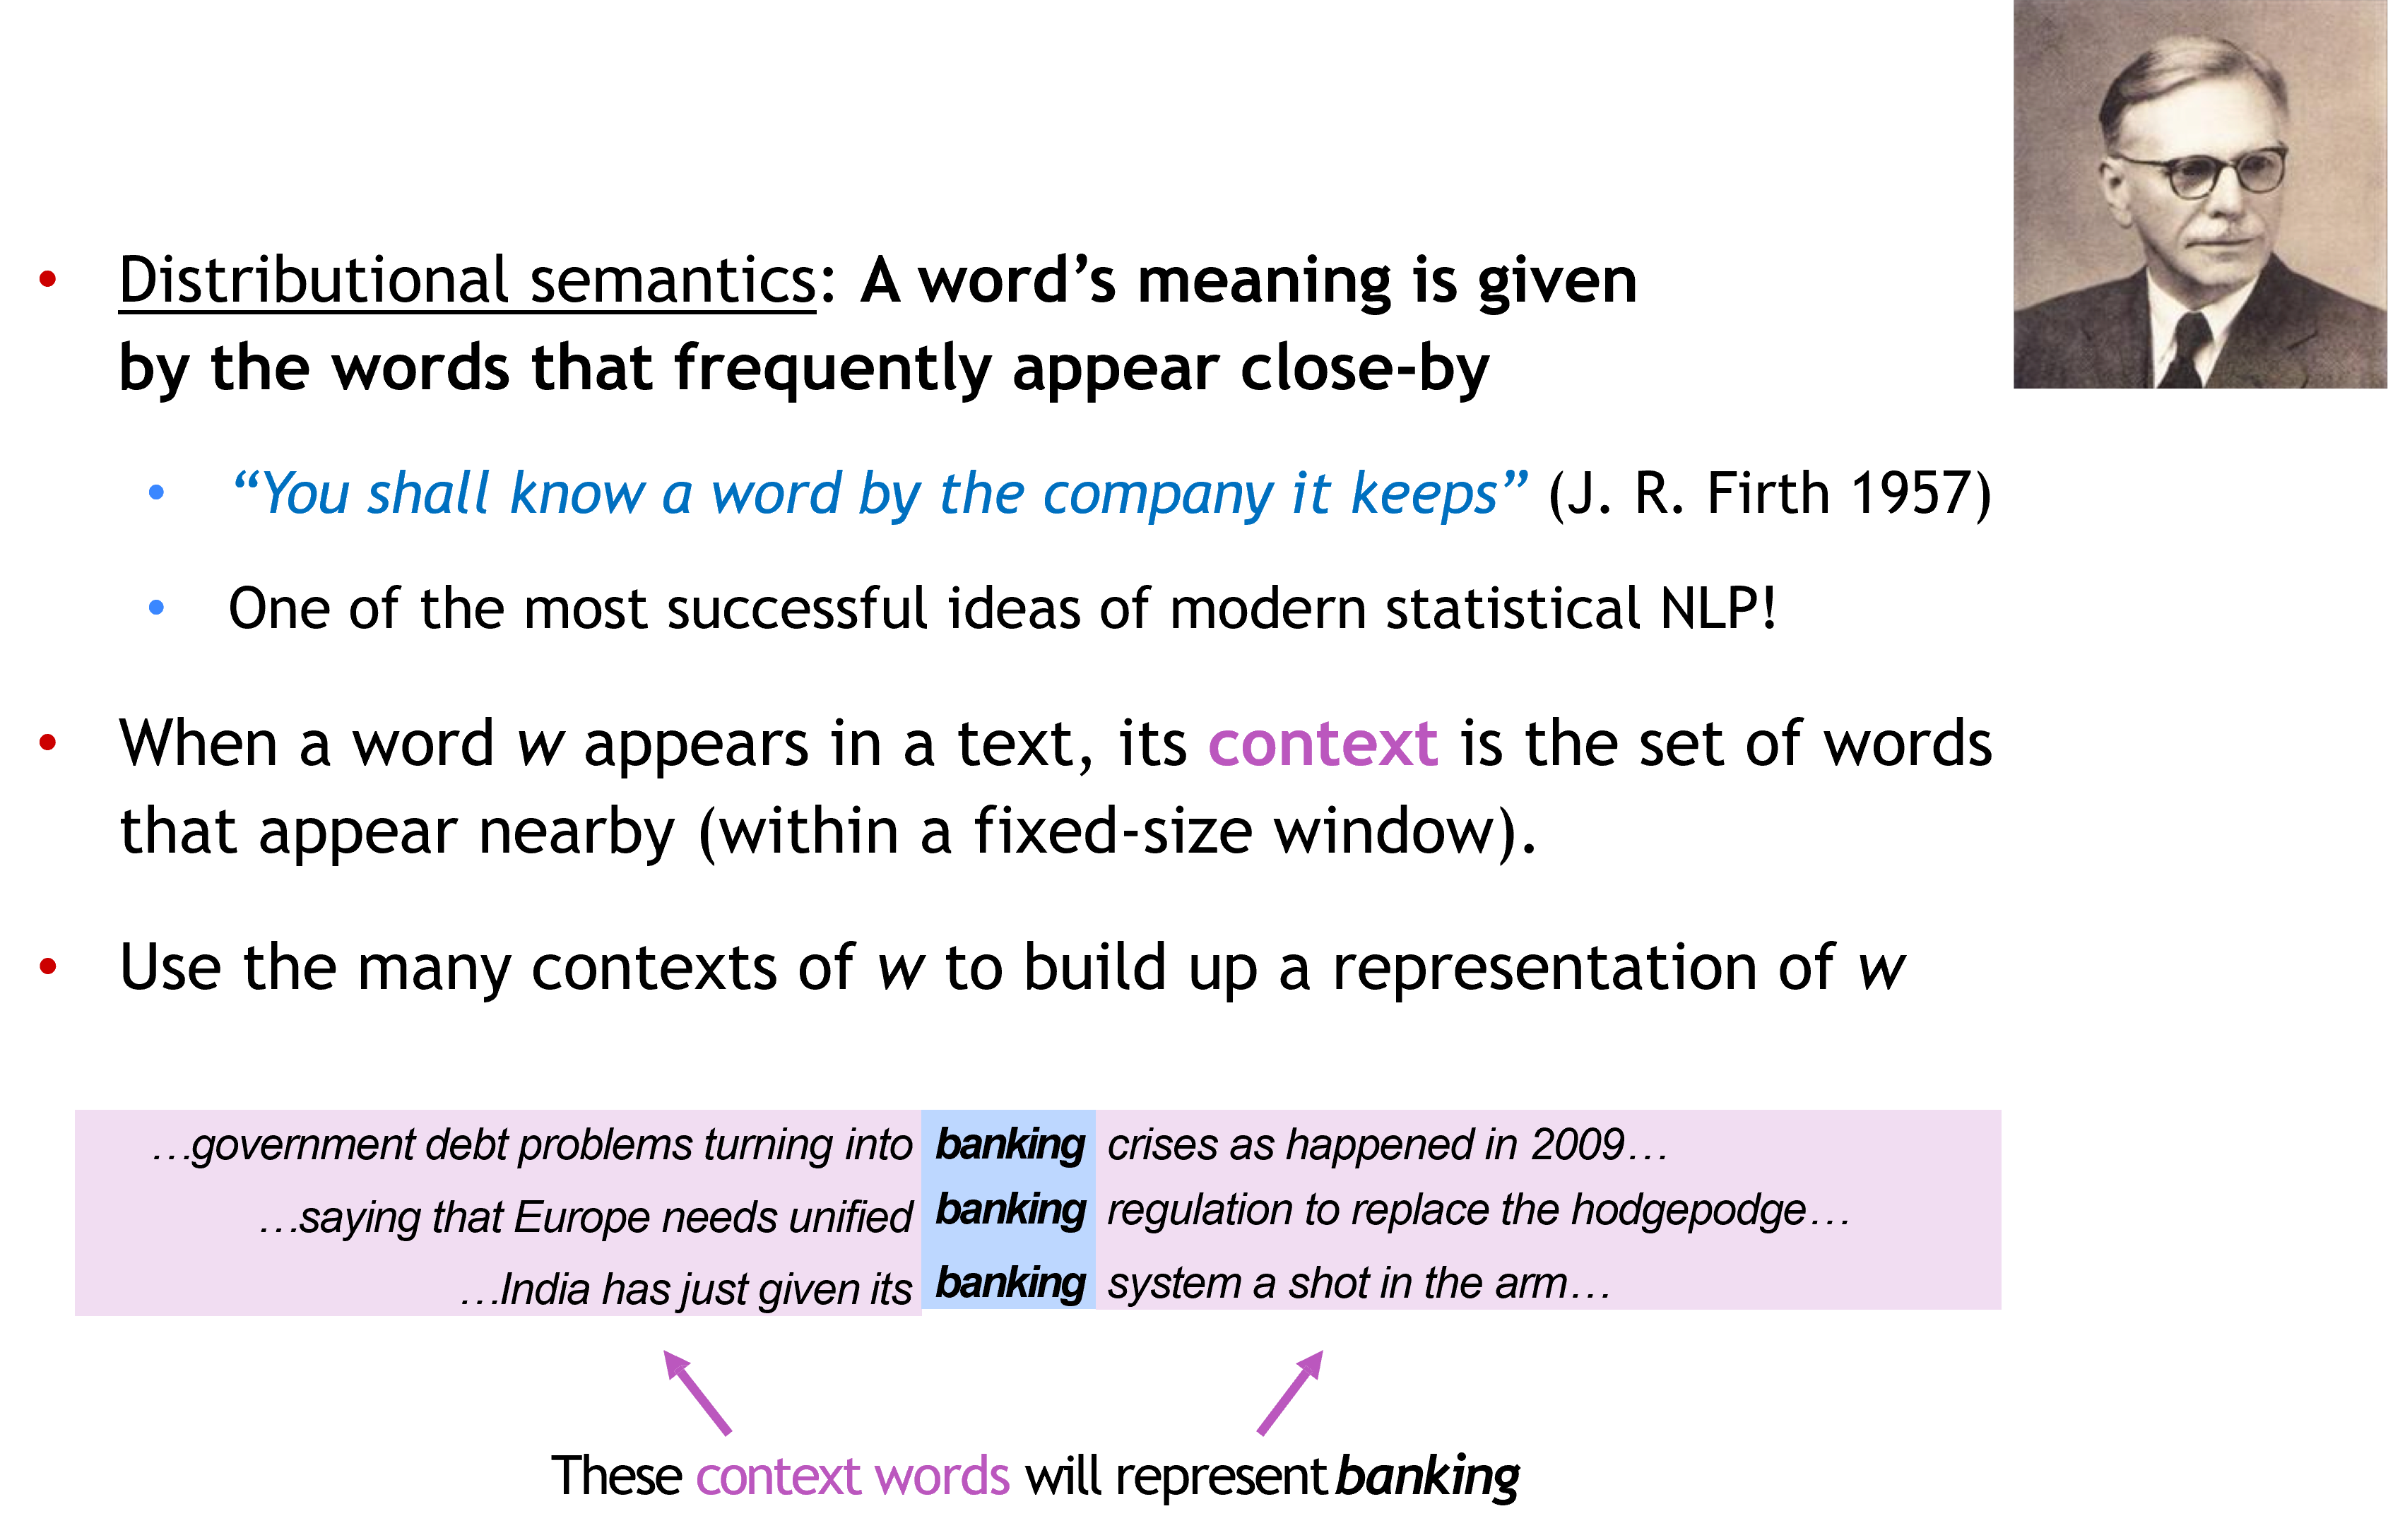
\includegraphics[width=\linewidth,keepaspectratio]{bert6}
\end{center}		  


{\tiny (Ref: CS224n: Natural Language Processing with Deep Learning - Christopher Manning)}

\end{frame}

%%%%%%%%%%%%%%%%%%%%%%%%%%%%%%%%%%%%%%%%%%%%%%%%%%%%%%%%%%%
\begin{frame}[fragile]\frametitle{What can we learn from reconstructing input?}

\begin{center}
Stanford University is located in $---------$	, California.
\end{center}		  

{\tiny (Ref: Language \& Machine Learning - John Hewitt)}
\end{frame}

%%%%%%%%%%%%%%%%%%%%%%%%%%%%%%%%%%%%%%%%%%%%%%%%%%%%%%%%%%%
\begin{frame}[fragile]\frametitle{What can we learn from reconstructing input?}

\begin{center}
I put $----------$ fork down on the table.
\end{center}		  

{\tiny (Ref: Language \& Machine Learning - John Hewitt)}
\end{frame}

%%%%%%%%%%%%%%%%%%%%%%%%%%%%%%%%%%%%%%%%%%%%%%%%%%%%%%%%%%%
\begin{frame}[fragile]\frametitle{What can we learn from reconstructing input?}

\begin{center}
The woman walked across the street, \\ checking for traffic over $----------$ shoulder.
\end{center}		  

{\tiny (Ref: Language \& Machine Learning - John Hewitt)}
\end{frame}

%%%%%%%%%%%%%%%%%%%%%%%%%%%%%%%%%%%%%%%%%%%%%%%%%%%%%%%%%%%
\begin{frame}[fragile]\frametitle{What can we learn from reconstructing input?}

\begin{center}
I went to the ocean to see the fish, turtles, seals, and $----------$.
\end{center}		  

{\tiny (Ref: Language \& Machine Learning - John Hewitt)}
\end{frame}

%%%%%%%%%%%%%%%%%%%%%%%%%%%%%%%%%%%%%%%%%%%%%%%%%%%%%%%%%%%
\begin{frame}[fragile]\frametitle{What can we learn from reconstructing input?}

\begin{center}
Overall, the value I got from the two hours watching \\ it was the sum total of the popcorn and the drink.\\
The movie was  $----------$.
\end{center}		  

{\tiny (Ref: Language \& Machine Learning - John Hewitt)}
\end{frame}

%%%%%%%%%%%%%%%%%%%%%%%%%%%%%%%%%%%%%%%%%%%%%%%%%%%%%%%%%%%
\begin{frame}[fragile]\frametitle{What can we learn from reconstructing input?}

\begin{center}
Iroh went into the kitchen to make some tea.\\
Standing next to Iroh, Zuko pondered his destiny.\\
Zuko left the  $----------$.
\end{center}		  

{\tiny (Ref: Language \& Machine Learning - John Hewitt)}
\end{frame}

%%%%%%%%%%%%%%%%%%%%%%%%%%%%%%%%%%%%%%%%%%%%%%%%%%%%%%%%%%%
\begin{frame}[fragile]\frametitle{What can we learn from reconstructing input?}

\begin{center}
I was thinking about the sequence that goes  \\ 1, 1, 2, 3, 5, 8, 13, 21,   $----------$.
\end{center}		  

{\tiny (Ref: Language \& Machine Learning - John Hewitt)}
\end{frame}

%%%%%%%%%%%%%%%%%%%%%%%%%%%%%%%%%%%%%%%%%%%%%%%%%%%%%%%%%%%
\begin{frame}[fragile]\frametitle{Word vectors}

We will build a dense vector for each word, chosen so that it is  similar to vectors of words that appear in similar contexts
	  
\begin{center}
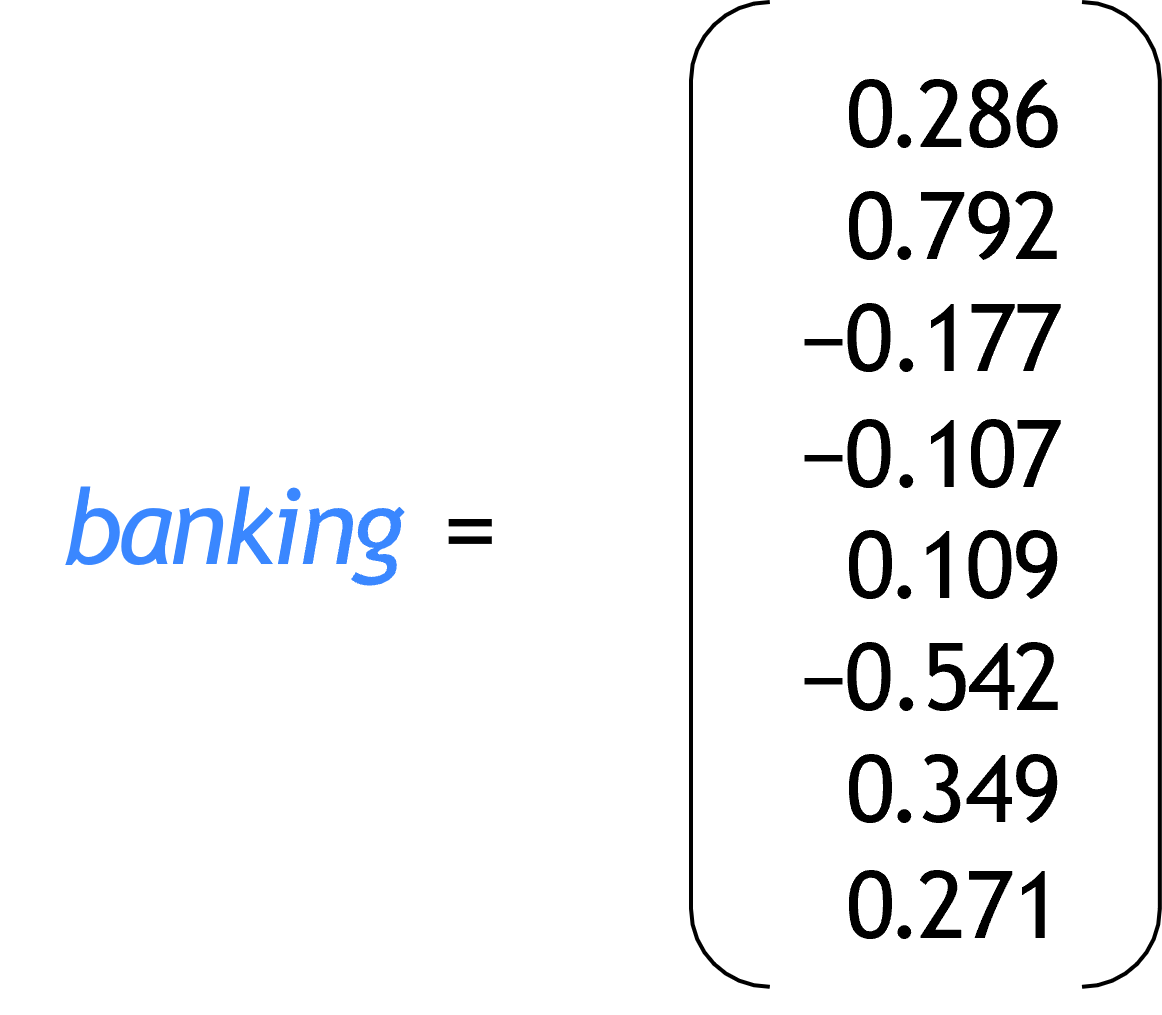
\includegraphics[width=0.5\linewidth,keepaspectratio]{bert7}
\end{center}		  
		
Note: word vectors are sometimes called word embeddings or  word representations. They are a distributed representation.

{\tiny (Ref: CS224n: Natural Language Processing with Deep Learning - Christopher Manning)}

\end{frame}

%%%%%%%%%%%%%%%%%%%%%%%%%%%%%%%%%%%%%%%%%%%%%%%%%%%%%%%%%%%
\begin{frame}[fragile]\frametitle{Word meaning as a neural word vector: visualization}

	  
\begin{center}
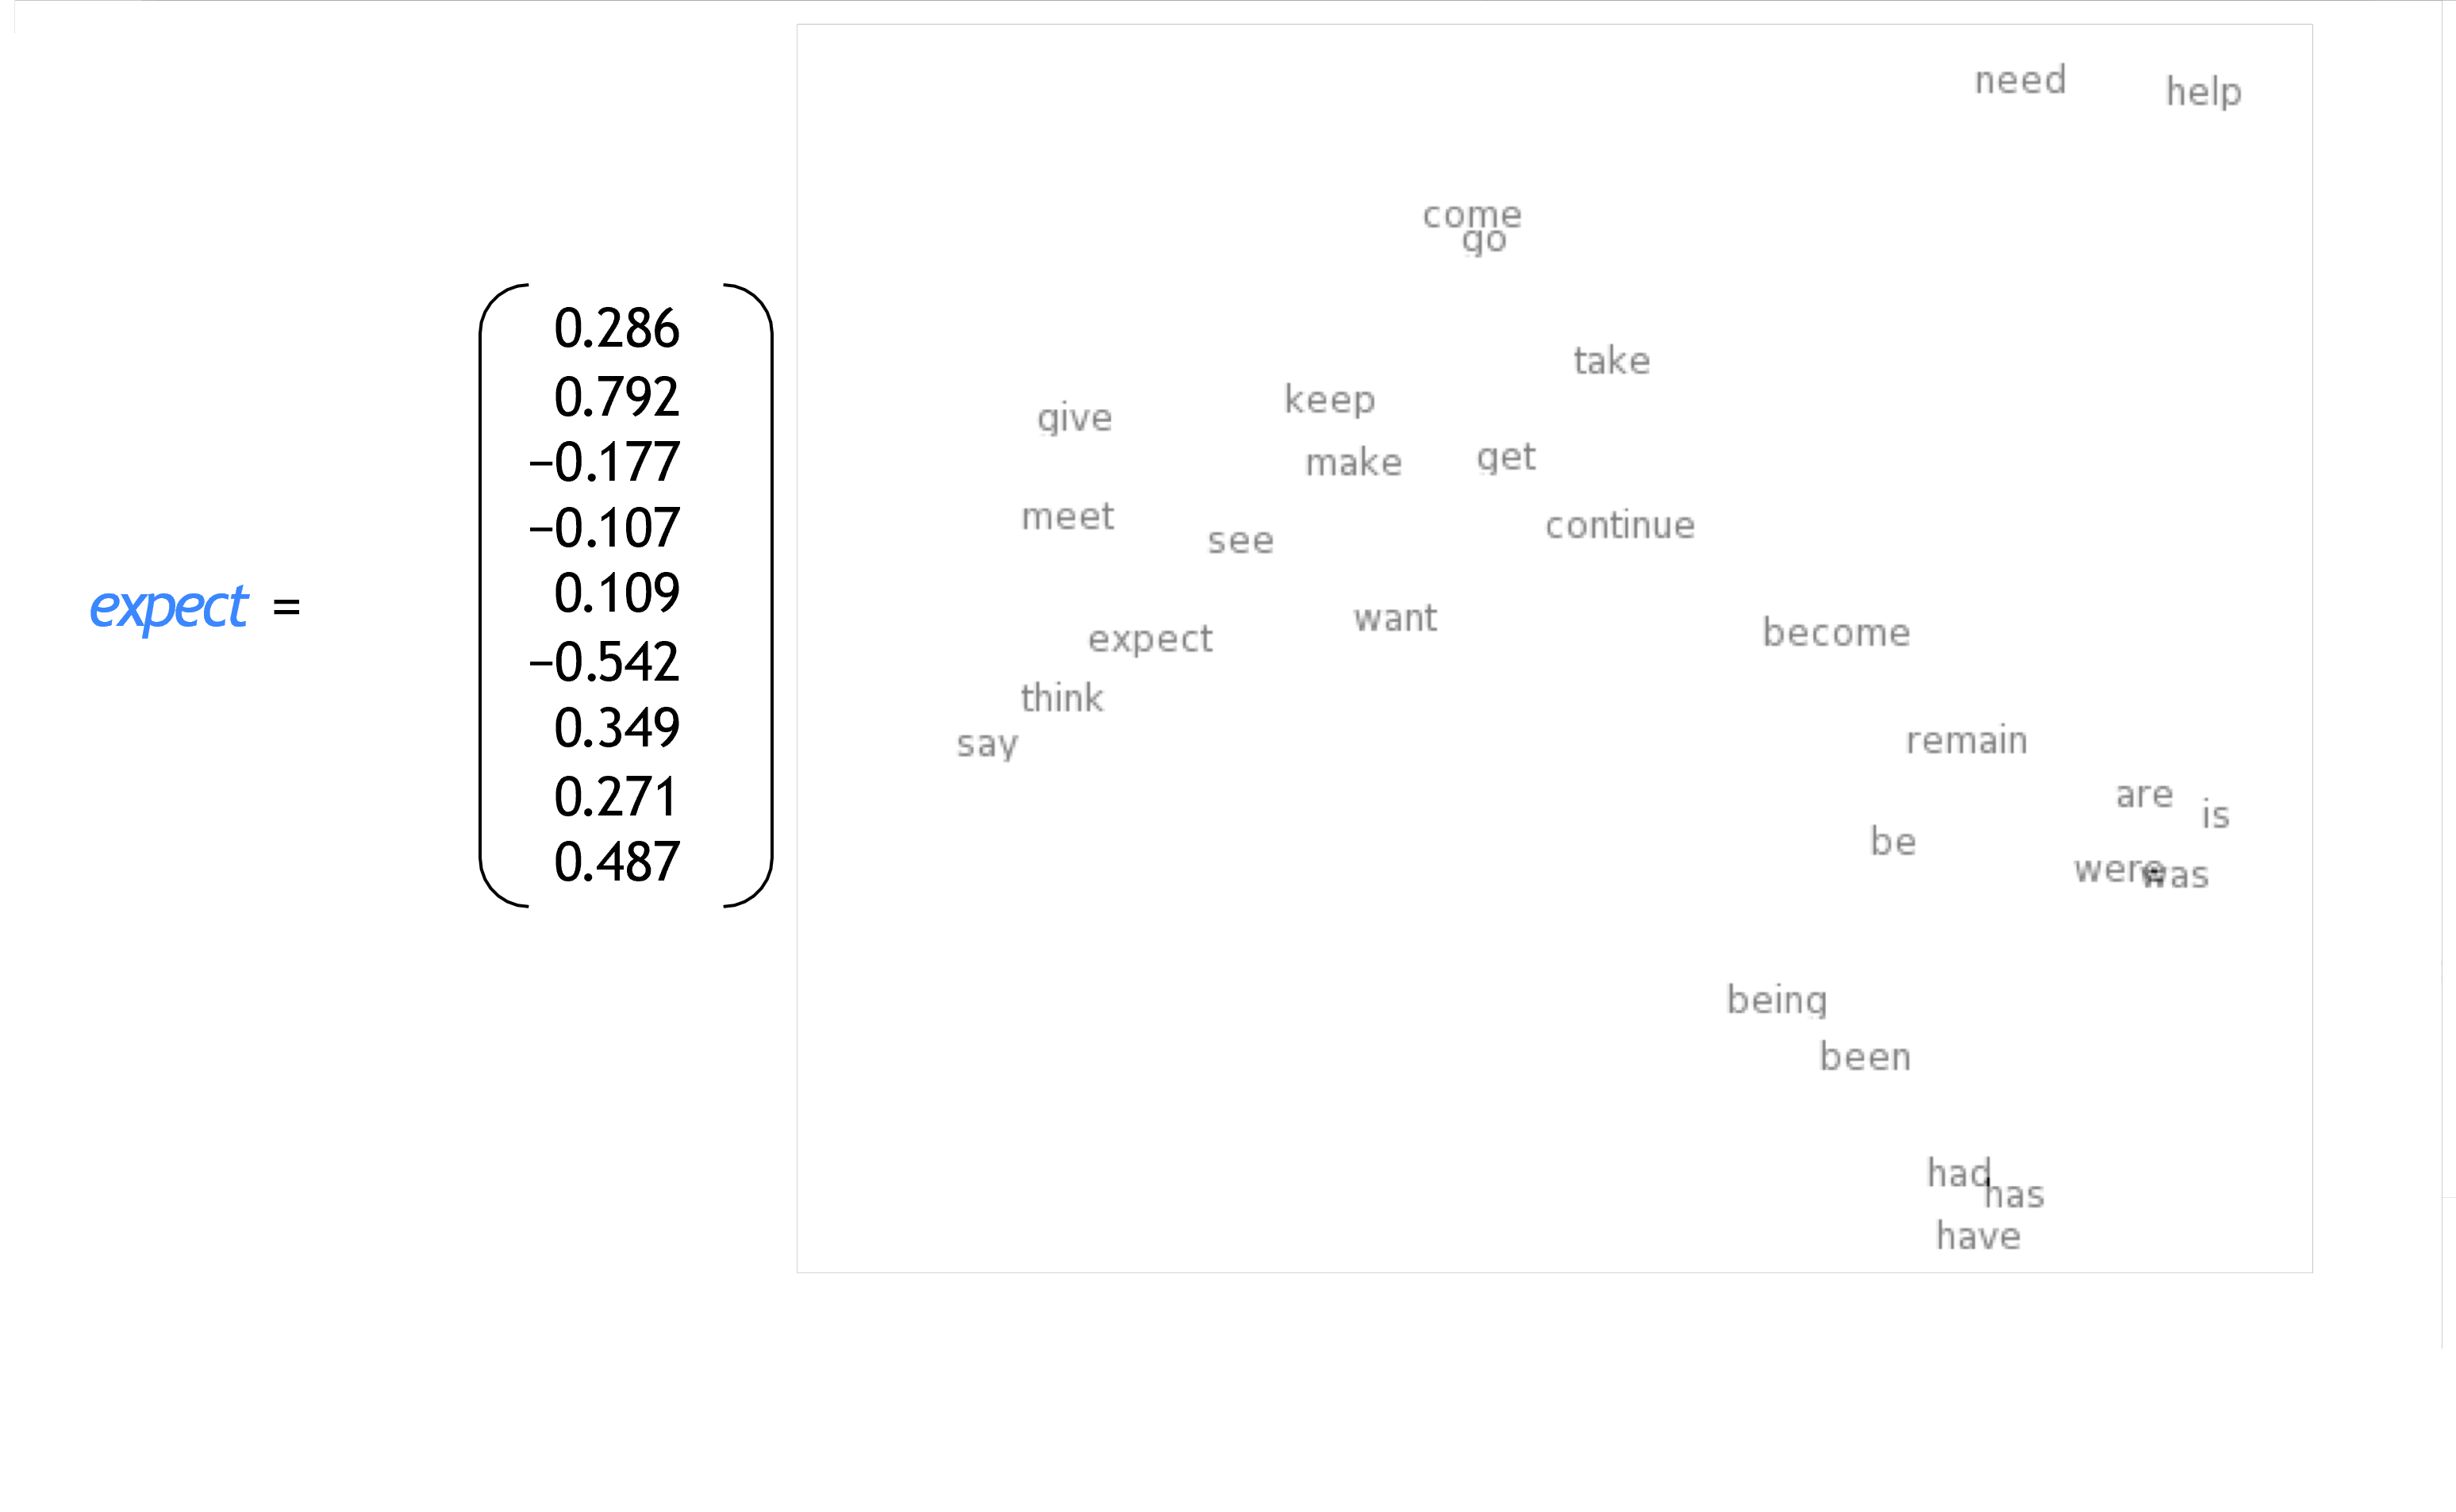
\includegraphics[width=\linewidth,keepaspectratio]{bert8}
\end{center}		  
		

{\tiny (Ref: CS224n: Natural Language Processing with Deep Learning - Christopher Manning)}

\end{frame}

%%%%%%%%%%%%%%%%%%%%%%%%%%%%%%%%%%%%%%%%%%%%%%%%%%%%%%%%%%%
\begin{frame}[fragile]\frametitle{Word2Vec Overview}
Word2vec (Mikolov et al. 2013) is a framework for learning  word vectors

Idea:
\begin{itemize}
\item We have a large corpus of text
\item Every word in a fixed vocabulary is represented by a vector
\item Go through each position t in the text, which has a center word
c and context (“outside”) words o
\item Use the similarity of the word vectors for c and o to calculate  the probability of o given c (or vice versa)
\item Keep adjusting the word vectors to maximize this probability

\end{itemize}

{\tiny (Ref: CS224n: Natural Language Processing with Deep Learning - Christopher Manning)}

\end{frame}

%%%%%%%%%%%%%%%%%%%%%%%%%%%%%%%%%%%%%%%%%%%%%%%%%%%%%%%%%%%
\begin{frame}[fragile]\frametitle{Word2Vec Overview}
Example windows and process for computing  $P(w_{t+j}|w_t)$


\begin{center}
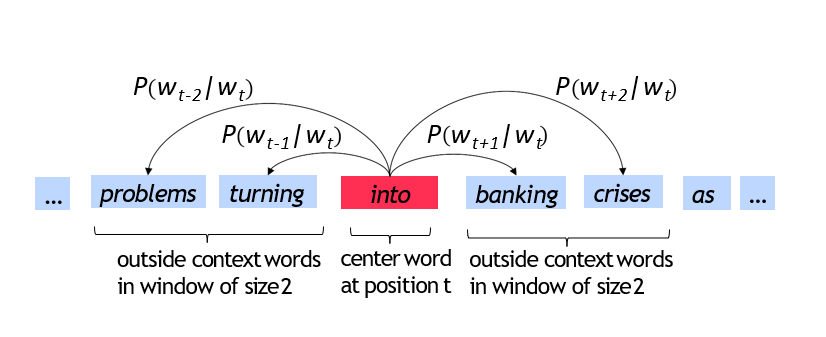
\includegraphics[width=\linewidth,keepaspectratio]{bert9}
\end{center}	

{\tiny (Ref: CS224n: Natural Language Processing with Deep Learning - Christopher Manning)}

\end{frame}

%%%%%%%%%%%%%%%%%%%%%%%%%%%%%%%%%%%%%%%%%%%%%%%%%%%%%%%%%%%
\begin{frame}[fragile]\frametitle{Word2Vec Overview}
Example windows and process for computing  $P(w_{t+j}|w_t)$


\begin{center}
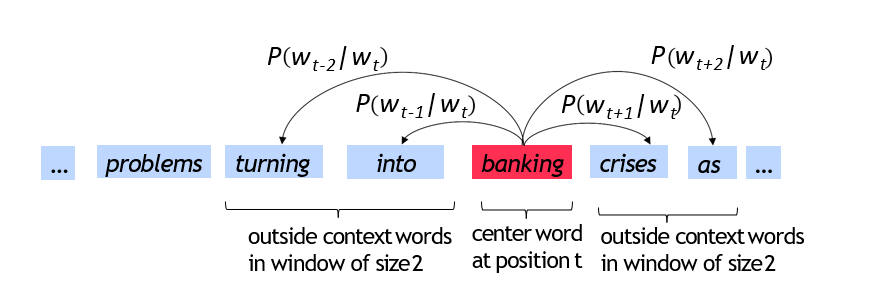
\includegraphics[width=\linewidth,keepaspectratio]{bert10}
\end{center}	

{\tiny (Ref: CS224n: Natural Language Processing with Deep Learning - Christopher Manning)}

\end{frame}

%%%%%%%%%%%%%%%%%%%%%%%%%%%%%%%%%%%%%%%%%%%%%%%%%%%%%%%%%%%
\begin{frame}[fragile]\frametitle{Word2Vec objective function}


\begin{center}
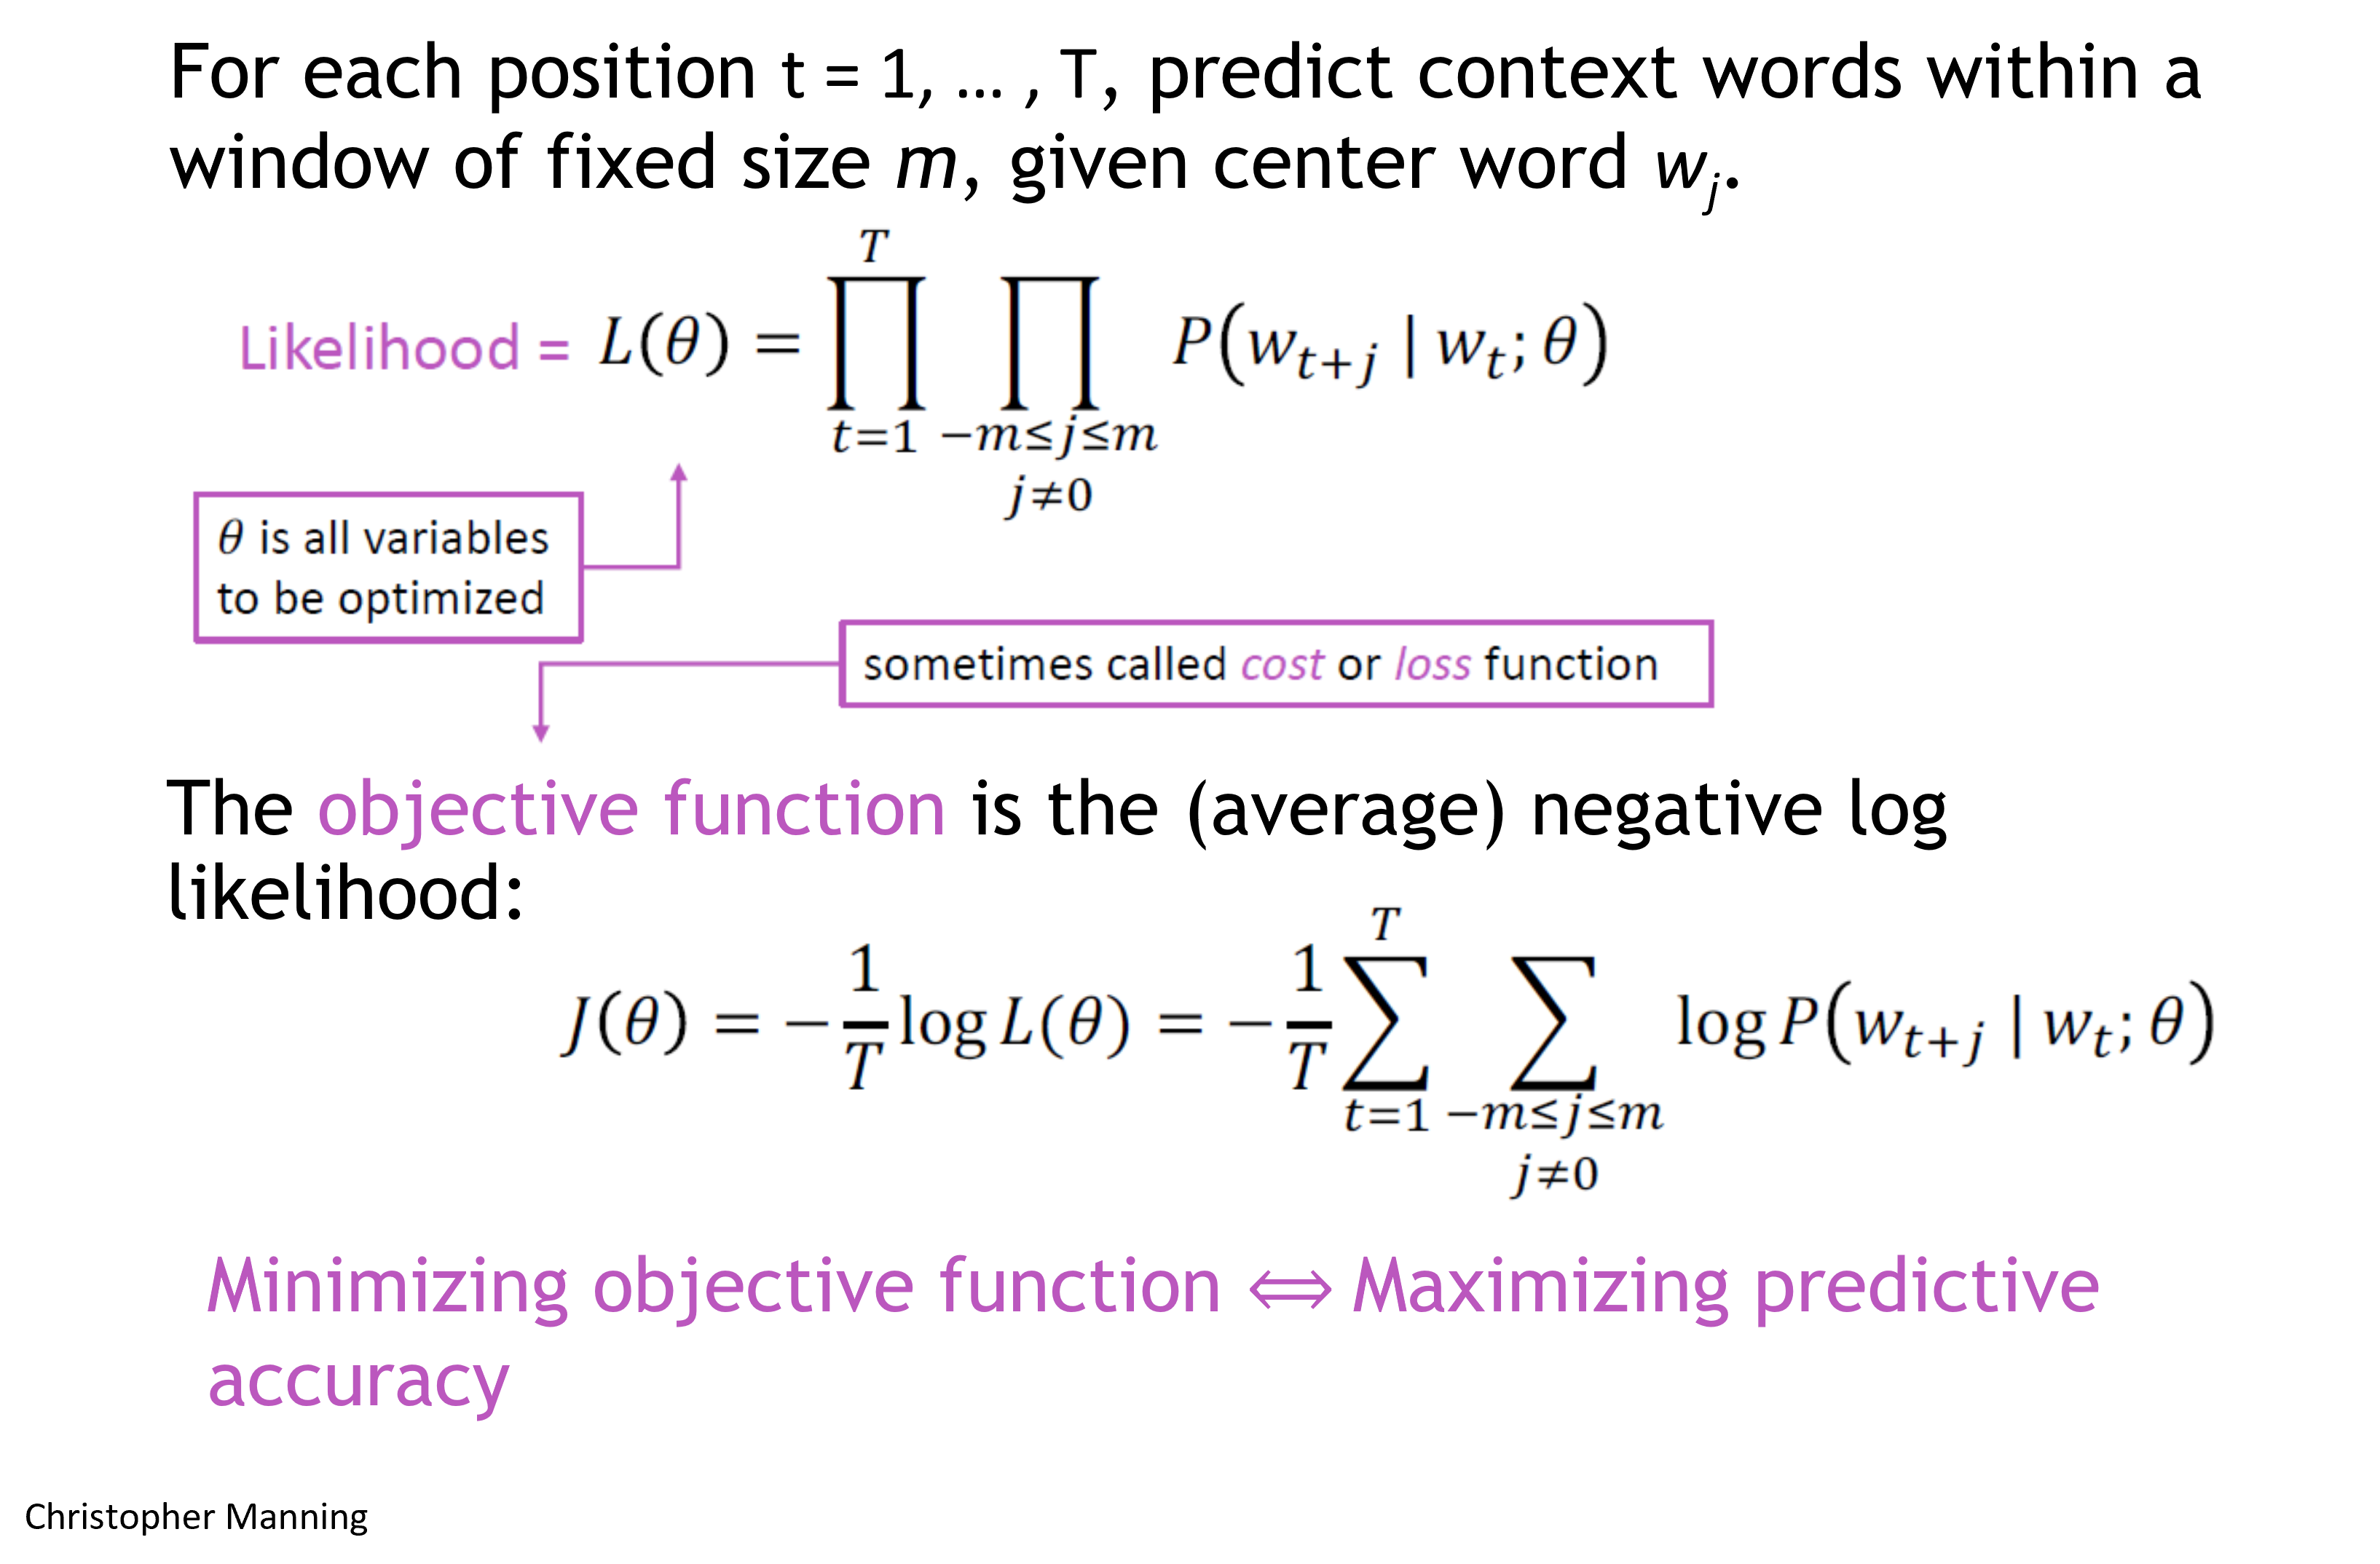
\includegraphics[width=0.9\linewidth,keepaspectratio]{bert11}
\end{center}	

{\tiny (Ref: CS224n: Natural Language Processing with Deep Learning - Christopher Manning)}

\end{frame}

%%%%%%%%%%%%%%%%%%%%%%%%%%%%%%%%%%%%%%%%%%%%%%%%%%%%%%%%%%%
\begin{frame}[fragile]\frametitle{Word2Vec objective function}


\begin{center}
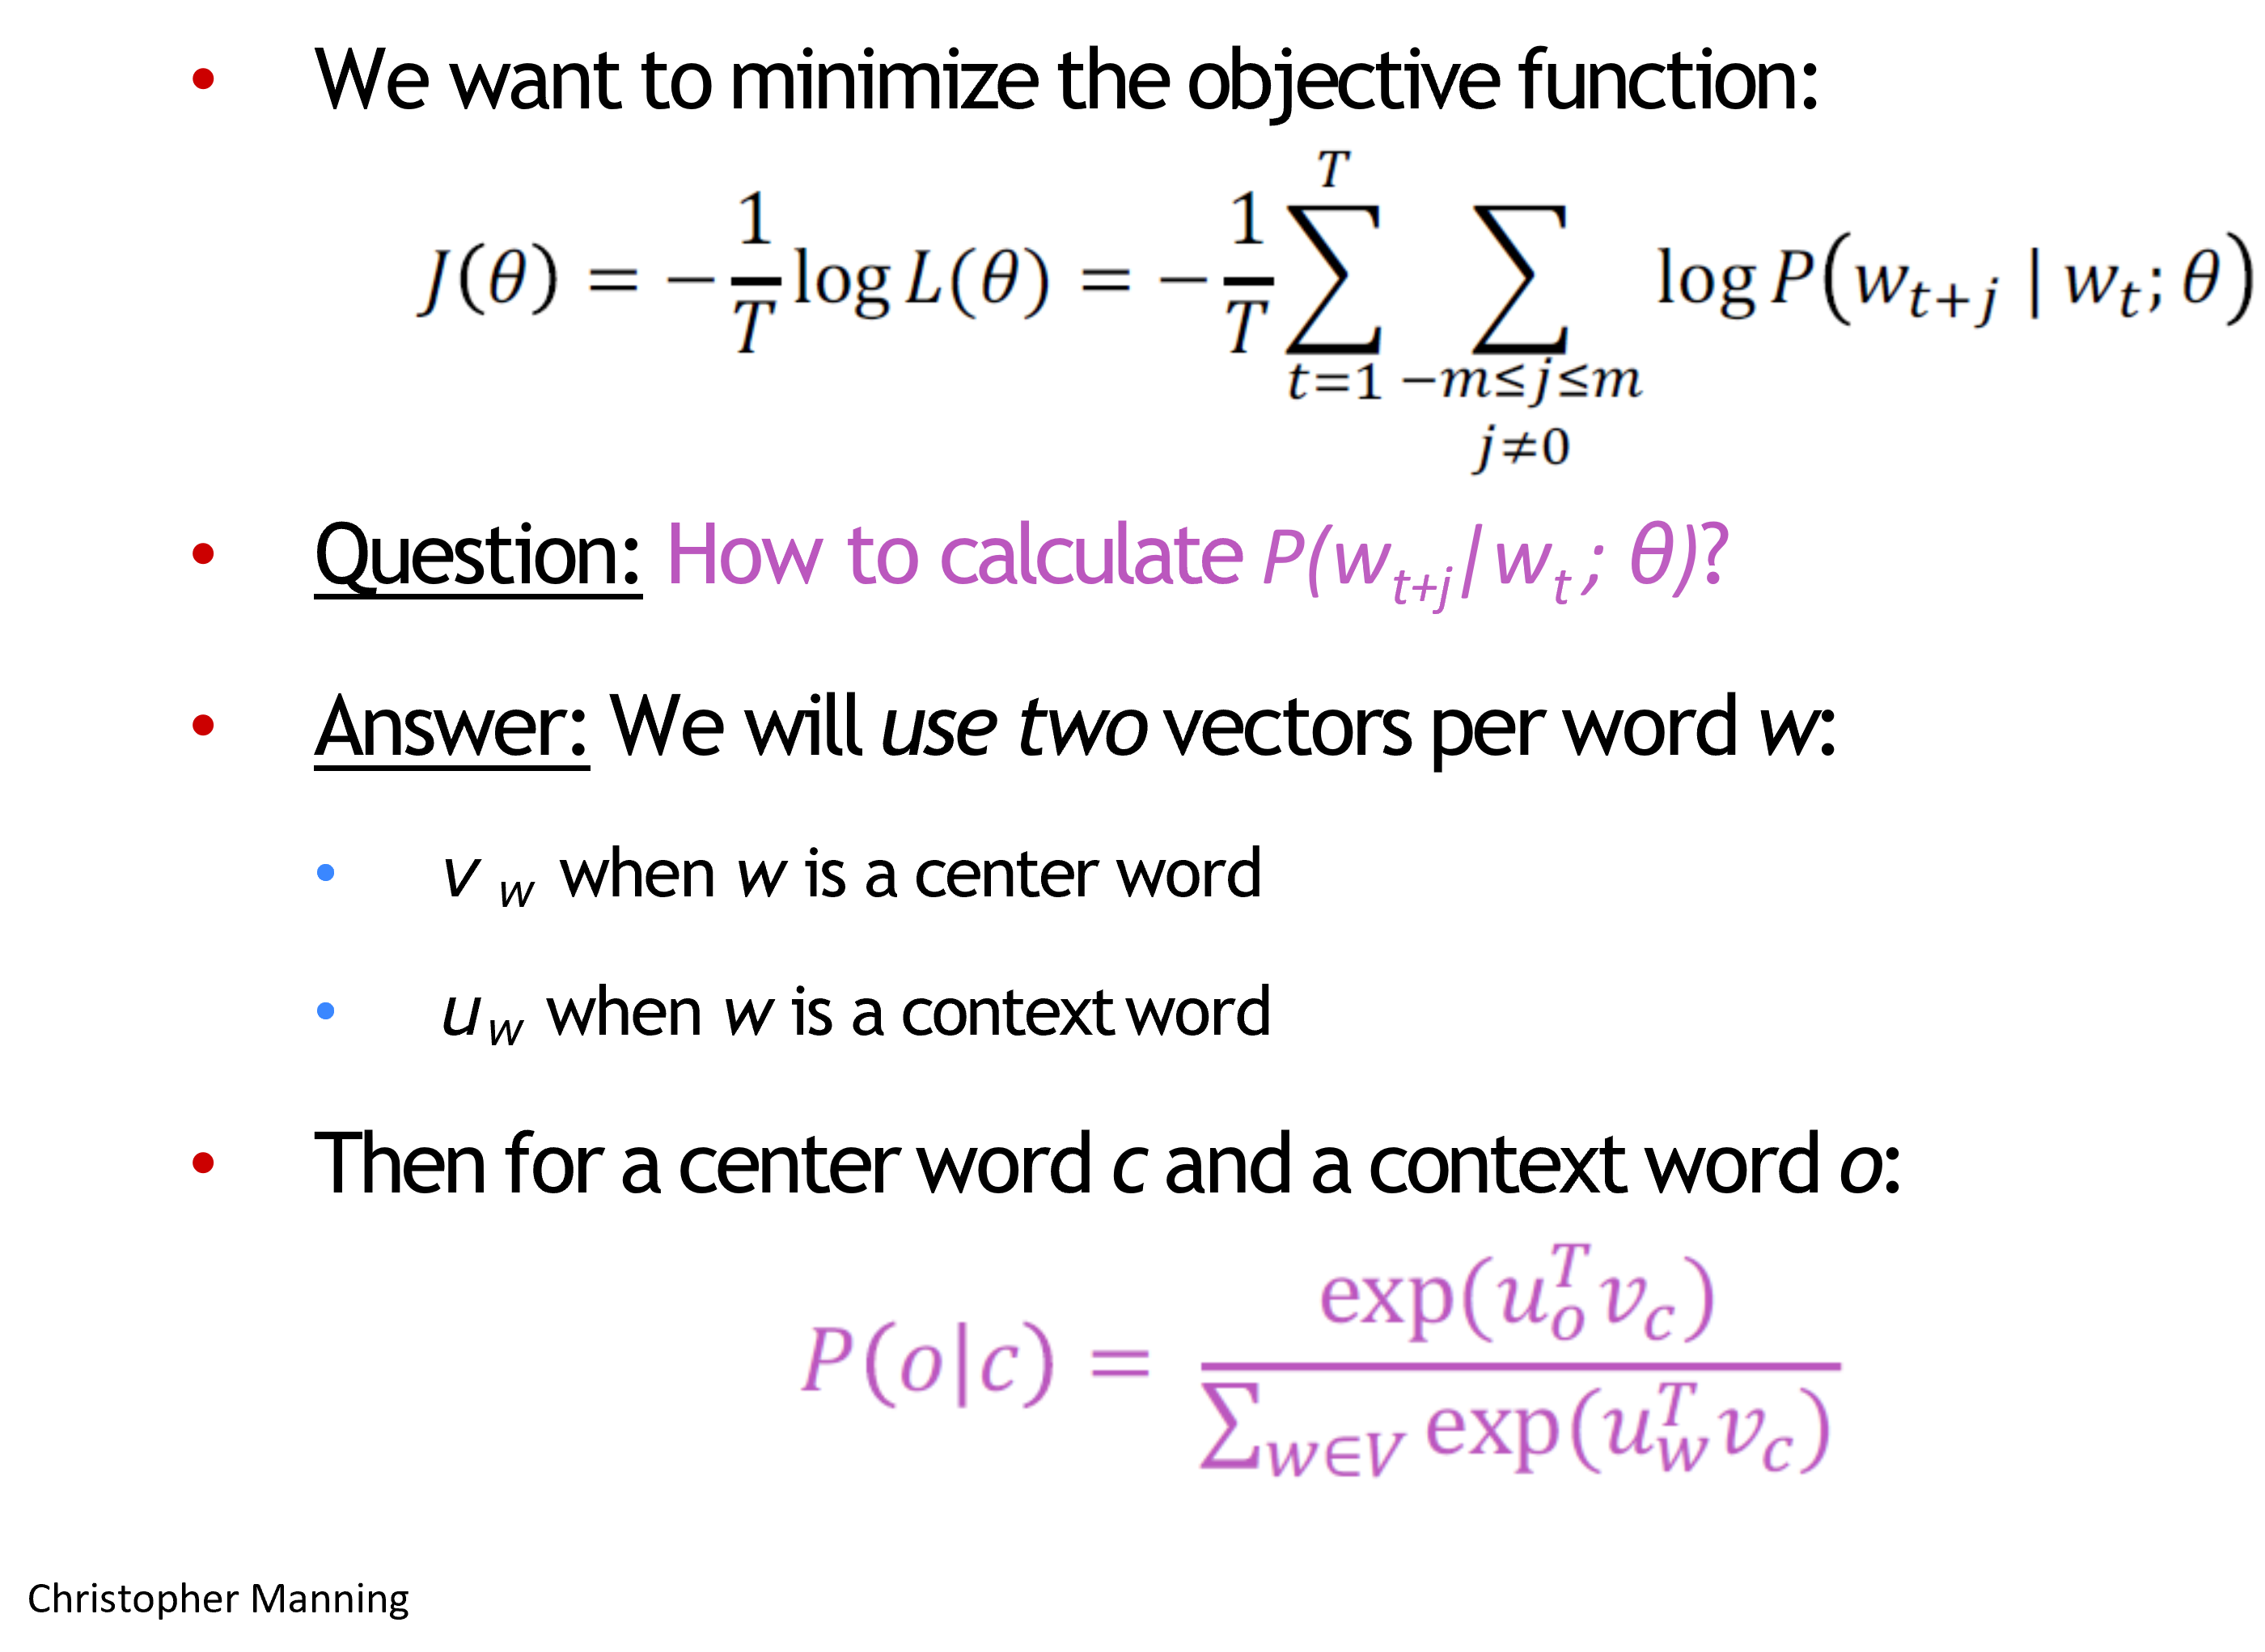
\includegraphics[width=0.9\linewidth,keepaspectratio]{bert12}
\end{center}	

{\tiny (Ref: CS224n: Natural Language Processing with Deep Learning - Christopher Manning)}

\end{frame}

%%%%%%%%%%%%%%%%%%%%%%%%%%%%%%%%%%%%%%%%%%%%%%%%%%%%%%%%%%%
\begin{frame}[fragile]\frametitle{Word2Vec prediction function}


\begin{center}
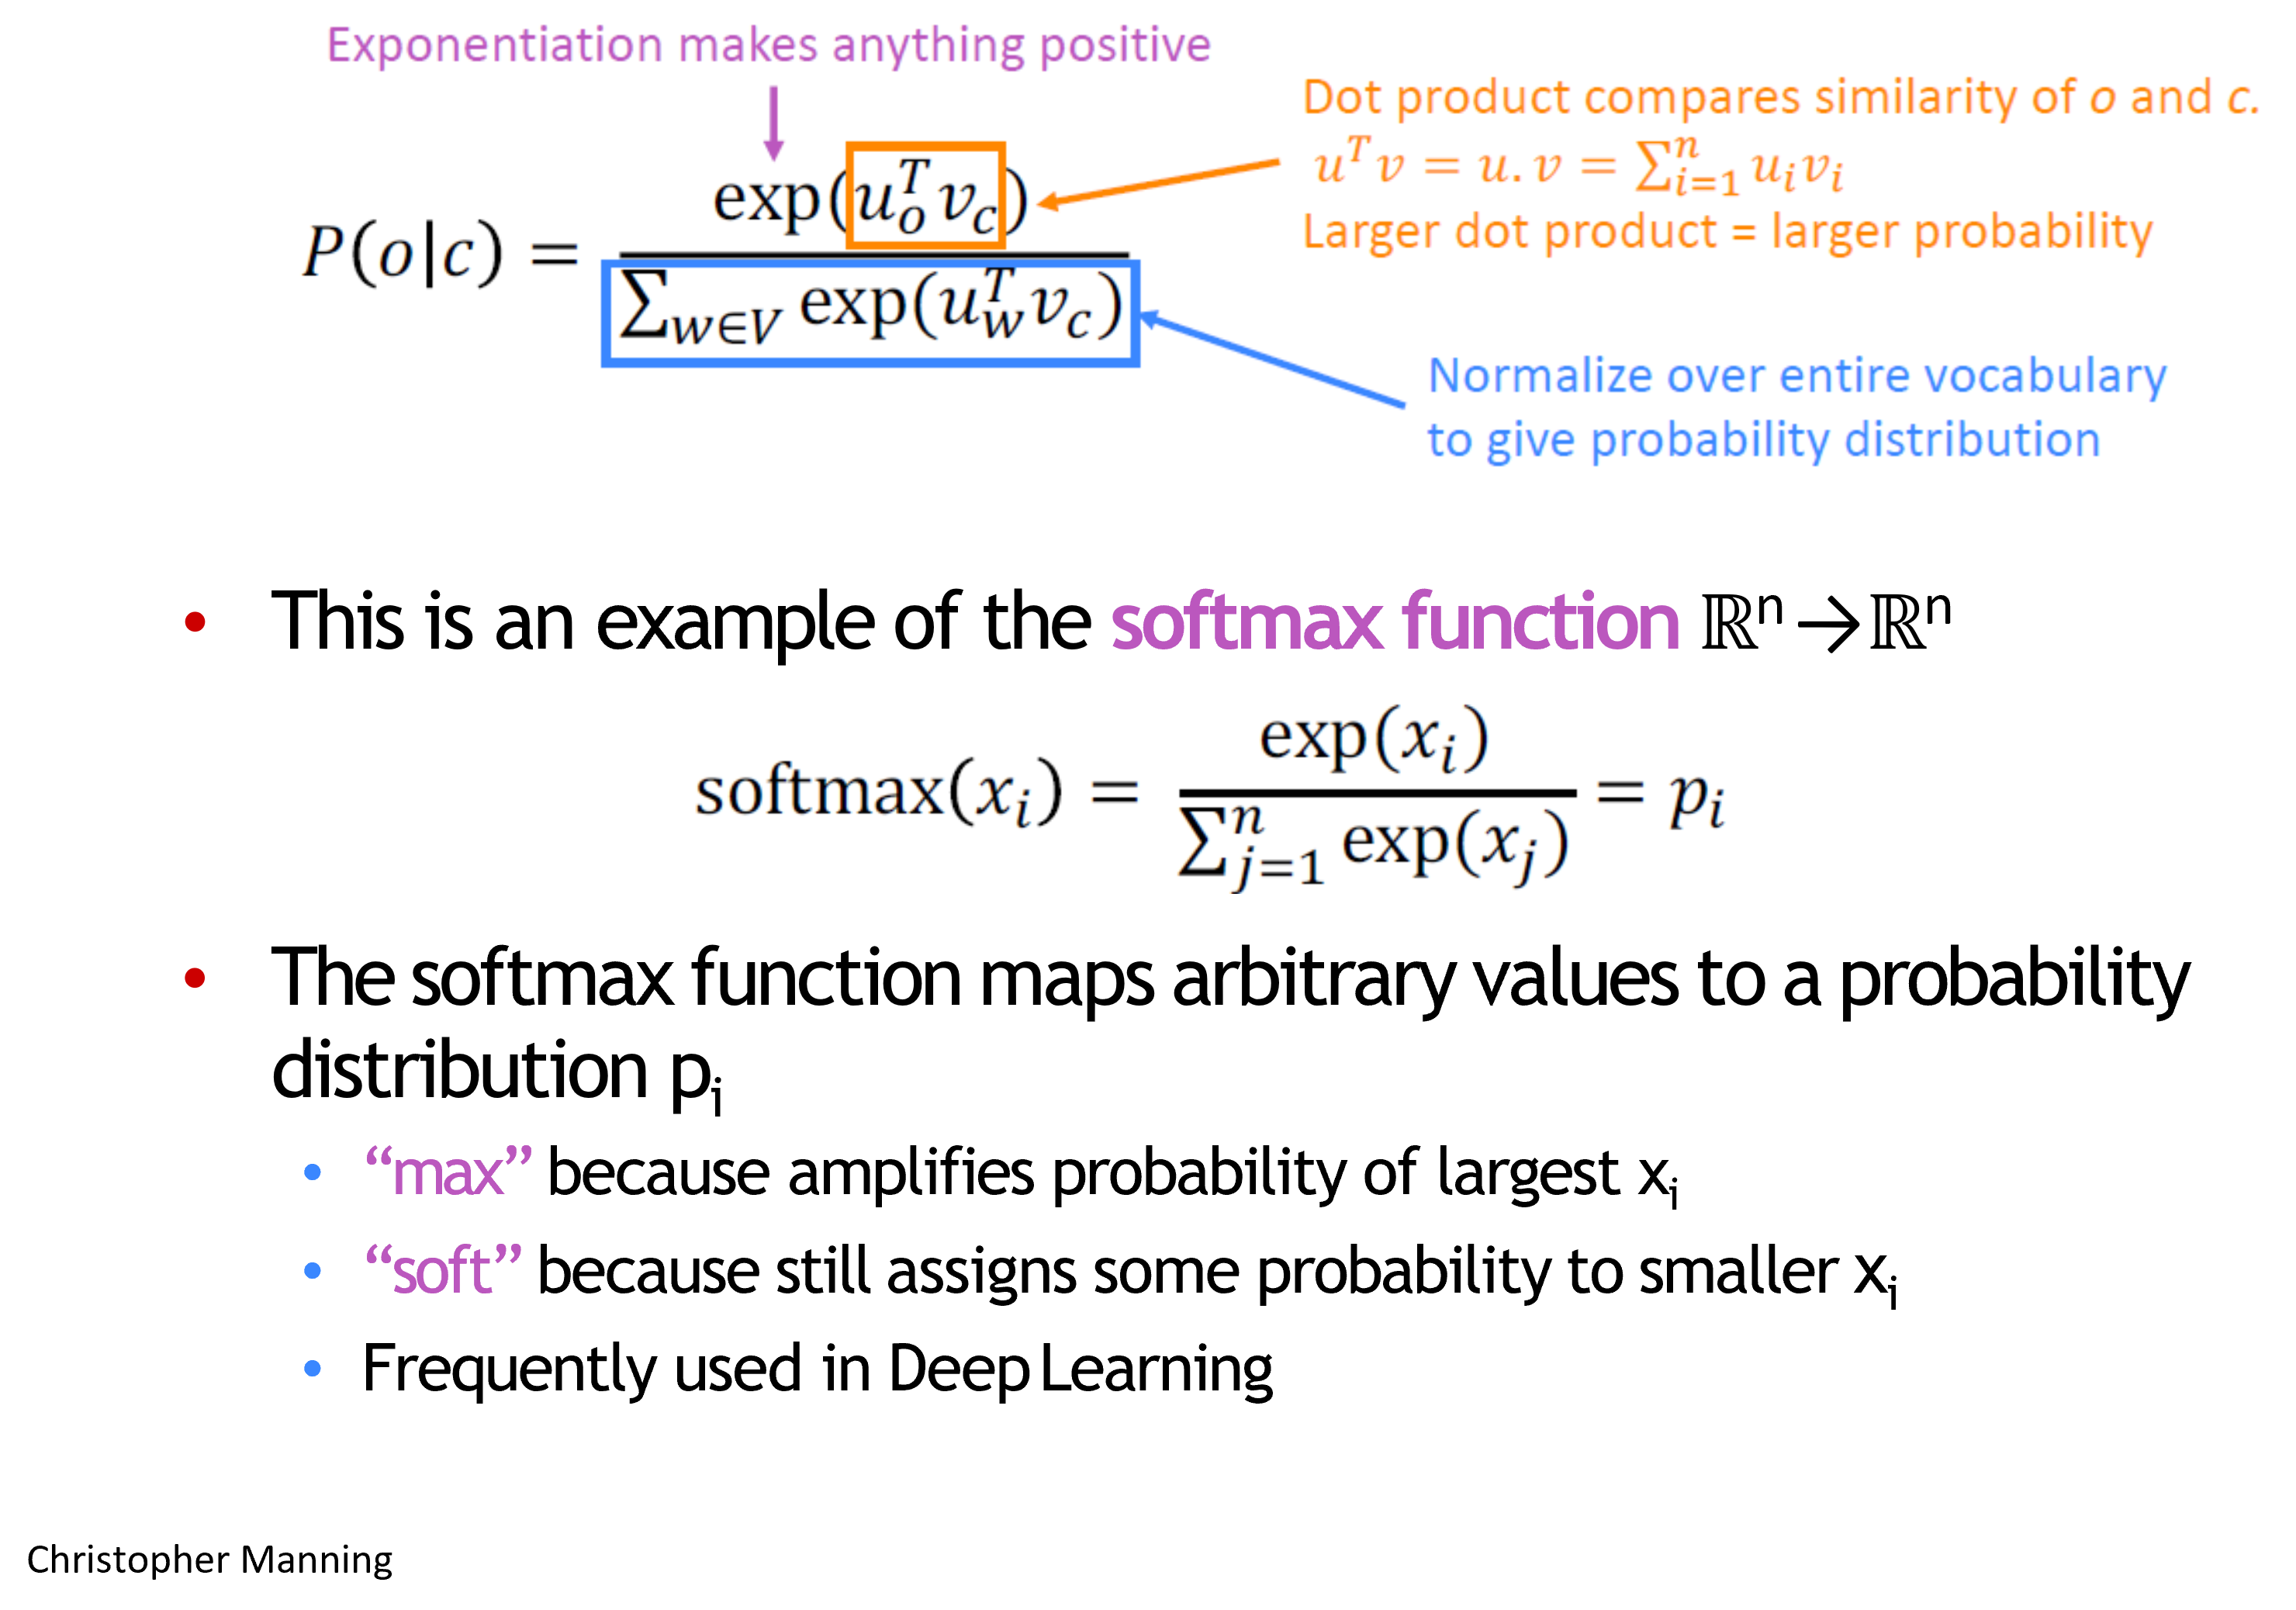
\includegraphics[width=0.9\linewidth,keepaspectratio]{bert13}
\end{center}	

{\tiny (Ref: CS224n: Natural Language Processing with Deep Learning - Christopher Manning)}

\end{frame}

%%%%%%%%%%%%%%%%%%%%%%%%%%%%%%%%%%%%%%%%%%%%%%%%%%%%%%%%%%%%%%%%%%%%%%%%%%%%%%%%%%
\begin{frame}[fragile]\frametitle{}
\begin{center}
{\Large Sequence Recurrence Models \\ \small RNNs and LSTMs}
\end{center}
\end{frame}


%%%%%%%%%%%%%%%%%%%%%%%%%%%%%%%%%%%%%%%%%%%%%%%%%%%%%%%%%%%
\begin{frame}[fragile]\frametitle{Sequence-to-Sequence (seq2seq)}

\begin{center}
See any issues with this traditional seq2seq paradigm?
\end{center}	

\end{frame}


%%%%%%%%%%%%%%%%%%%%%%%%%%%%%%%%%%%%%%%%%%%%%%%%%%%%%%%%%%%
\begin{frame}[fragile]\frametitle{Sequence-to-Sequence (seq2seq)}

\begin{center}
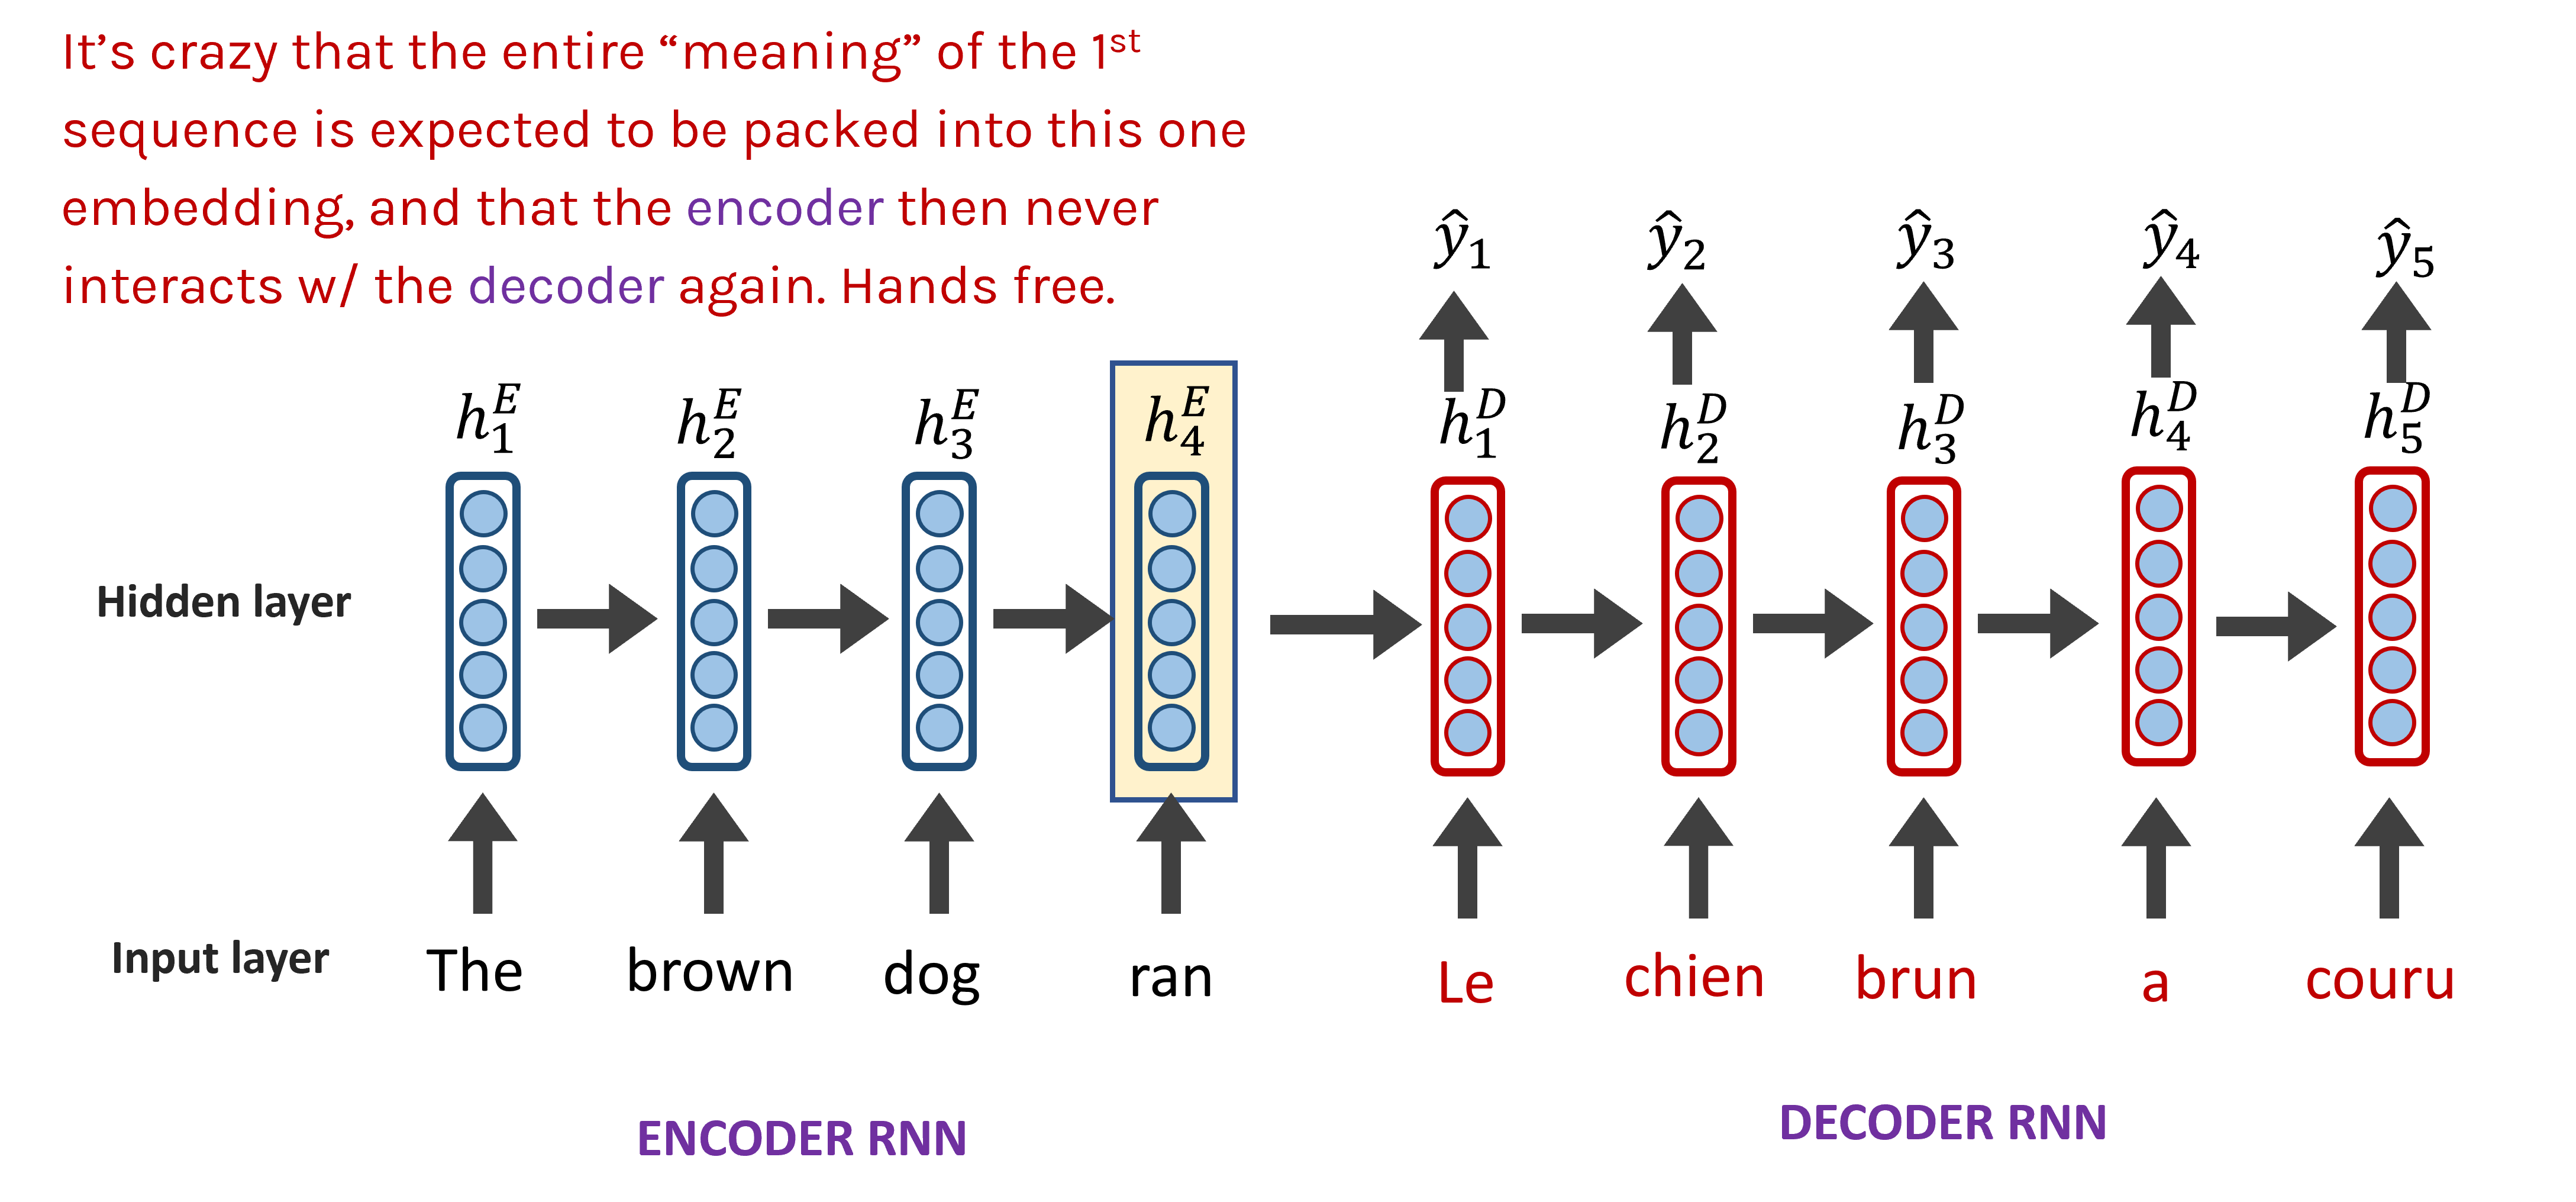
\includegraphics[width=\linewidth,keepaspectratio]{bert14}
\end{center}	

\end{frame}

%%%%%%%%%%%%%%%%%%%%%%%%%%%%%%%%%%%%%%%%%%%%%%%%%%%%%%%%%%%
\begin{frame}[fragile]\frametitle{Sequence-to-Sequence (seq2seq)}

\begin{center}
Instead, what if the decoder, at each step, pays {\bf attention} to a distribution of all of the encoder’s hidden states?
\end{center}	

\end{frame}

%%%%%%%%%%%%%%%%%%%%%%%%%%%%%%%%%%%%%%%%%%%%%%%%%%%%%%%%%%%
\begin{frame}[fragile]\frametitle{seq2seq + Attention}

Q: How do we determine how much to pay attention to each of the encoder’s hidden layers? 

\begin{center}
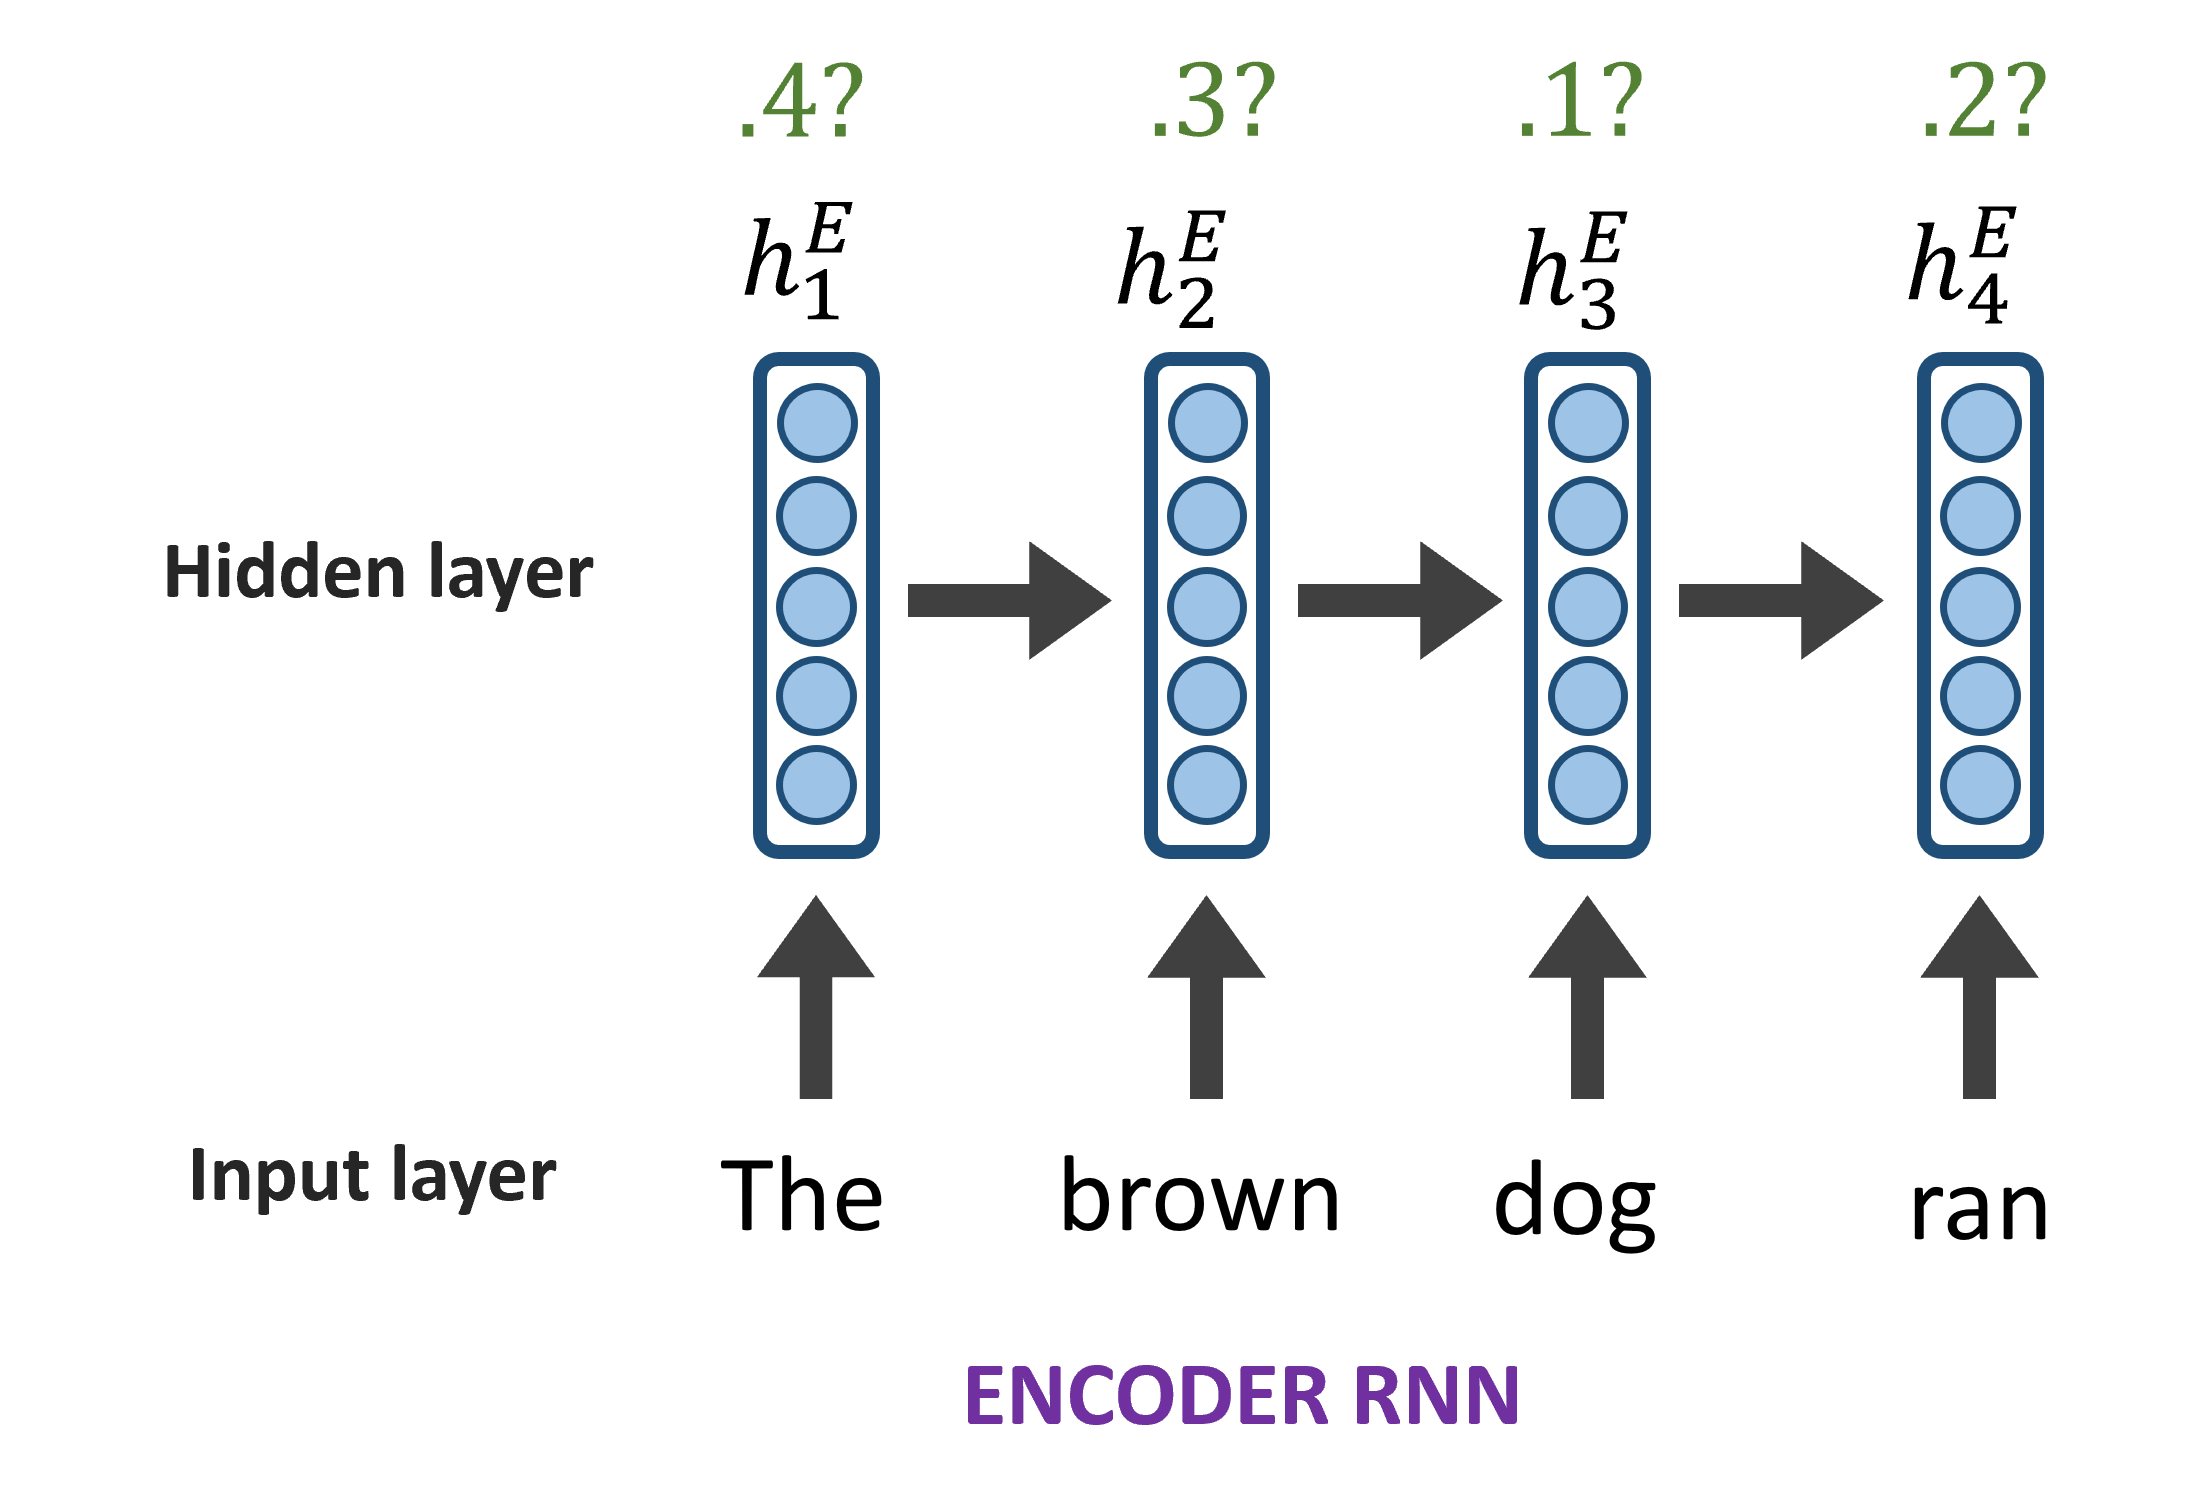
\includegraphics[width=0.8\linewidth,keepaspectratio]{bert15}
\end{center}	

\end{frame}


%%%%%%%%%%%%%%%%%%%%%%%%%%%%%%%%%%%%%%%%%%%%%%%%%%%%%%%%%%%
\begin{frame}[fragile]\frametitle{seq2seq + Attention}

Q: How do we determine how much to pay attention to each of the encoder’s hidden layers? 

A: Let’s base it on our decoder’s previous hidden state (our latest representation of meaning) and all of the encoder’s hidden layers!


\begin{center}
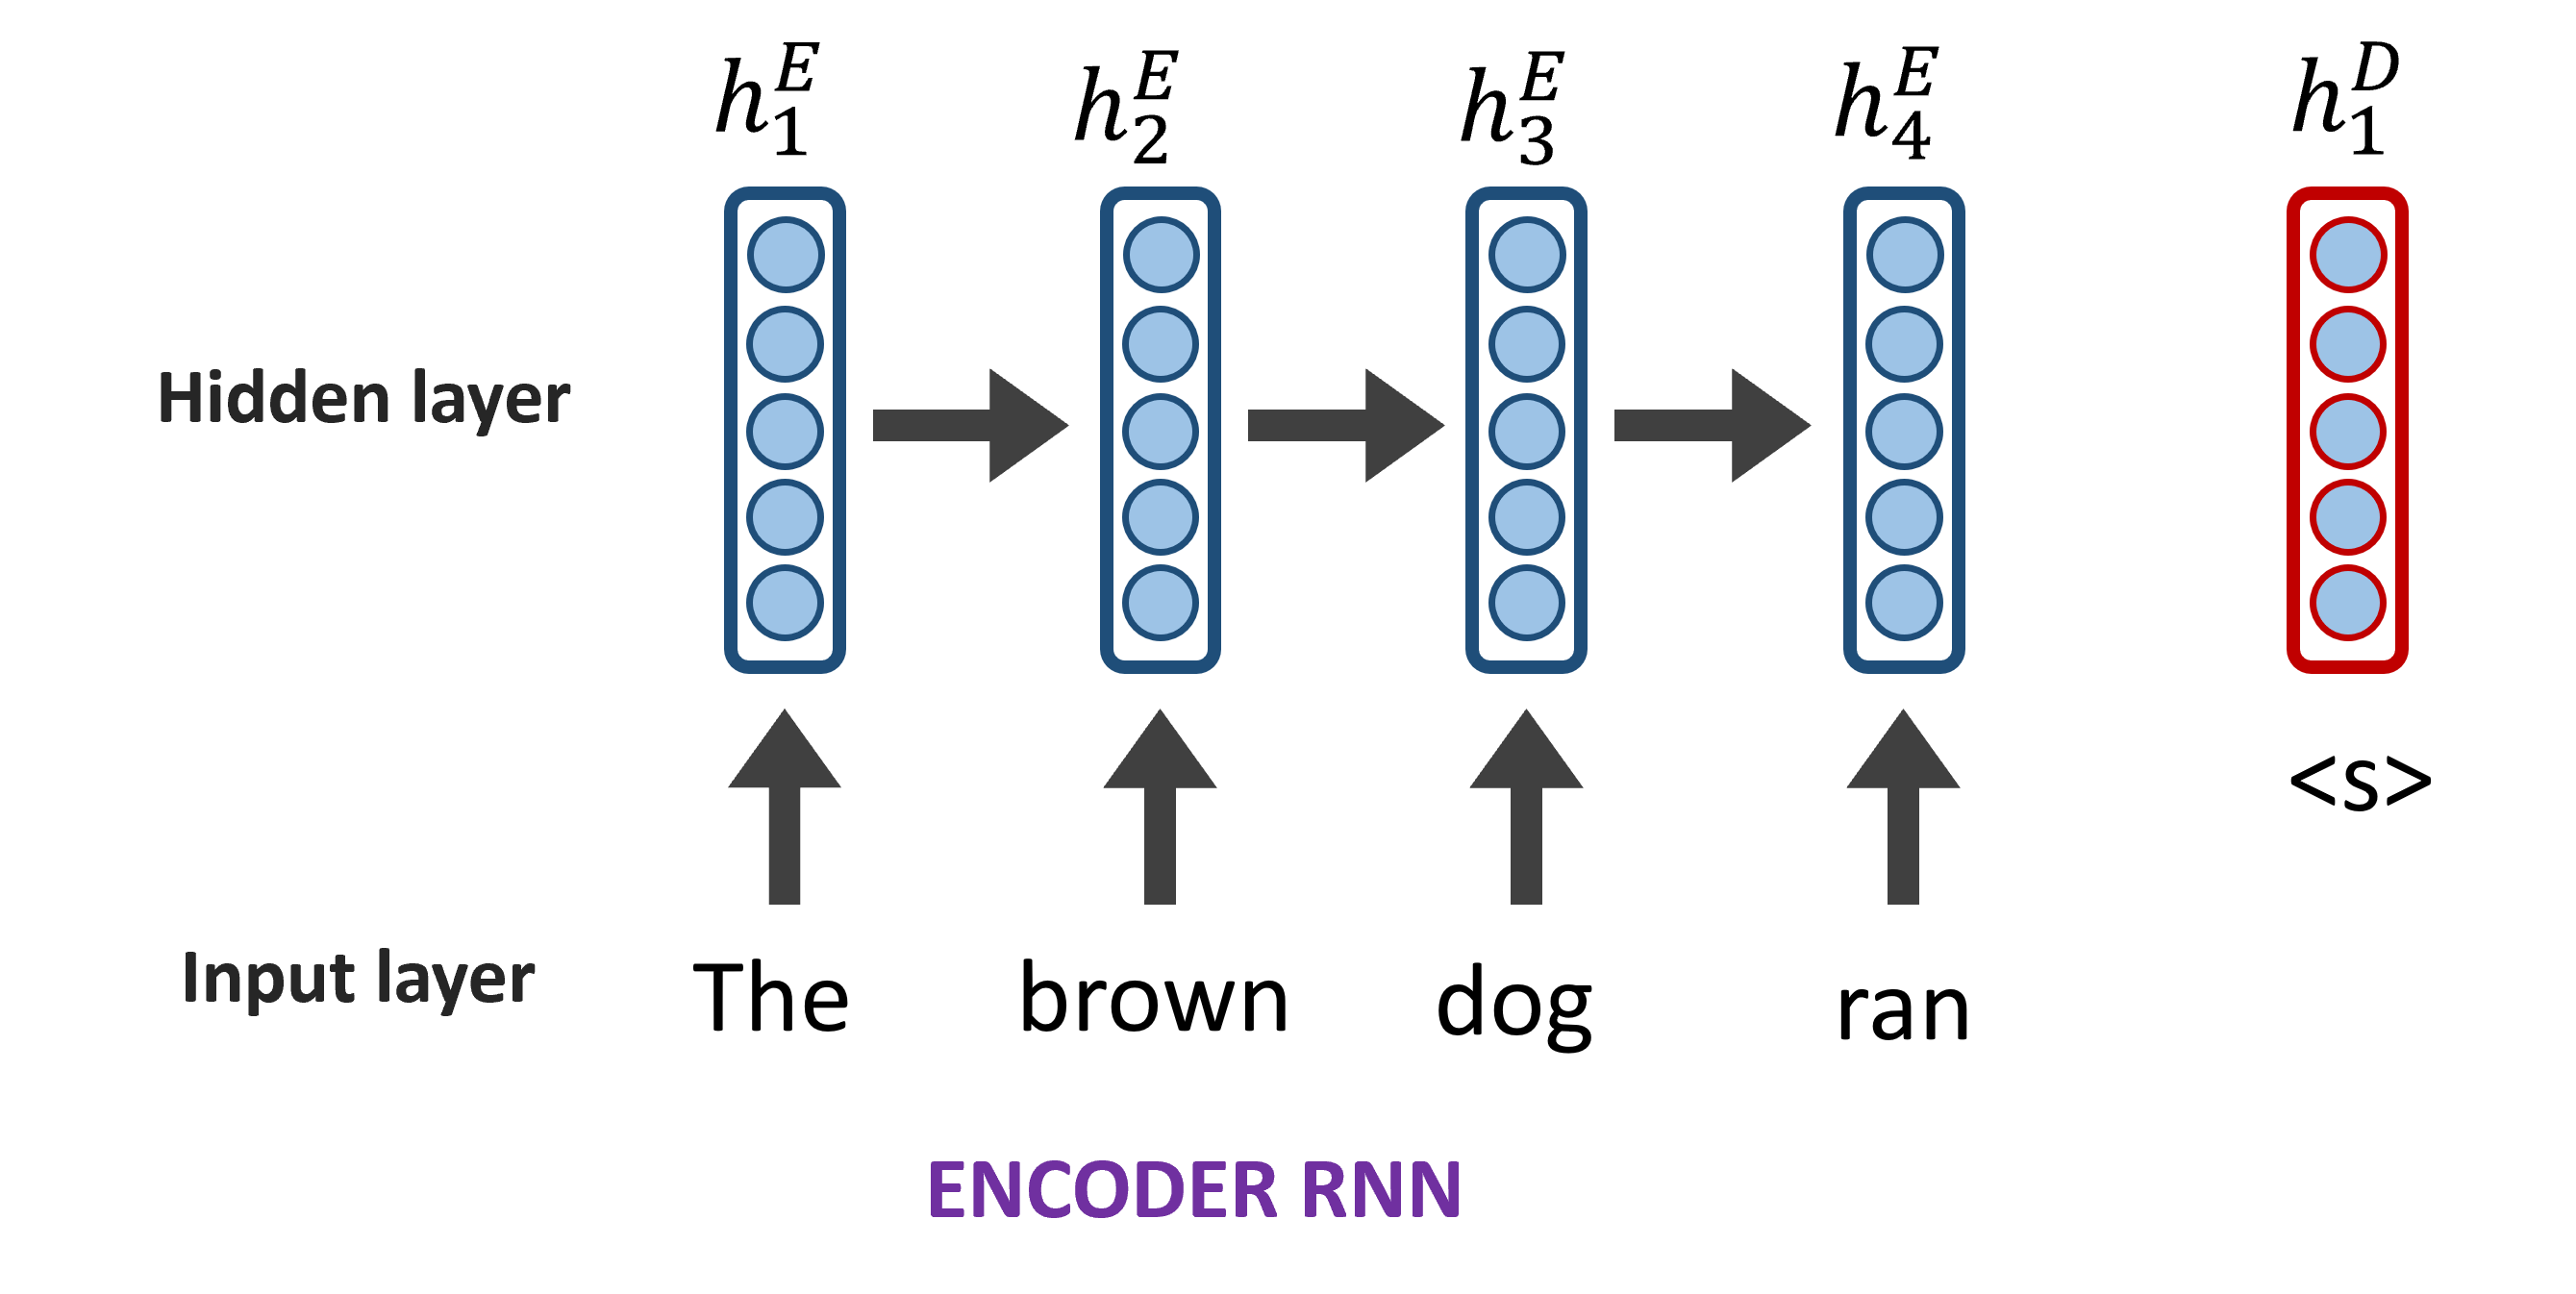
\includegraphics[width=0.8\linewidth,keepaspectratio]{bert16}
\end{center}	

\end{frame}

%%%%%%%%%%%%%%%%%%%%%%%%%%%%%%%%%%%%%%%%%%%%%%%%%%%%%%%%%%%
\begin{frame}[fragile]\frametitle{seq2seq + Attention}

Q: How do we determine how much to pay attention to each of the encoder’s hidden layers? 

A: Let’s base it on our decoder’s previous hidden state (our latest representation of meaning) and all of the encoder’s hidden layers!


\begin{center}
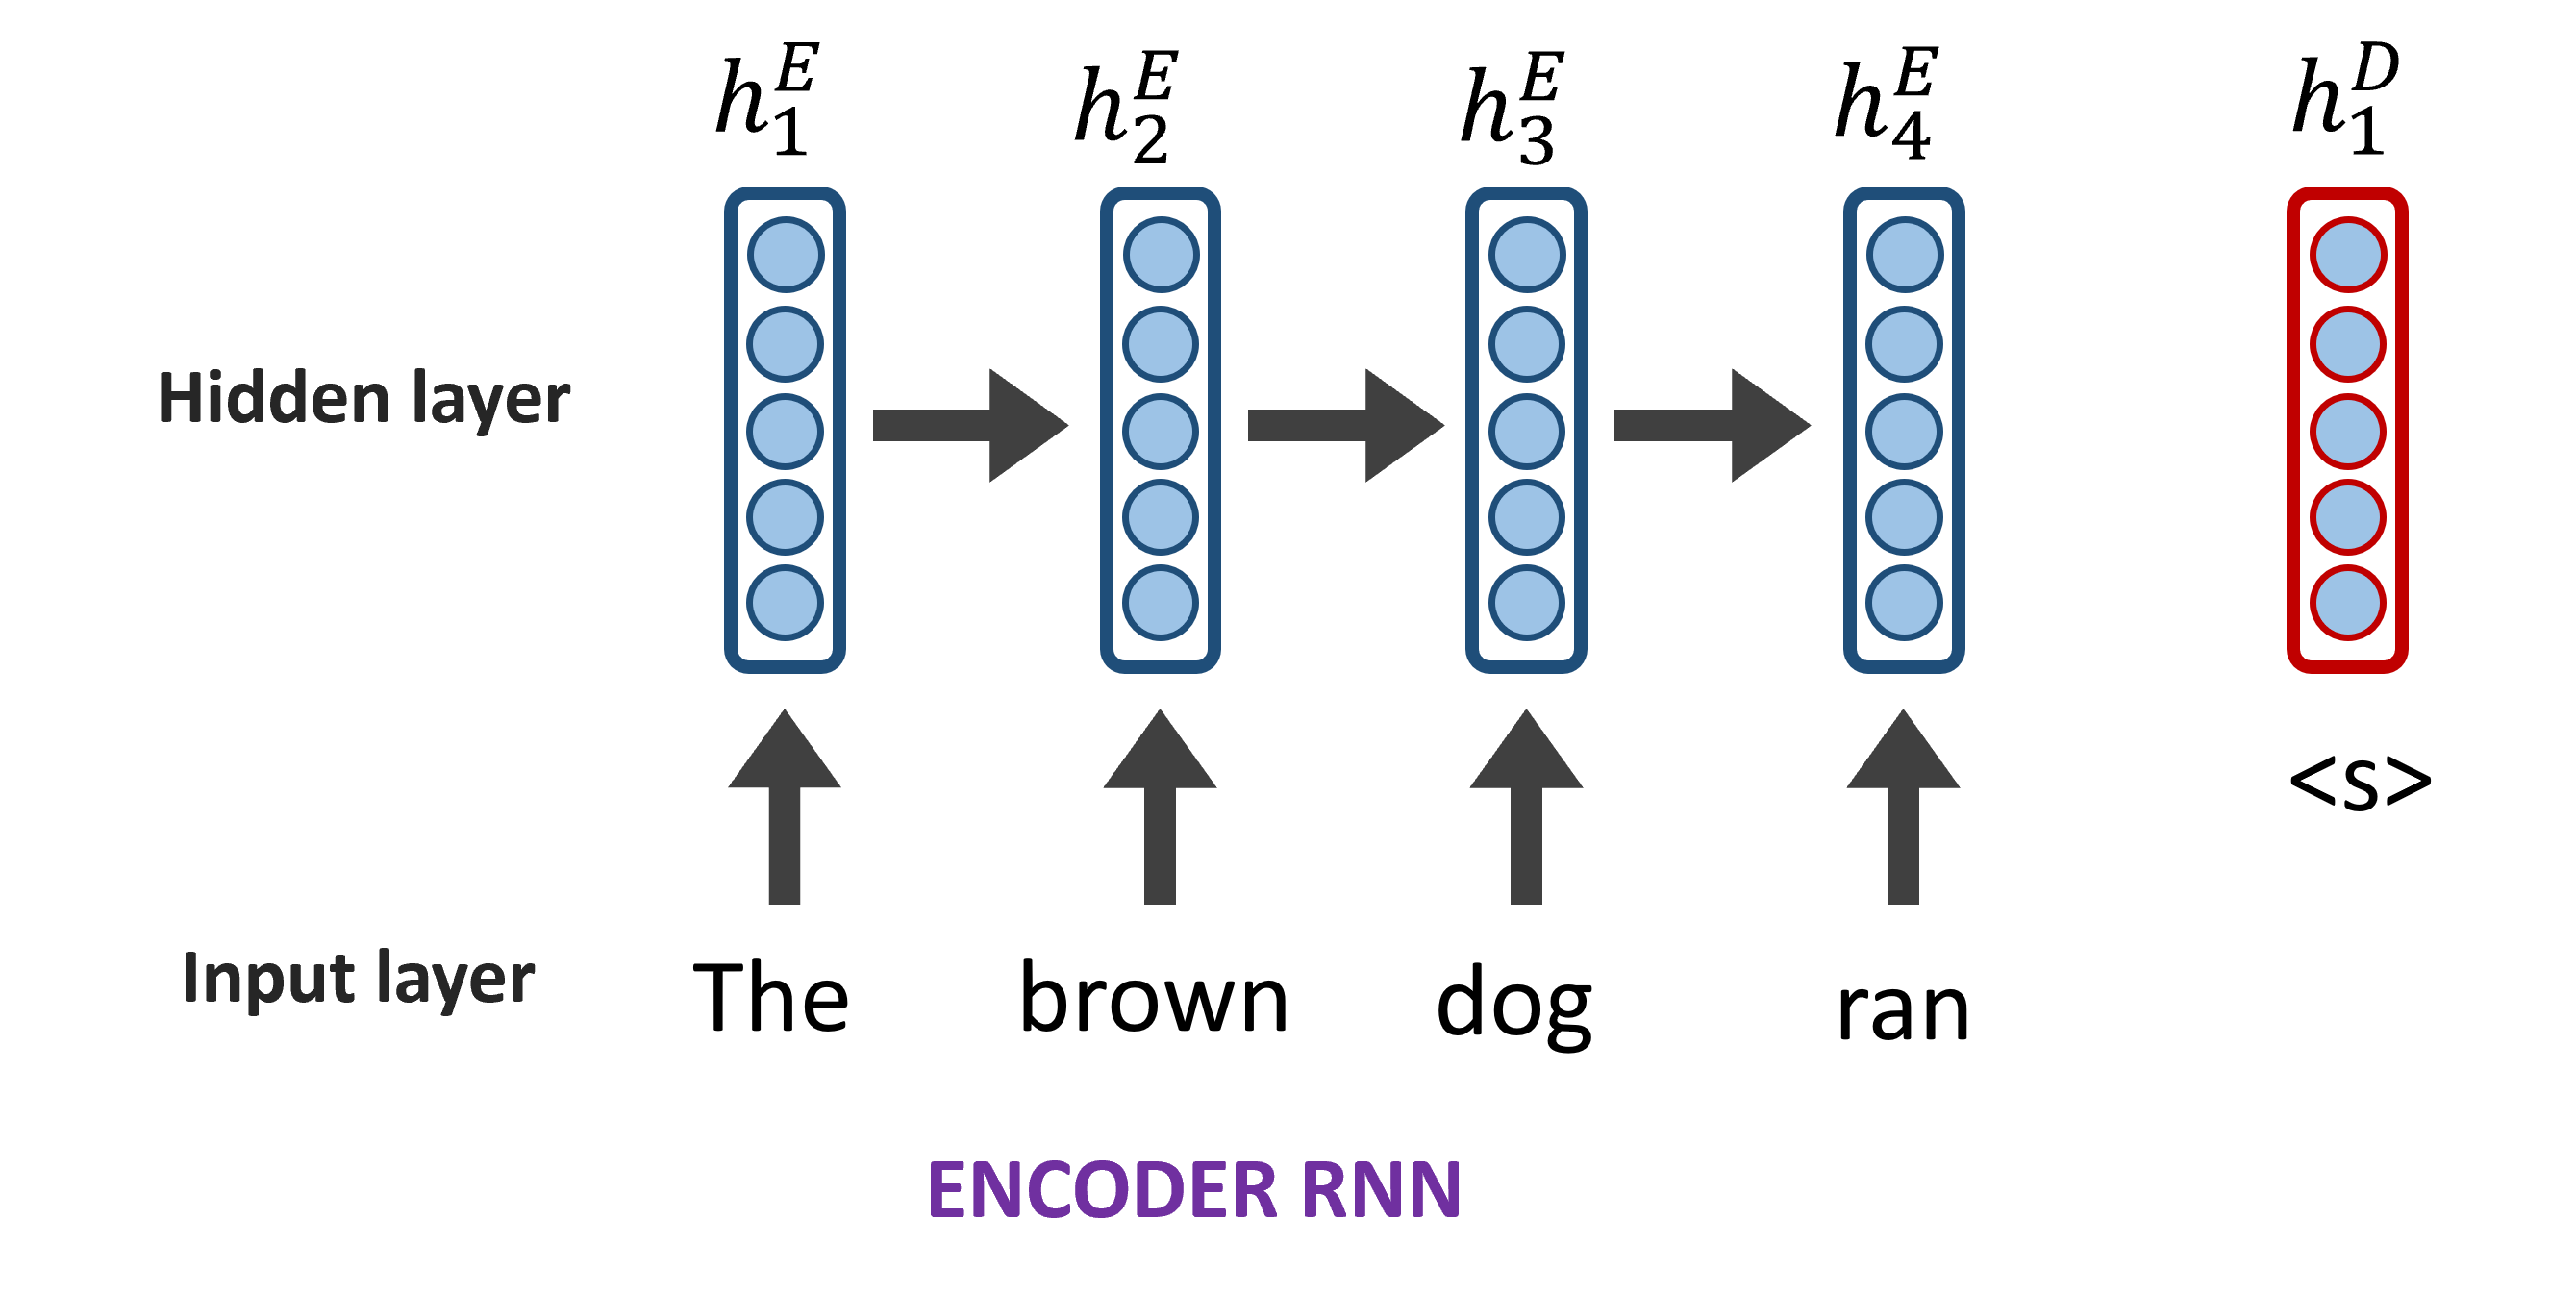
\includegraphics[width=0.8\linewidth,keepaspectratio]{bert17}
\end{center}	

\end{frame}

%%%%%%%%%%%%%%%%%%%%%%%%%%%%%%%%%%%%%%%%%%%%%%%%%%%%%%%%%%%
\begin{frame}[fragile]\frametitle{seq2seq + Attention}

Q: How do we determine how much to pay attention to each of the encoder’s hidden layers? 

A: Let’s base it on our decoder’s previous hidden state (our latest representation of meaning) and all of the encoder’s hidden layers! We want to measure similarity between decoder hidden state and encoder hidden stateS in some ways. 



\begin{center}
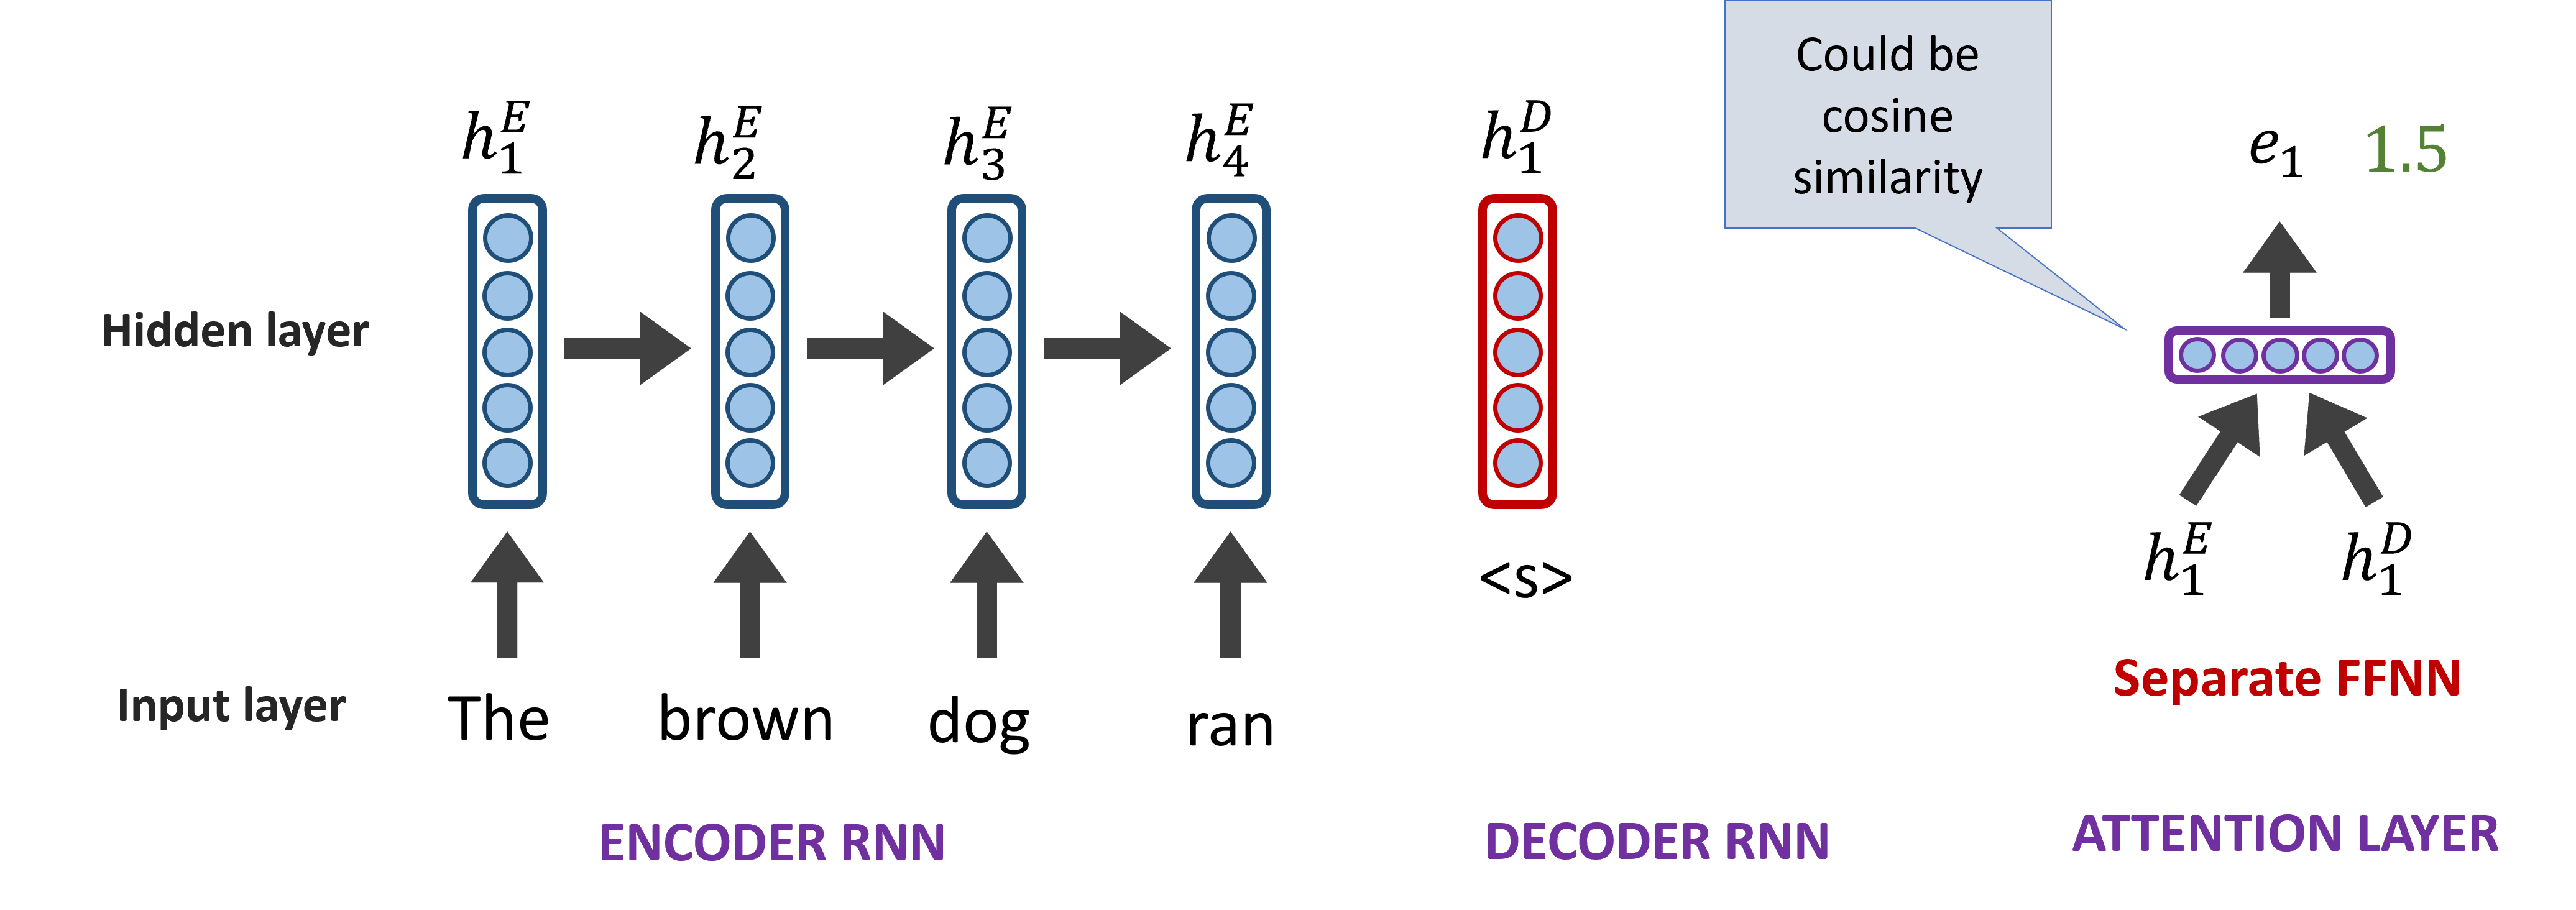
\includegraphics[width=0.8\linewidth,keepaspectratio]{bert18}
\end{center}	

\end{frame}

%%%%%%%%%%%%%%%%%%%%%%%%%%%%%%%%%%%%%%%%%%%%%%%%%%%%%%%%%%%
\begin{frame}[fragile]\frametitle{seq2seq + Attention}

Q: How do we determine how much to pay attention to each of the encoder’s hidden layers? 

A: Let’s base it on our decoder’s previous hidden state (our latest representation of meaning) and all of the encoder’s hidden layers! We want to measure similarity between decoder hidden state and encoder hidden stateS in some ways. 



\begin{center}
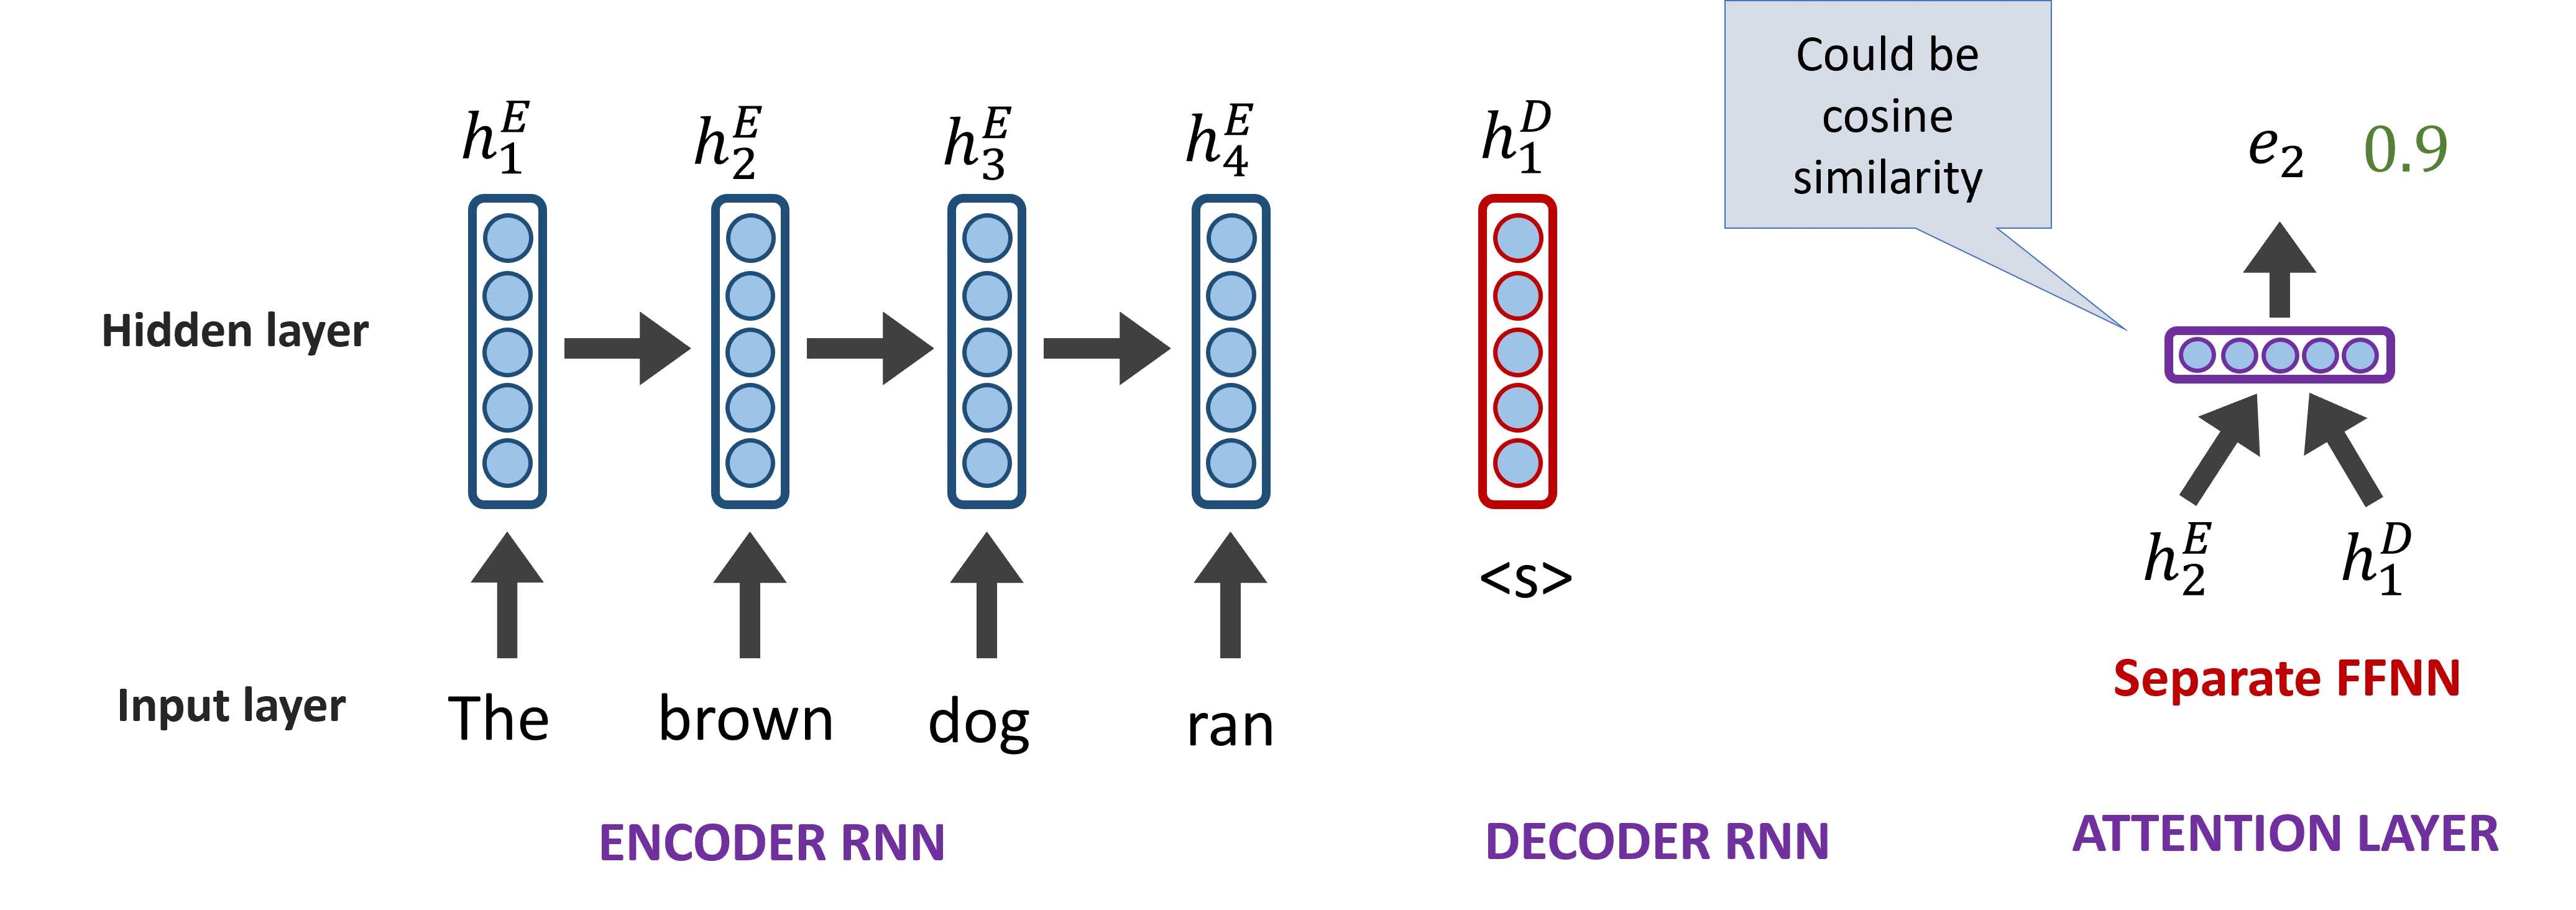
\includegraphics[width=0.8\linewidth,keepaspectratio]{bert19}
\end{center}	

\end{frame}

%%%%%%%%%%%%%%%%%%%%%%%%%%%%%%%%%%%%%%%%%%%%%%%%%%%%%%%%%%%
\begin{frame}[fragile]\frametitle{seq2seq + Attention}

Q: How do we determine how much to pay attention to each of the encoder’s hidden layers? 

A: Let’s base it on our decoder’s previous hidden state (our latest representation of meaning) and all of the encoder’s hidden layers! We want to measure similarity between decoder hidden state and encoder hidden stateS in some ways. 



\begin{center}
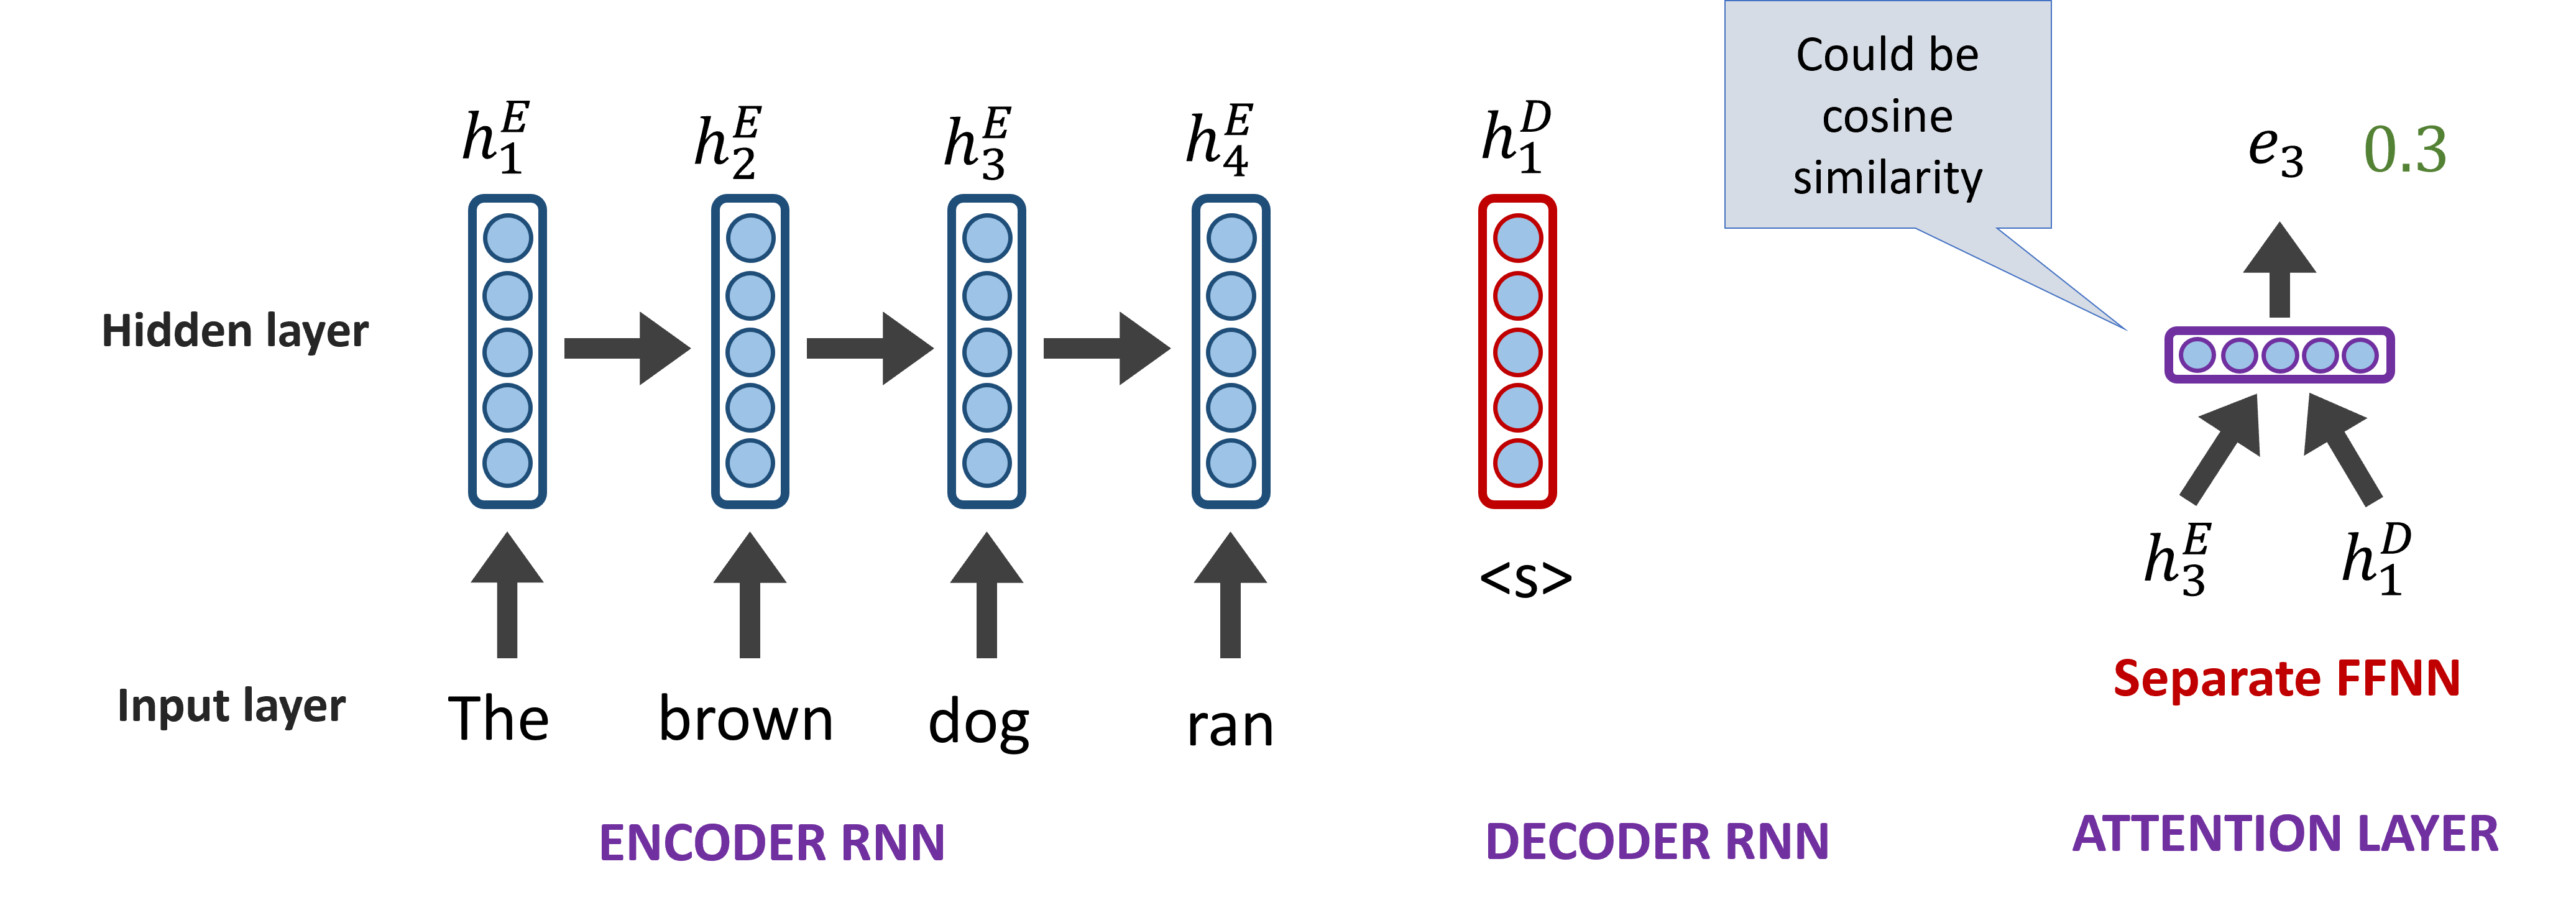
\includegraphics[width=0.8\linewidth,keepaspectratio]{bert20}
\end{center}	

\end{frame}

%%%%%%%%%%%%%%%%%%%%%%%%%%%%%%%%%%%%%%%%%%%%%%%%%%%%%%%%%%%
\begin{frame}[fragile]\frametitle{seq2seq + Attention}

Q: How do we determine how much to pay attention to each of the encoder’s hidden layers? 

A: Let’s base it on our decoder’s previous hidden state (our latest representation of meaning) and all of the encoder’s hidden layers! We want to measure similarity between decoder hidden state and encoder hidden stateS in some ways. 



\begin{center}
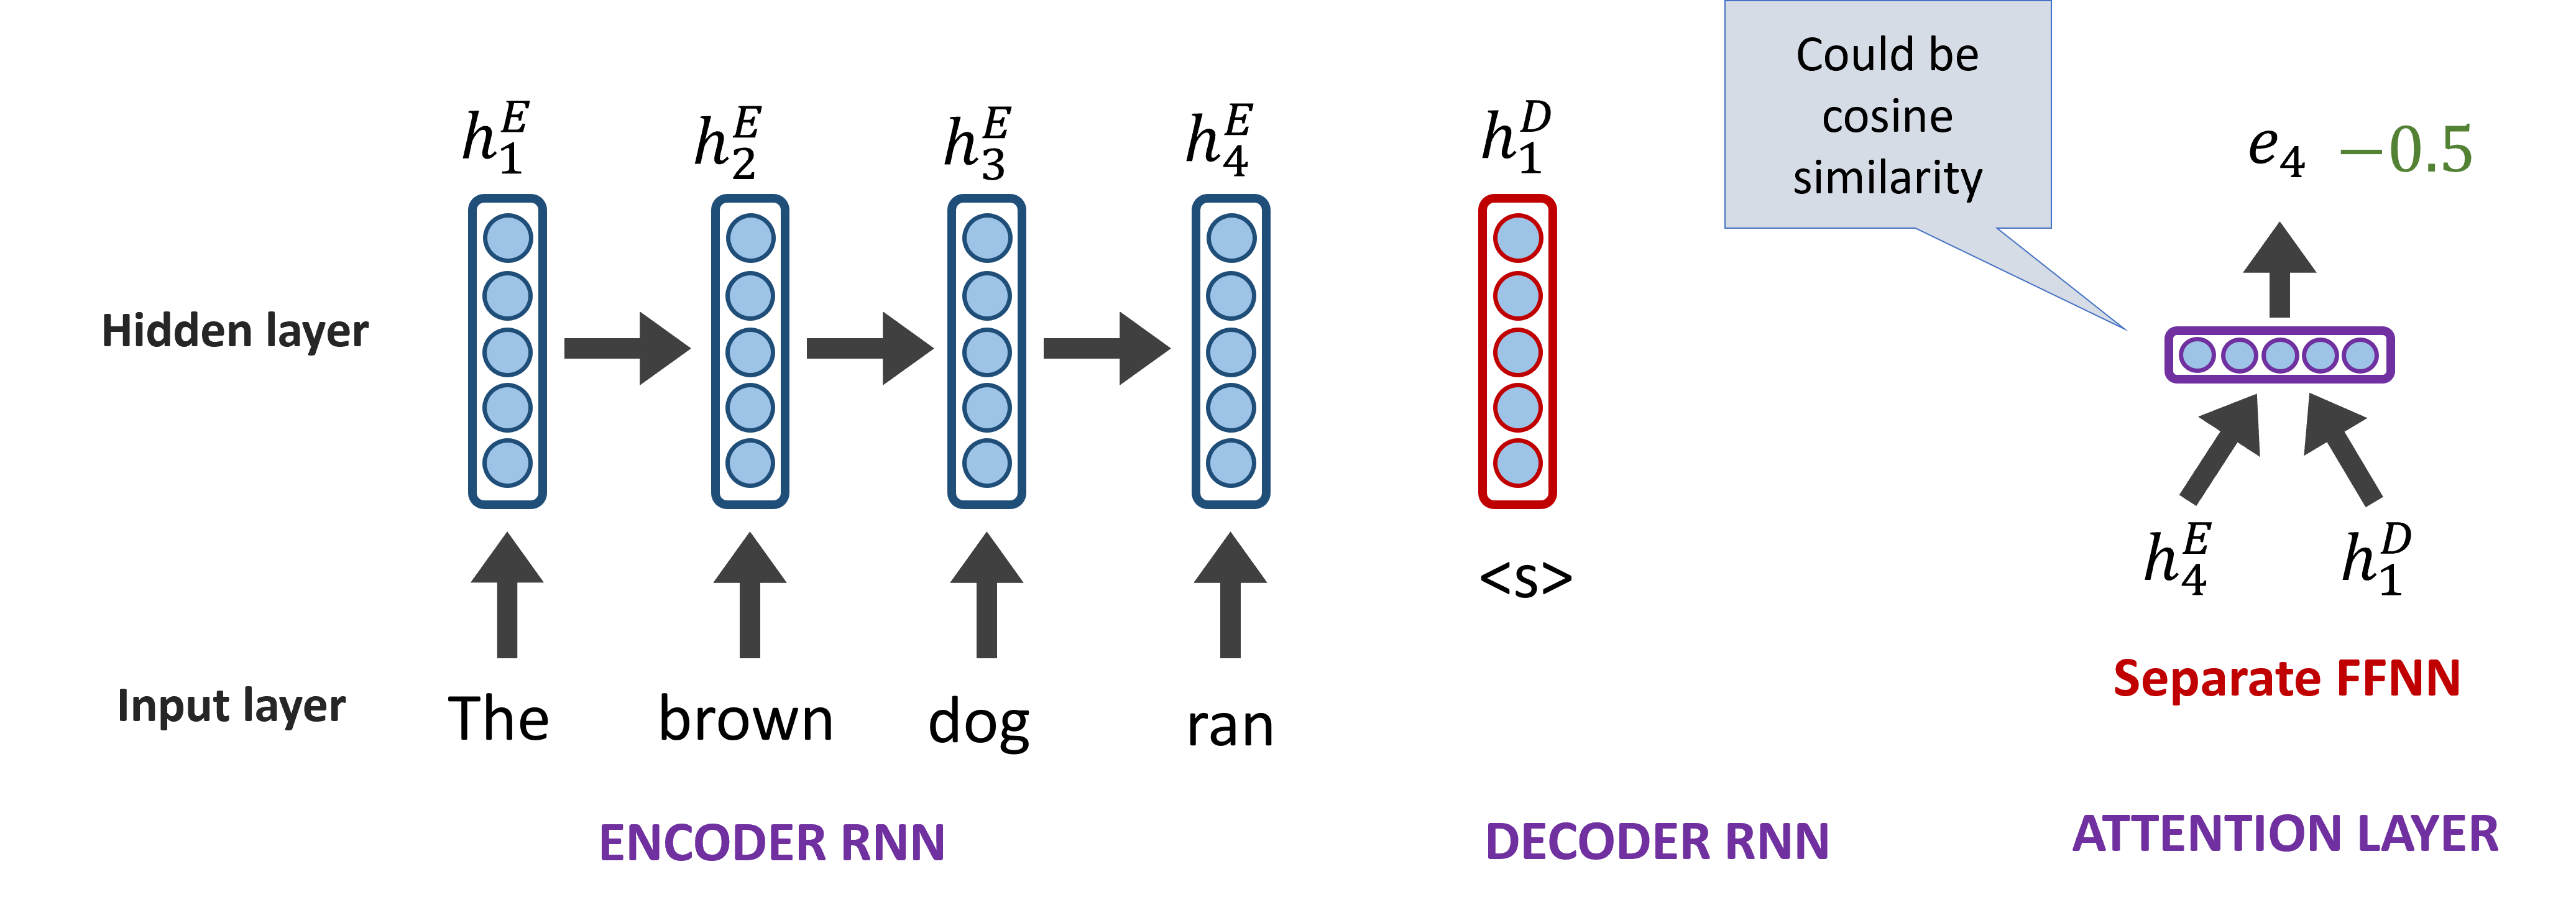
\includegraphics[width=0.8\linewidth,keepaspectratio]{bert21}
\end{center}	

\end{frame}

%%%%%%%%%%%%%%%%%%%%%%%%%%%%%%%%%%%%%%%%%%%%%%%%%%%%%%%%%%%
\begin{frame}[fragile]\frametitle{seq2seq + Attention}

Q: How do we determine how much to pay attention to each of the encoder’s hidden layers? 

A: Let’s base it on our decoder’s previous hidden state (our latest representation of meaning) and all of the encoder’s hidden layers!



\begin{center}
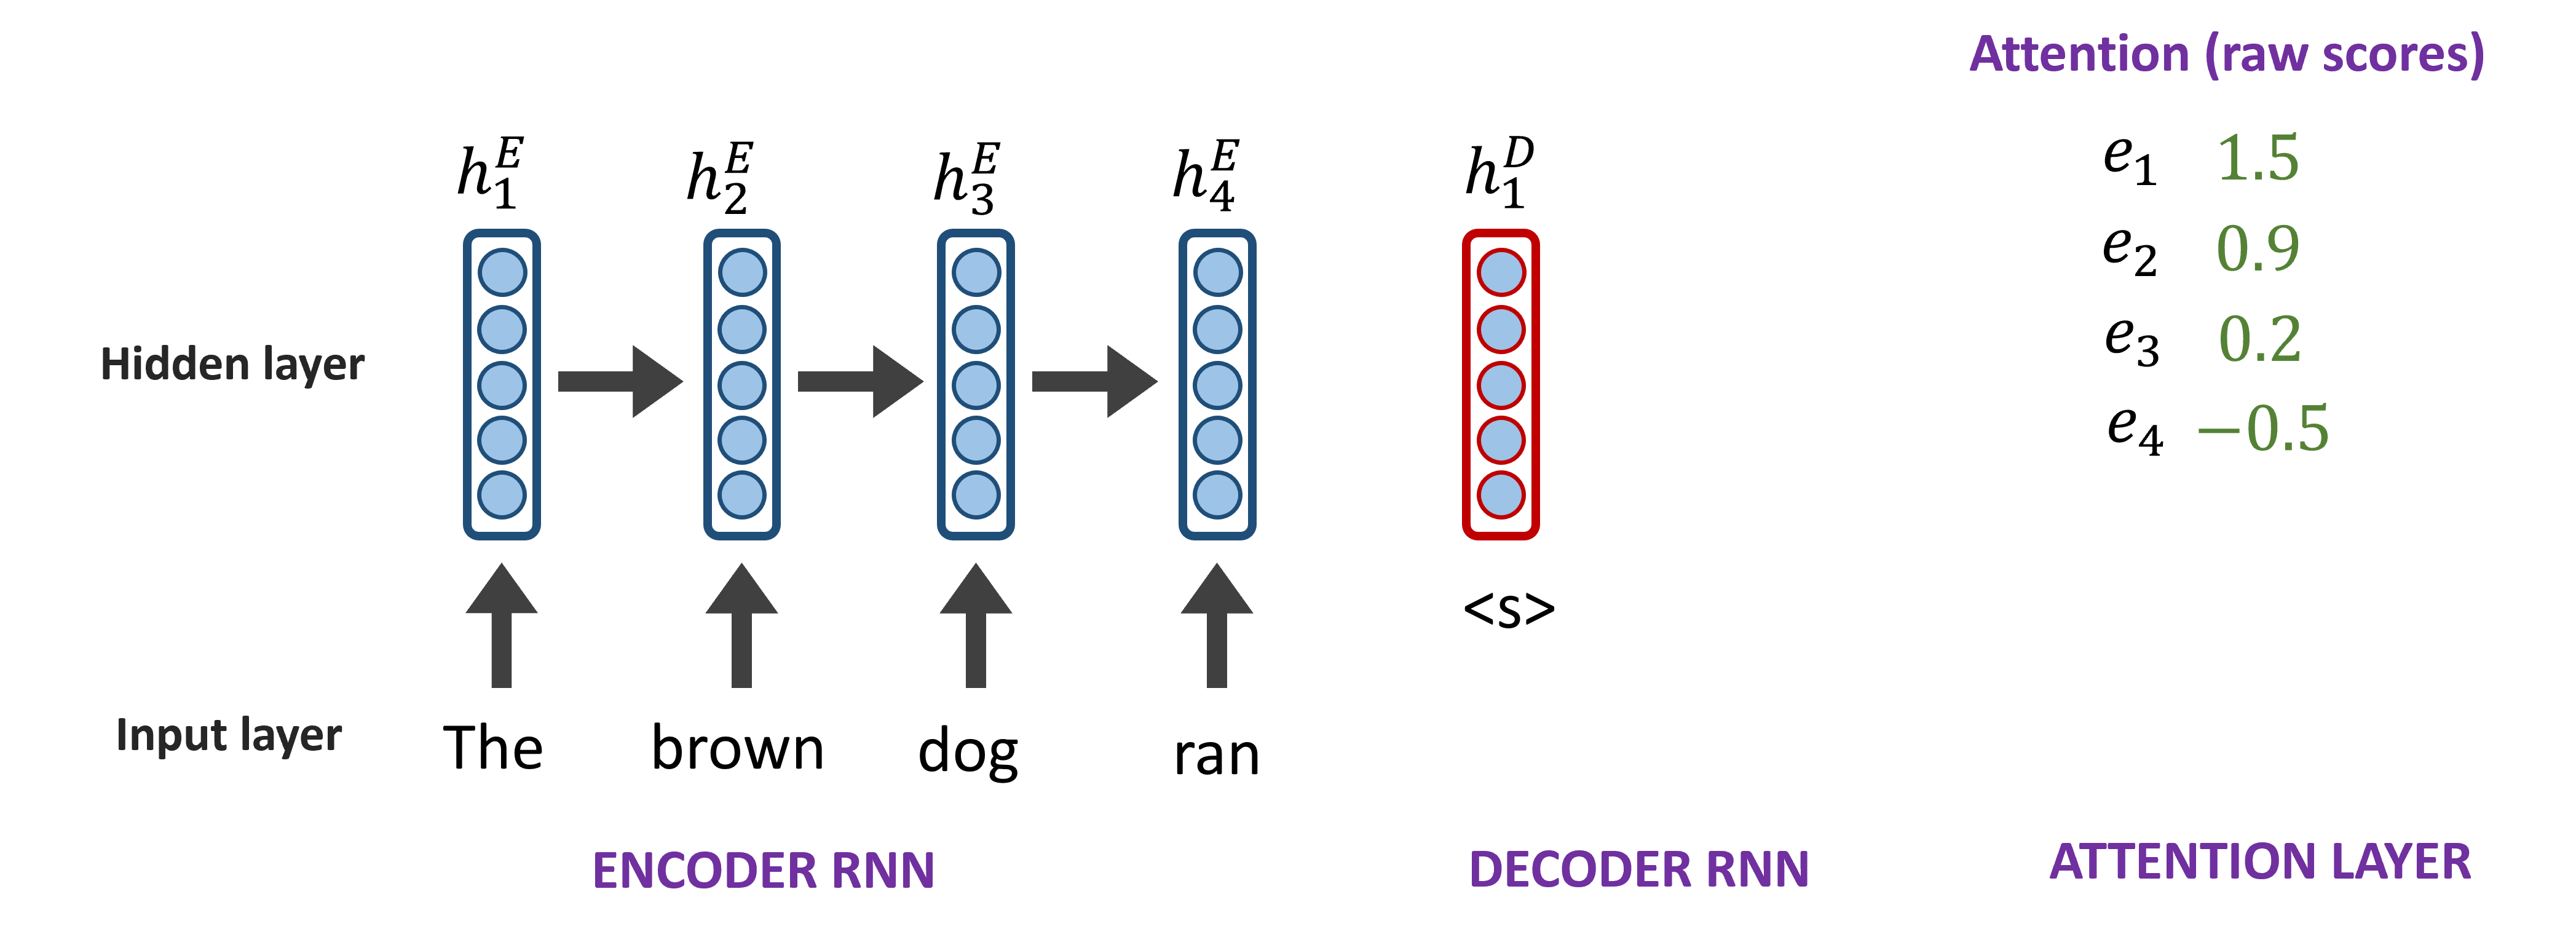
\includegraphics[width=0.8\linewidth,keepaspectratio]{bert22}
\end{center}	

\end{frame}

%%%%%%%%%%%%%%%%%%%%%%%%%%%%%%%%%%%%%%%%%%%%%%%%%%%%%%%%%%%
\begin{frame}[fragile]\frametitle{seq2seq + Attention}

Q: How do we determine how much to pay attention to each of the encoder’s hidden layers? 

A: Let’s base it on our decoder’s previous hidden state (our latest representation of meaning) and all of the encoder’s hidden layers!



\begin{center}
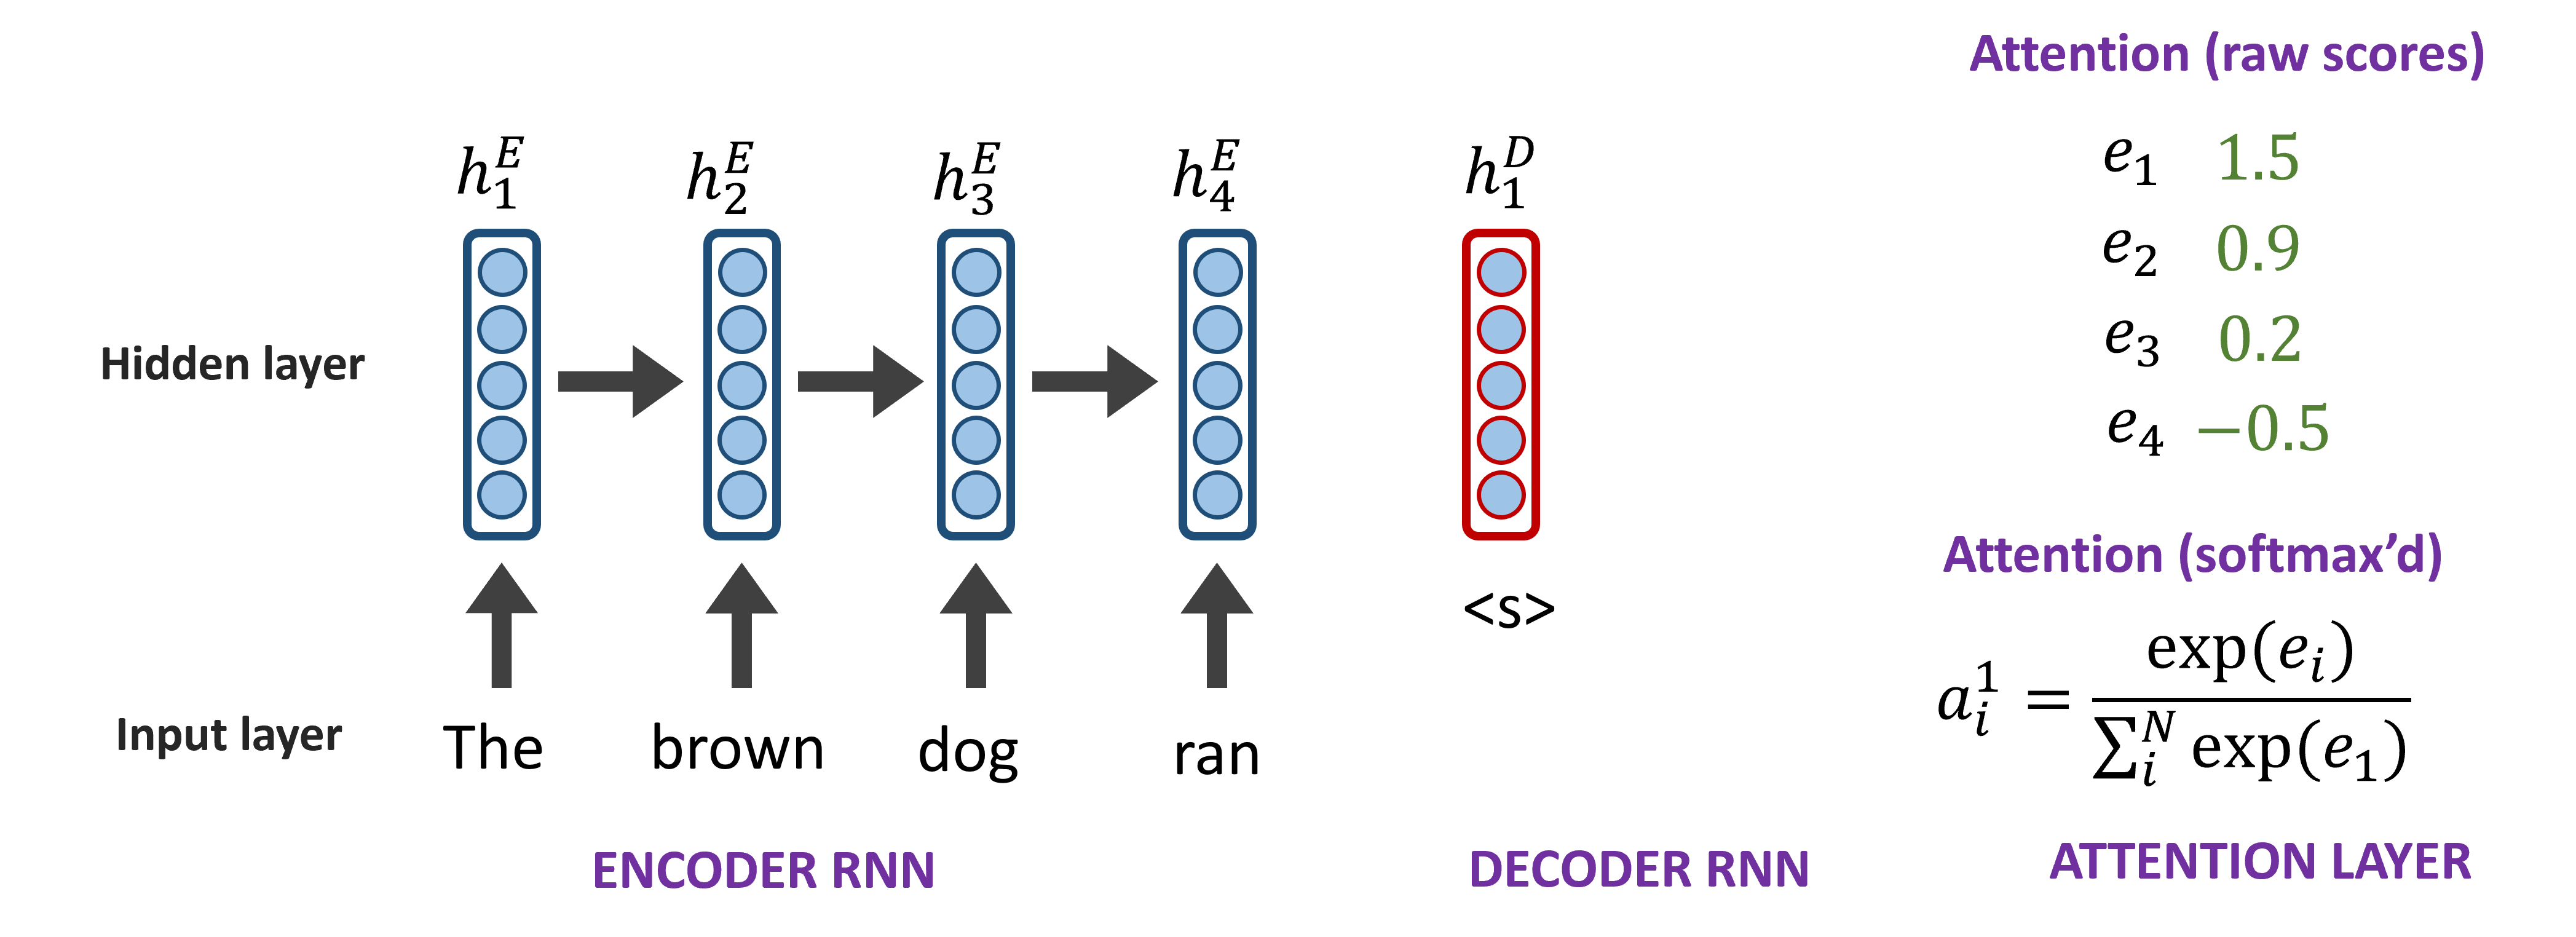
\includegraphics[width=0.8\linewidth,keepaspectratio]{bert23}
\end{center}	

\end{frame}

%%%%%%%%%%%%%%%%%%%%%%%%%%%%%%%%%%%%%%%%%%%%%%%%%%%%%%%%%%%
\begin{frame}[fragile]\frametitle{seq2seq + Attention}

Q: How do we determine how much to pay attention to each of the encoder’s hidden layers? 

A: Let’s base it on our decoder’s previous hidden state (our latest representation of meaning) and all of the encoder’s hidden layers!



\begin{center}
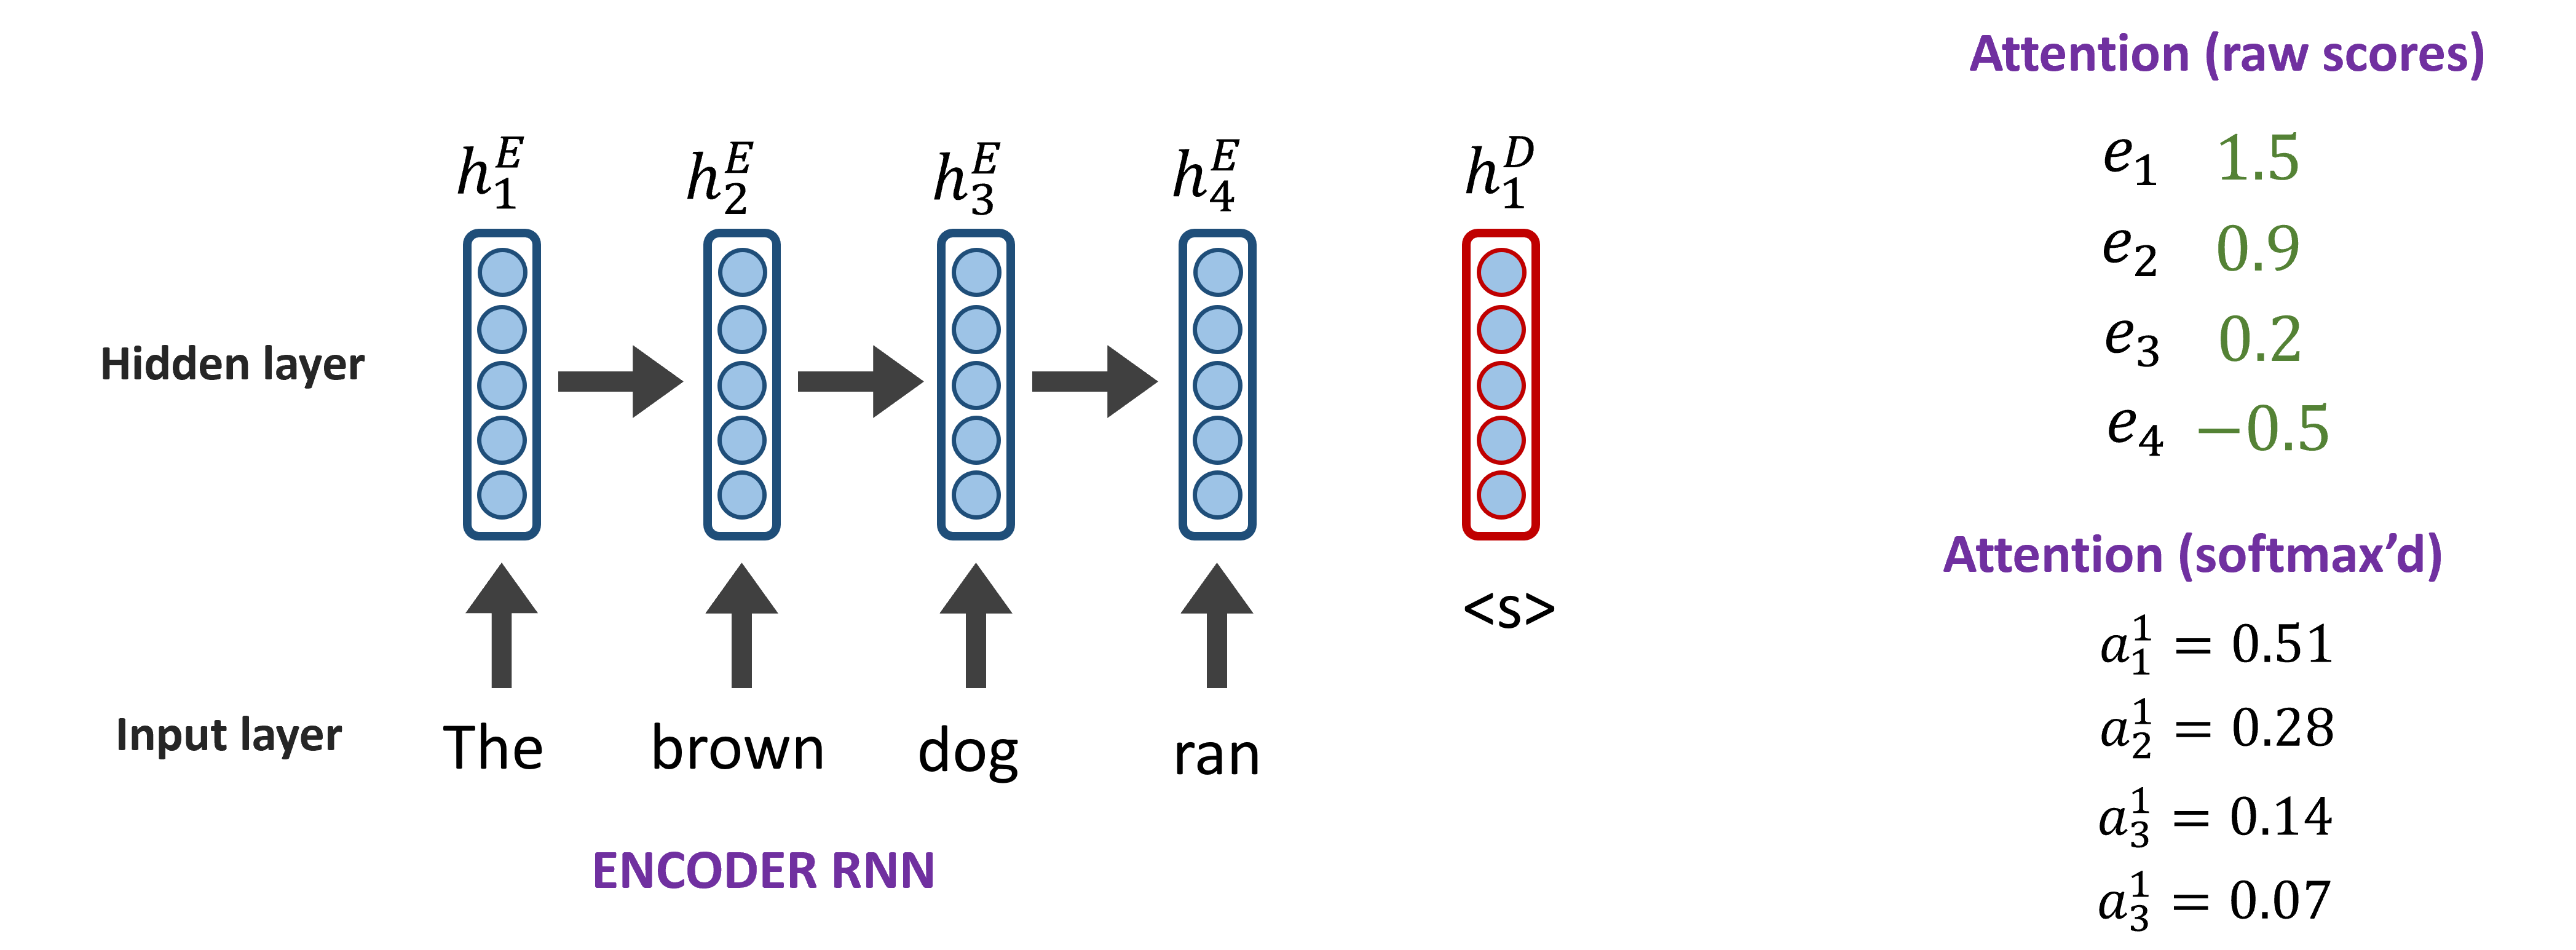
\includegraphics[width=0.8\linewidth,keepaspectratio]{bert24}
\end{center}	

\end{frame}

%%%%%%%%%%%%%%%%%%%%%%%%%%%%%%%%%%%%%%%%%%%%%%%%%%%%%%%%%%%
\begin{frame}[fragile]\frametitle{seq2seq + Attention}

\begin{center}
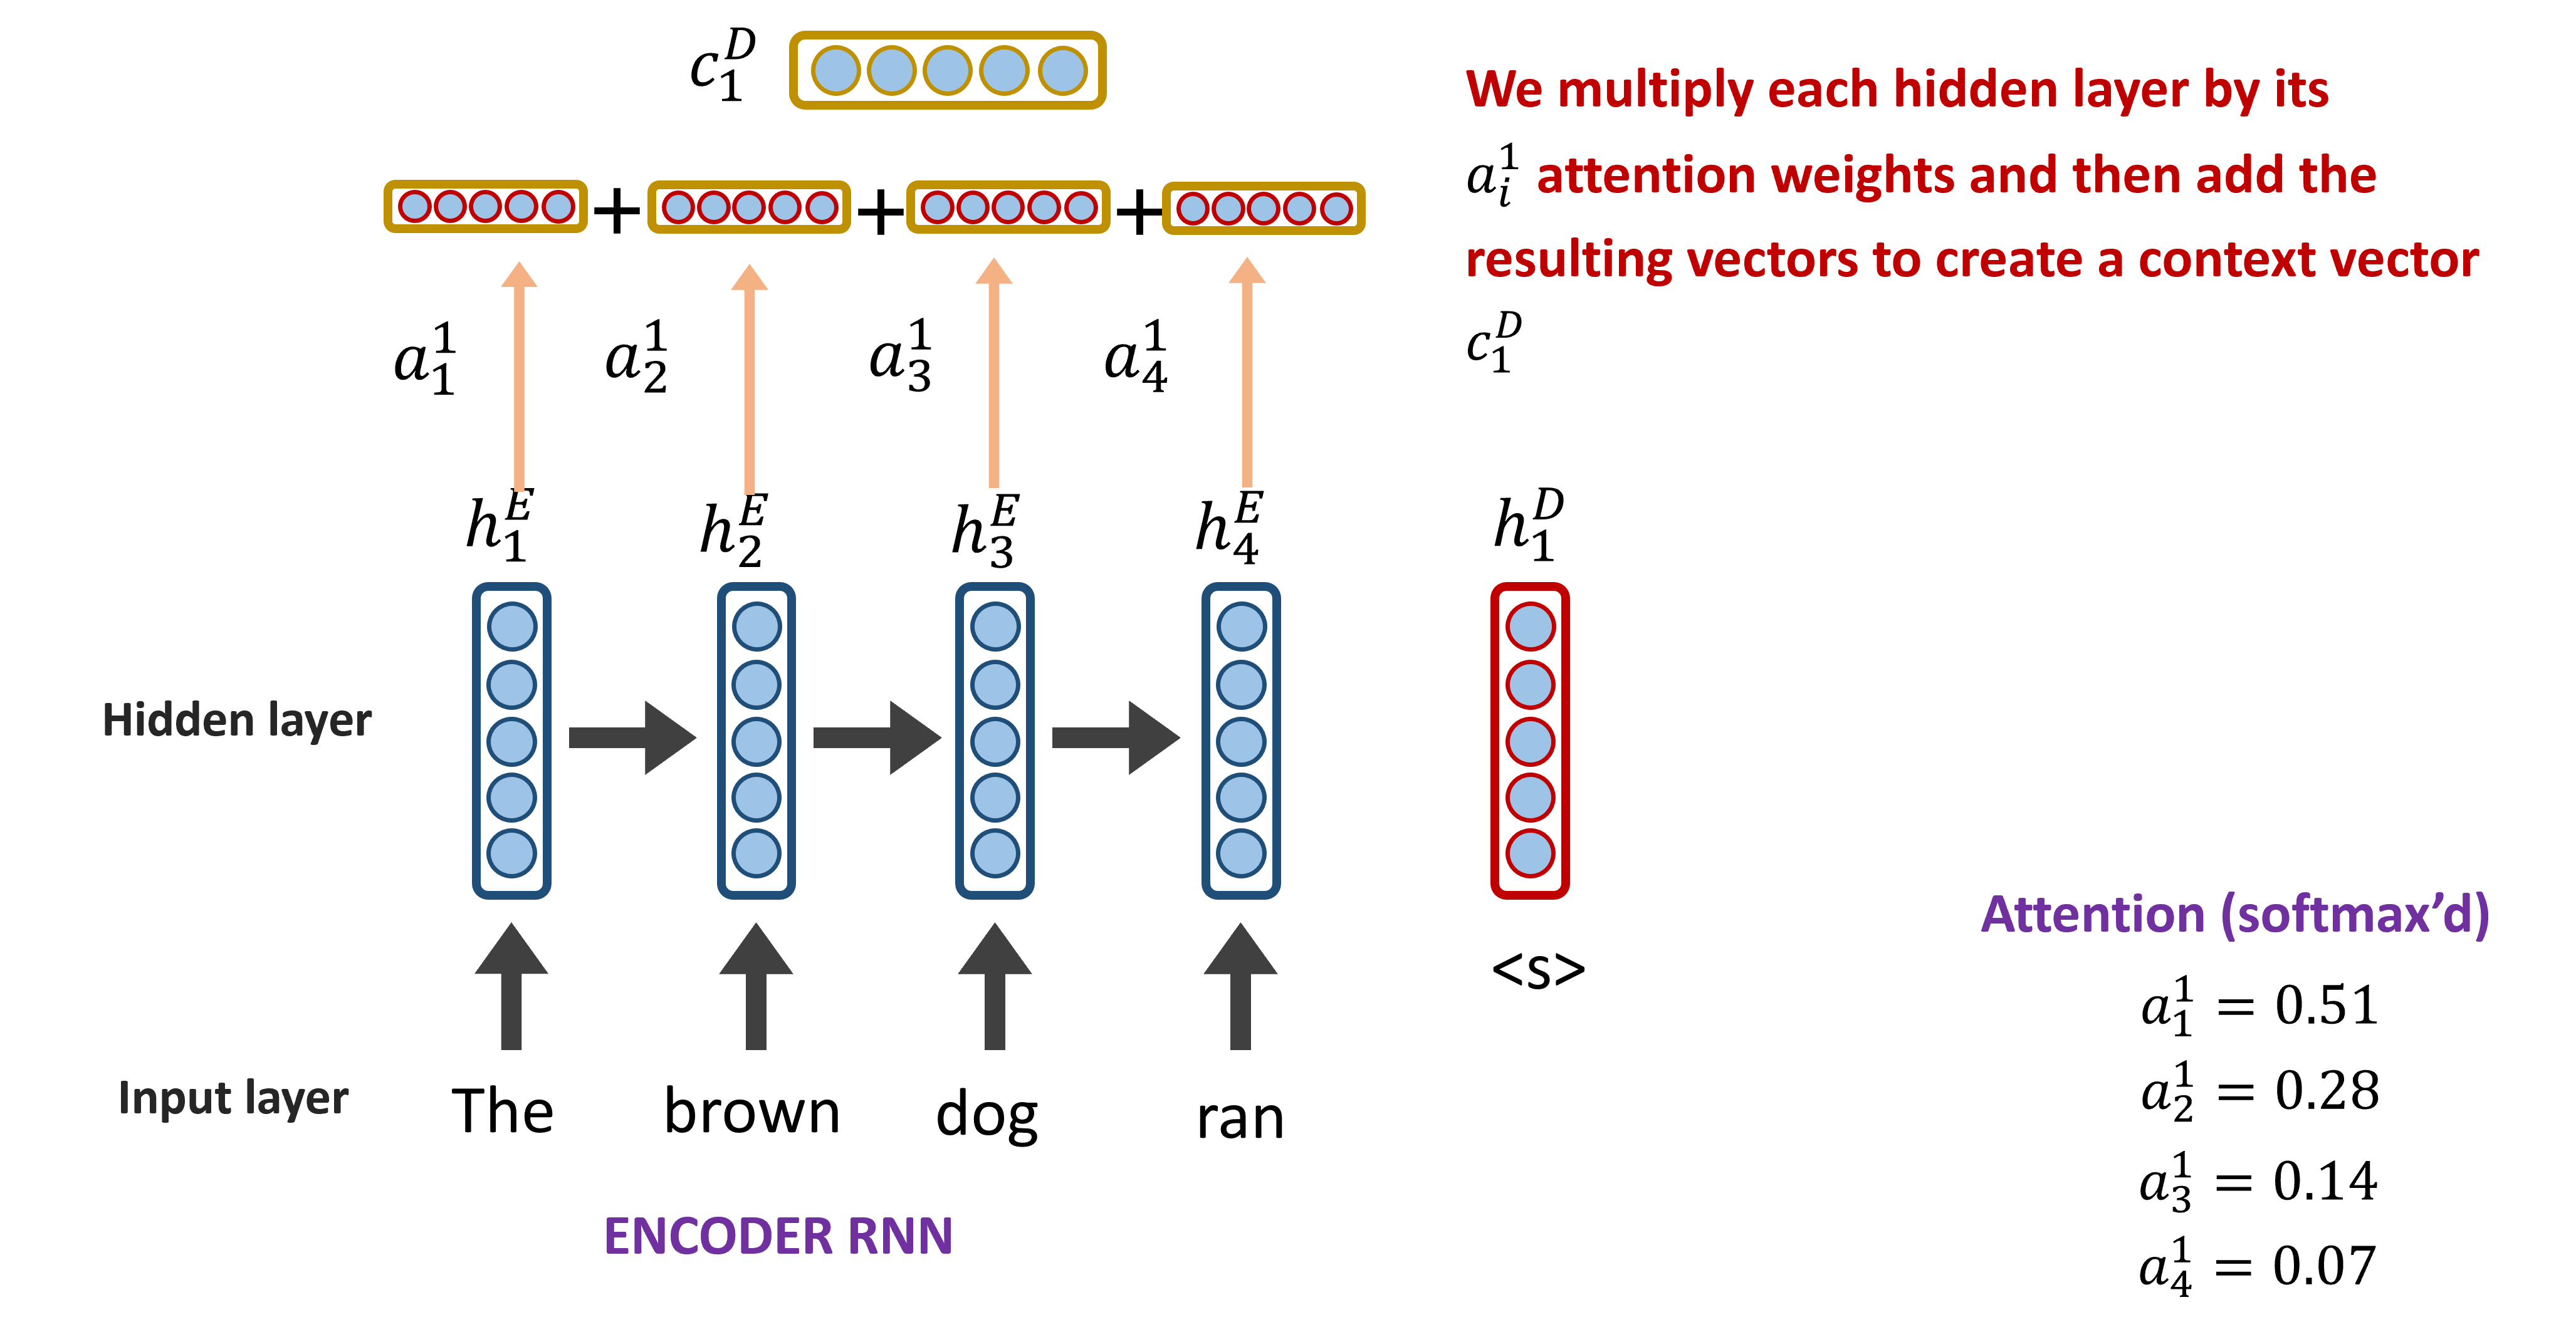
\includegraphics[width=0.8\linewidth,keepaspectratio]{bert25}
\end{center}	

\end{frame}

%%%%%%%%%%%%%%%%%%%%%%%%%%%%%%%%%%%%%%%%%%%%%%%%%%%%%%%%%%%
\begin{frame}[fragile]\frametitle{seq2seq + Attention}

\begin{center}
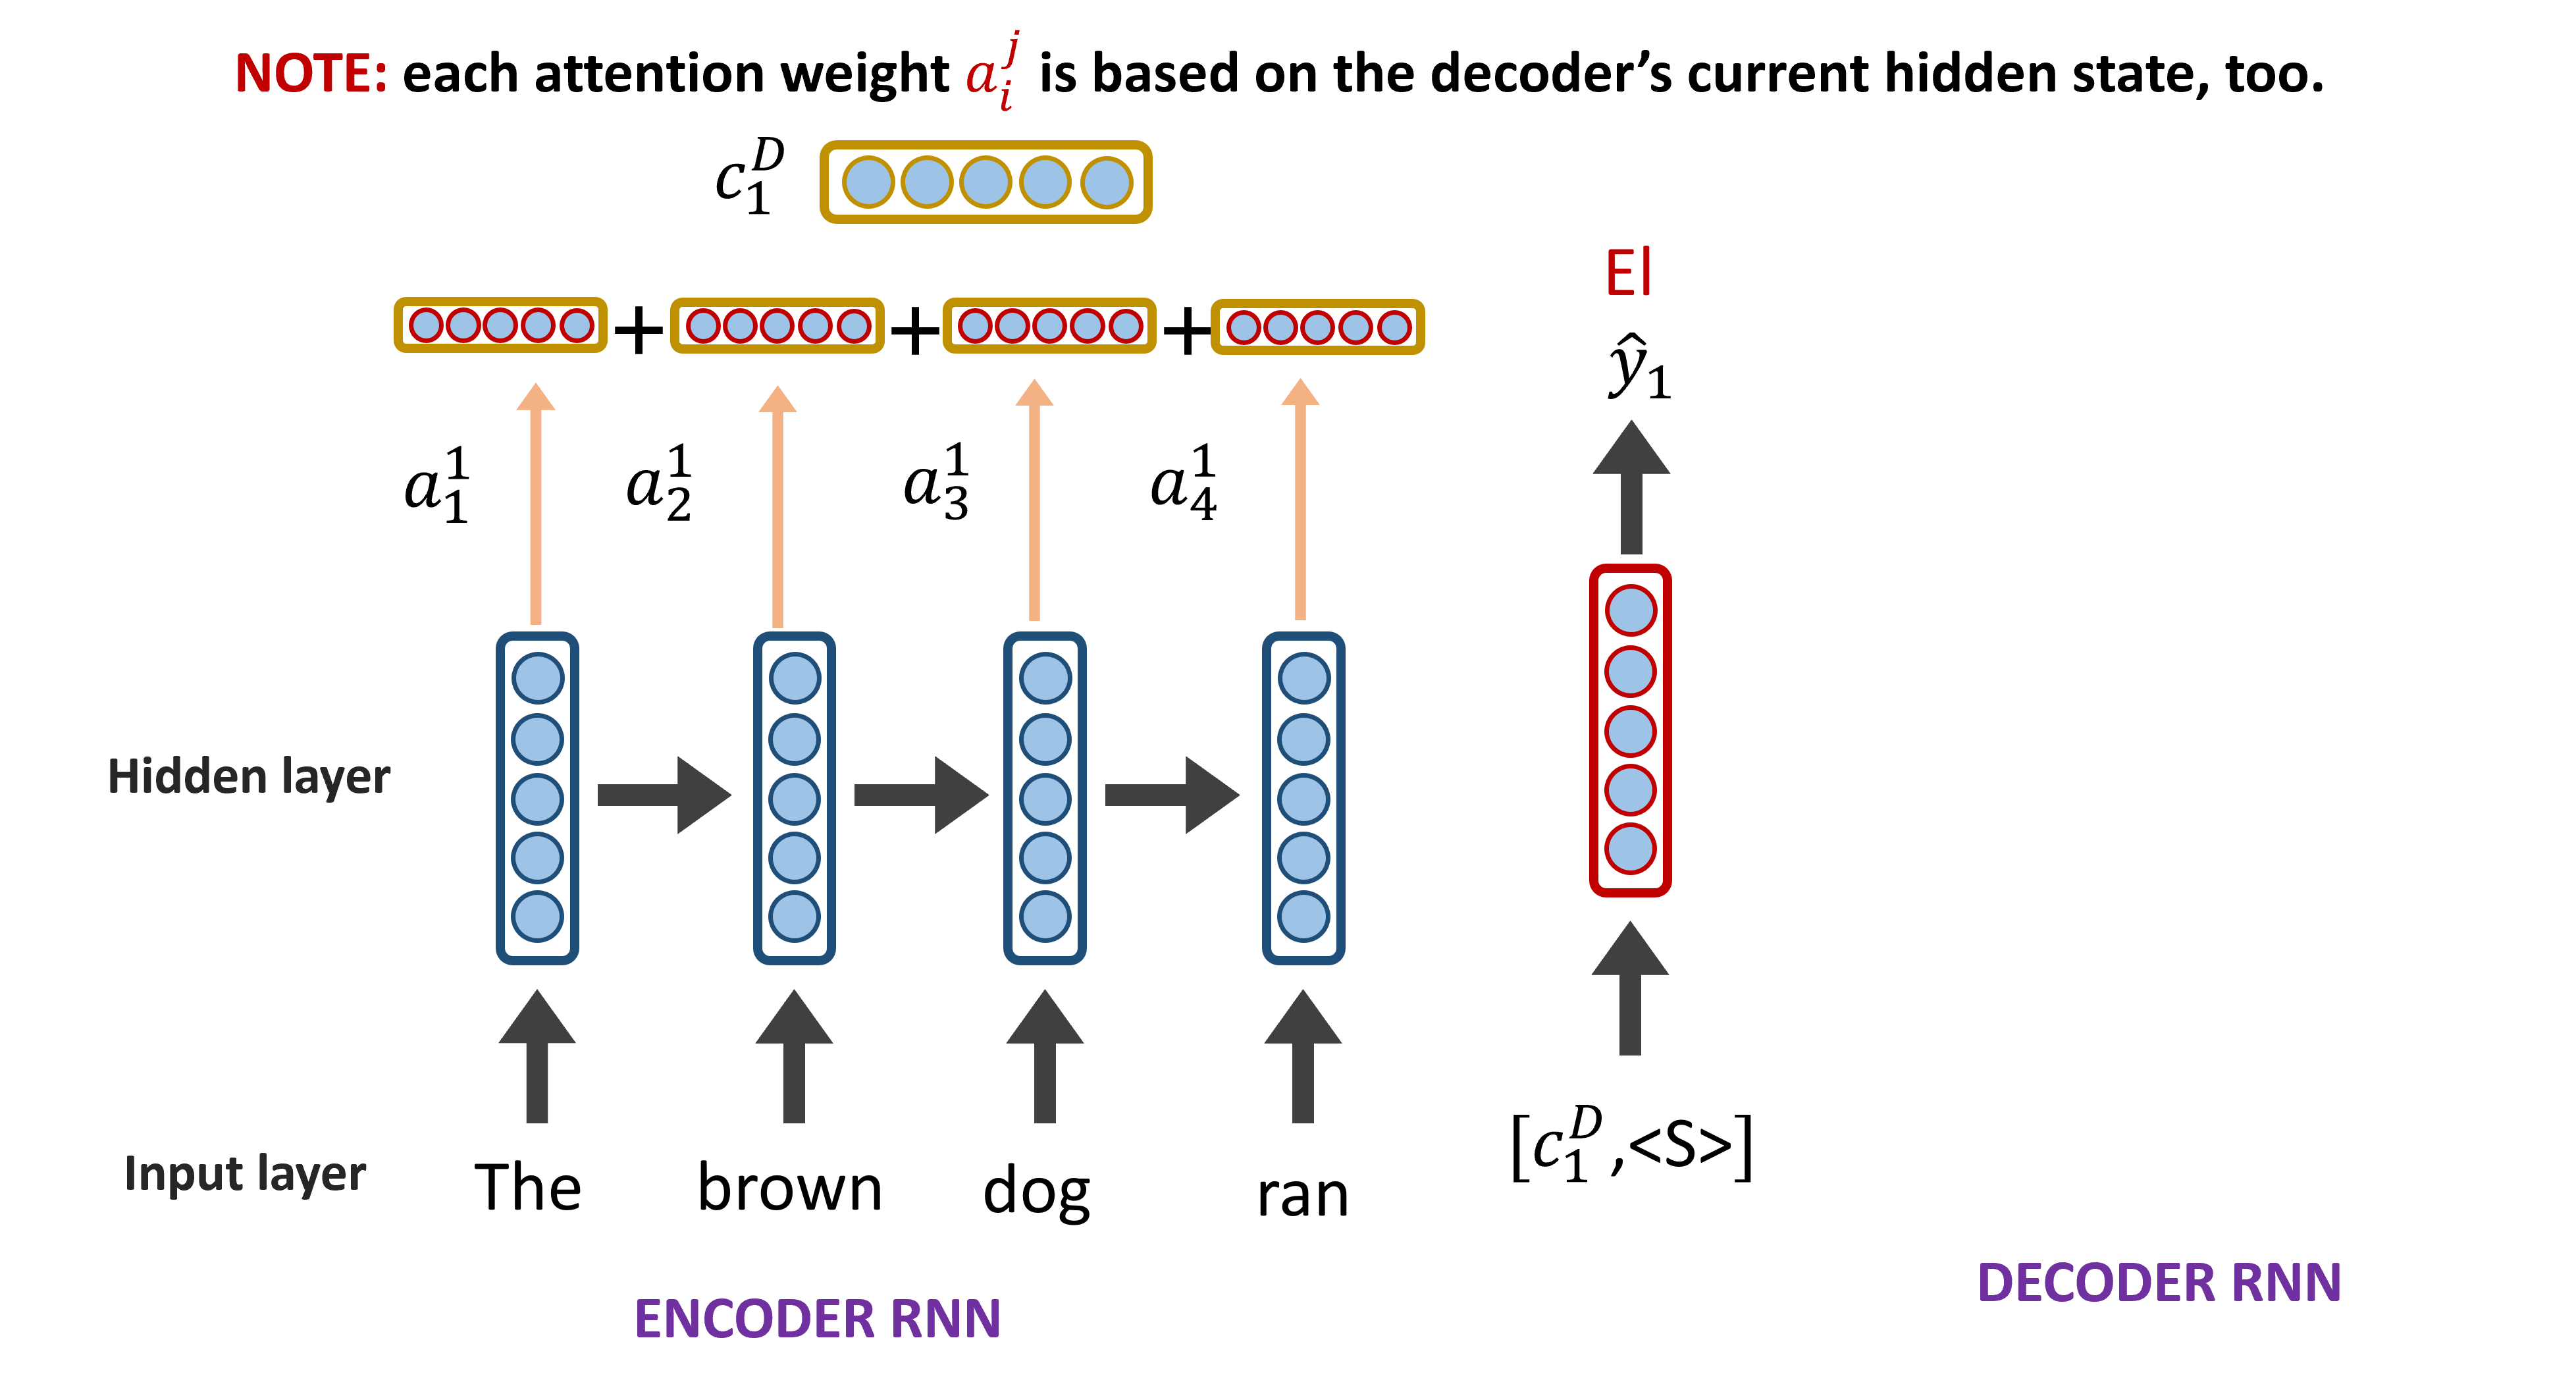
\includegraphics[width=0.8\linewidth,keepaspectratio]{bert26}
\end{center}	

\end{frame}

%%%%%%%%%%%%%%%%%%%%%%%%%%%%%%%%%%%%%%%%%%%%%%%%%%%%%%%%%%%
\begin{frame}[fragile]\frametitle{seq2seq + Attention}

\begin{center}
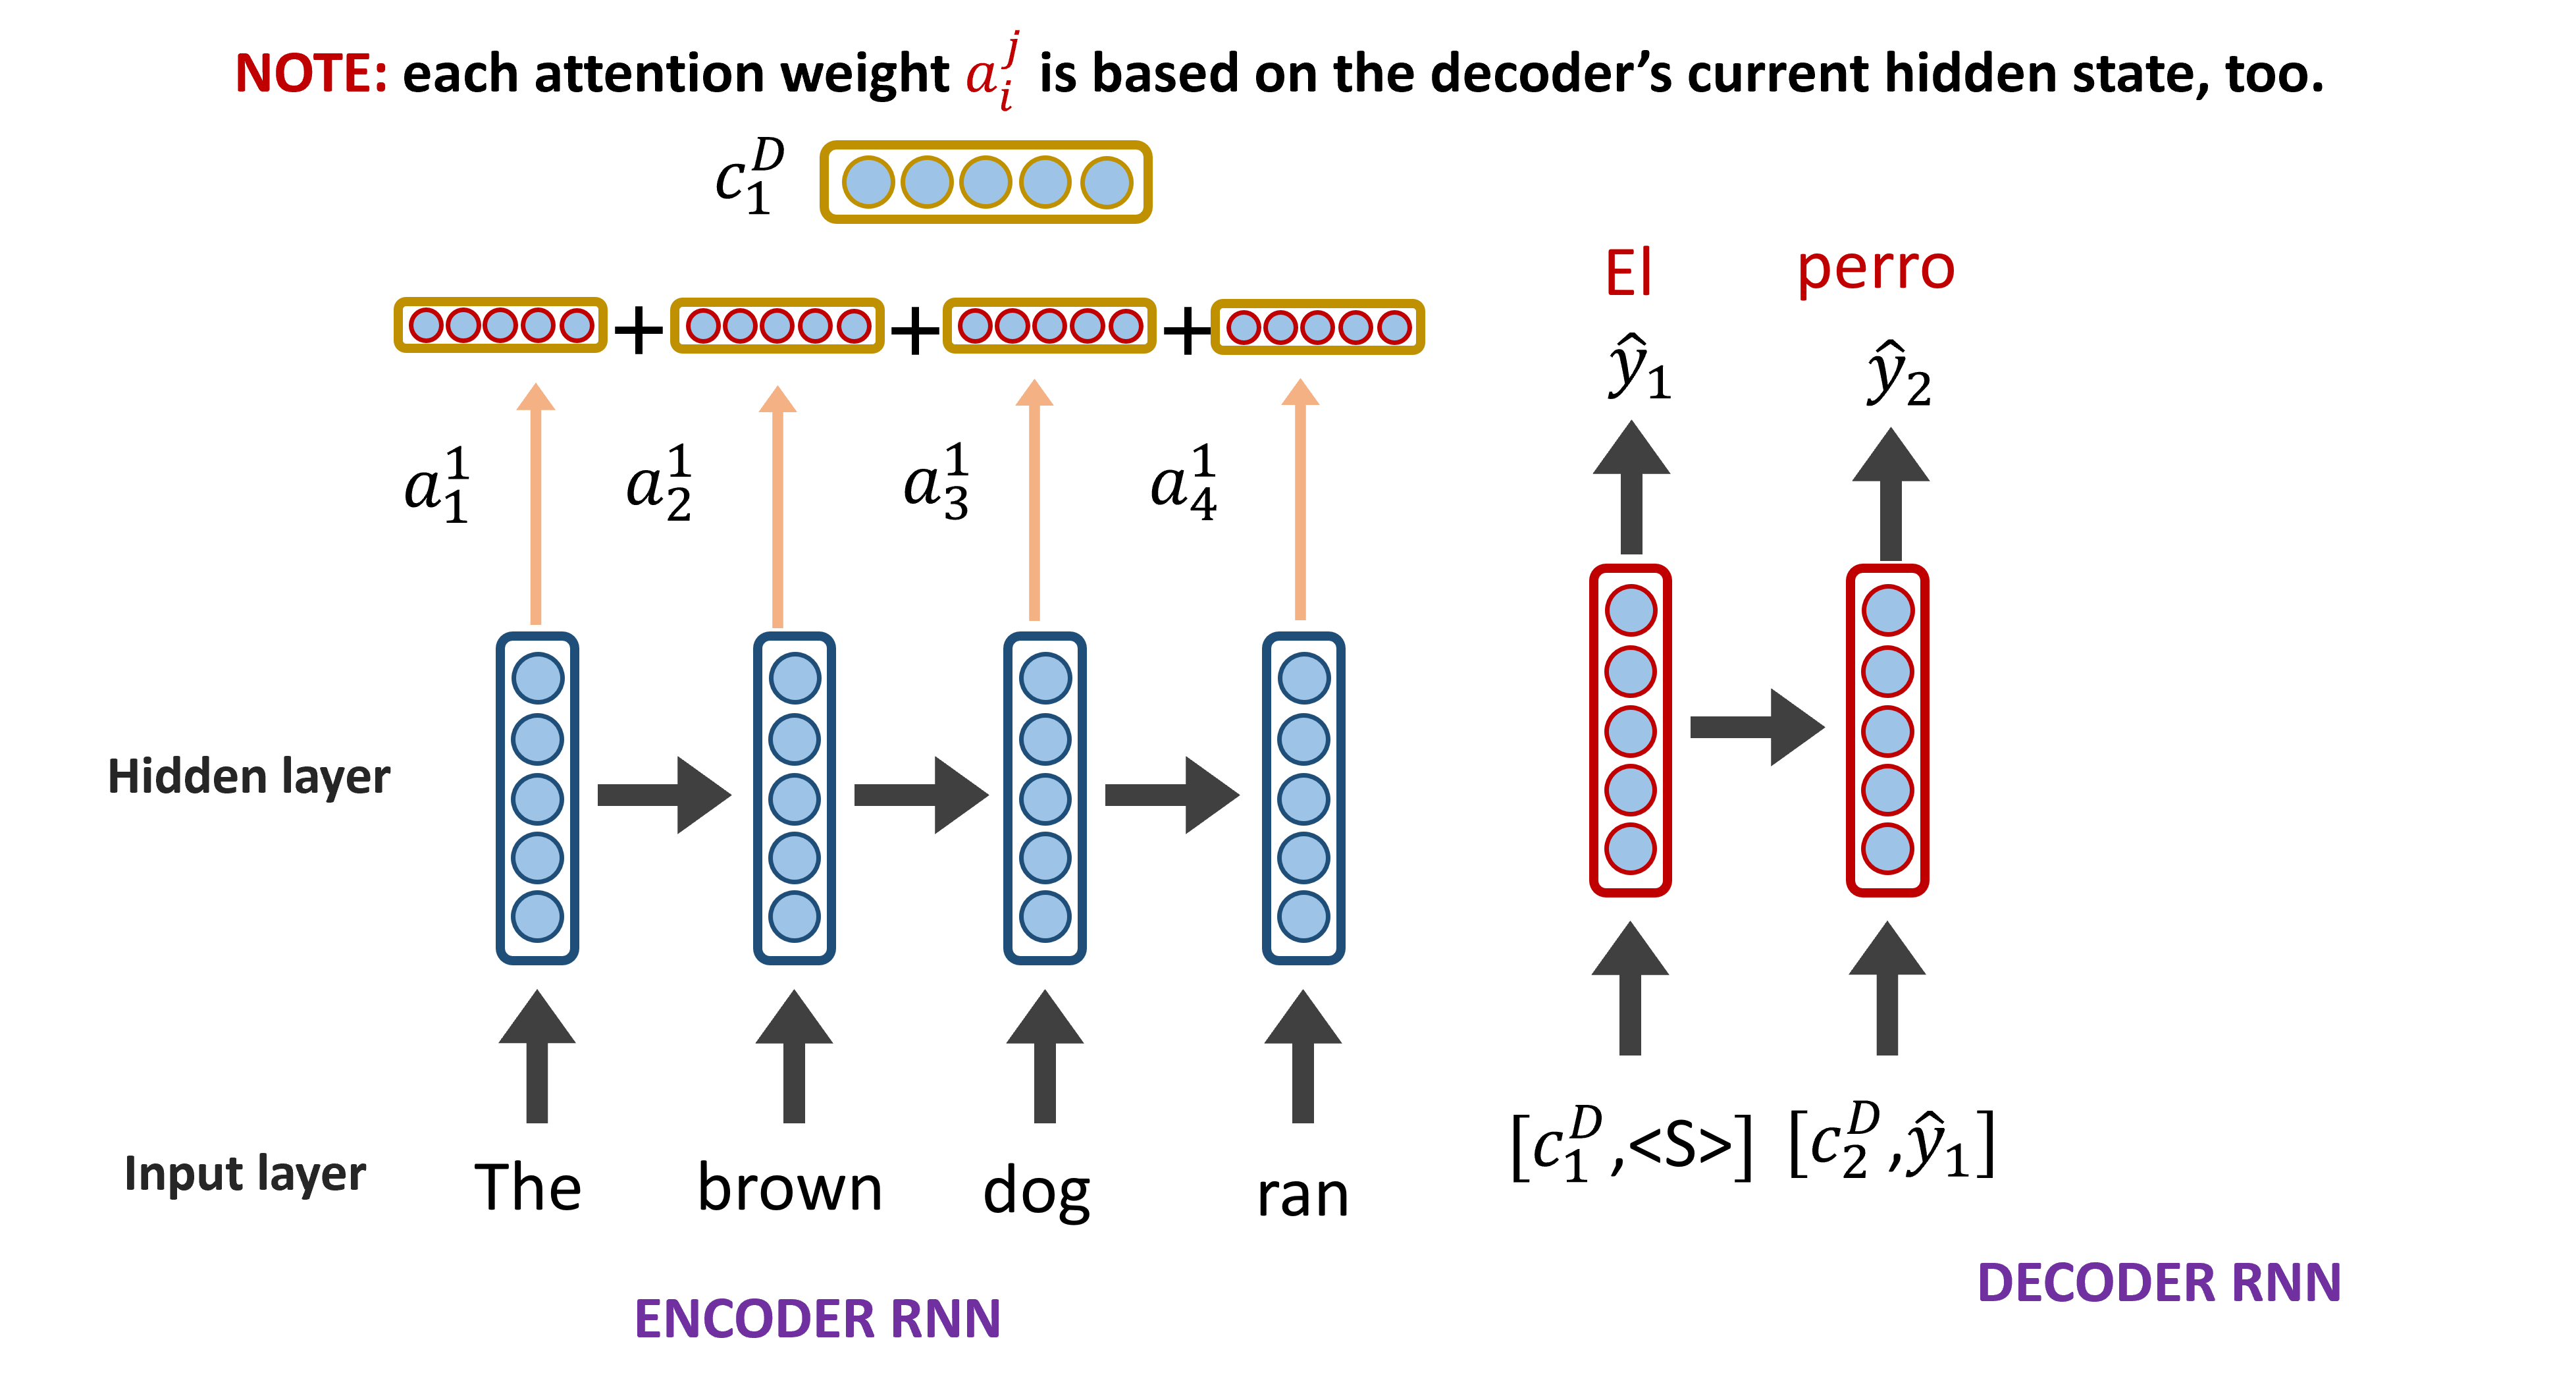
\includegraphics[width=0.8\linewidth,keepaspectratio]{bert27}
\end{center}	

\end{frame}


%%%%%%%%%%%%%%%%%%%%%%%%%%%%%%%%%%%%%%%%%%%%%%%%%%%%%%%%%%%
\begin{frame}[fragile]\frametitle{seq2seq + Attention}

\begin{center}
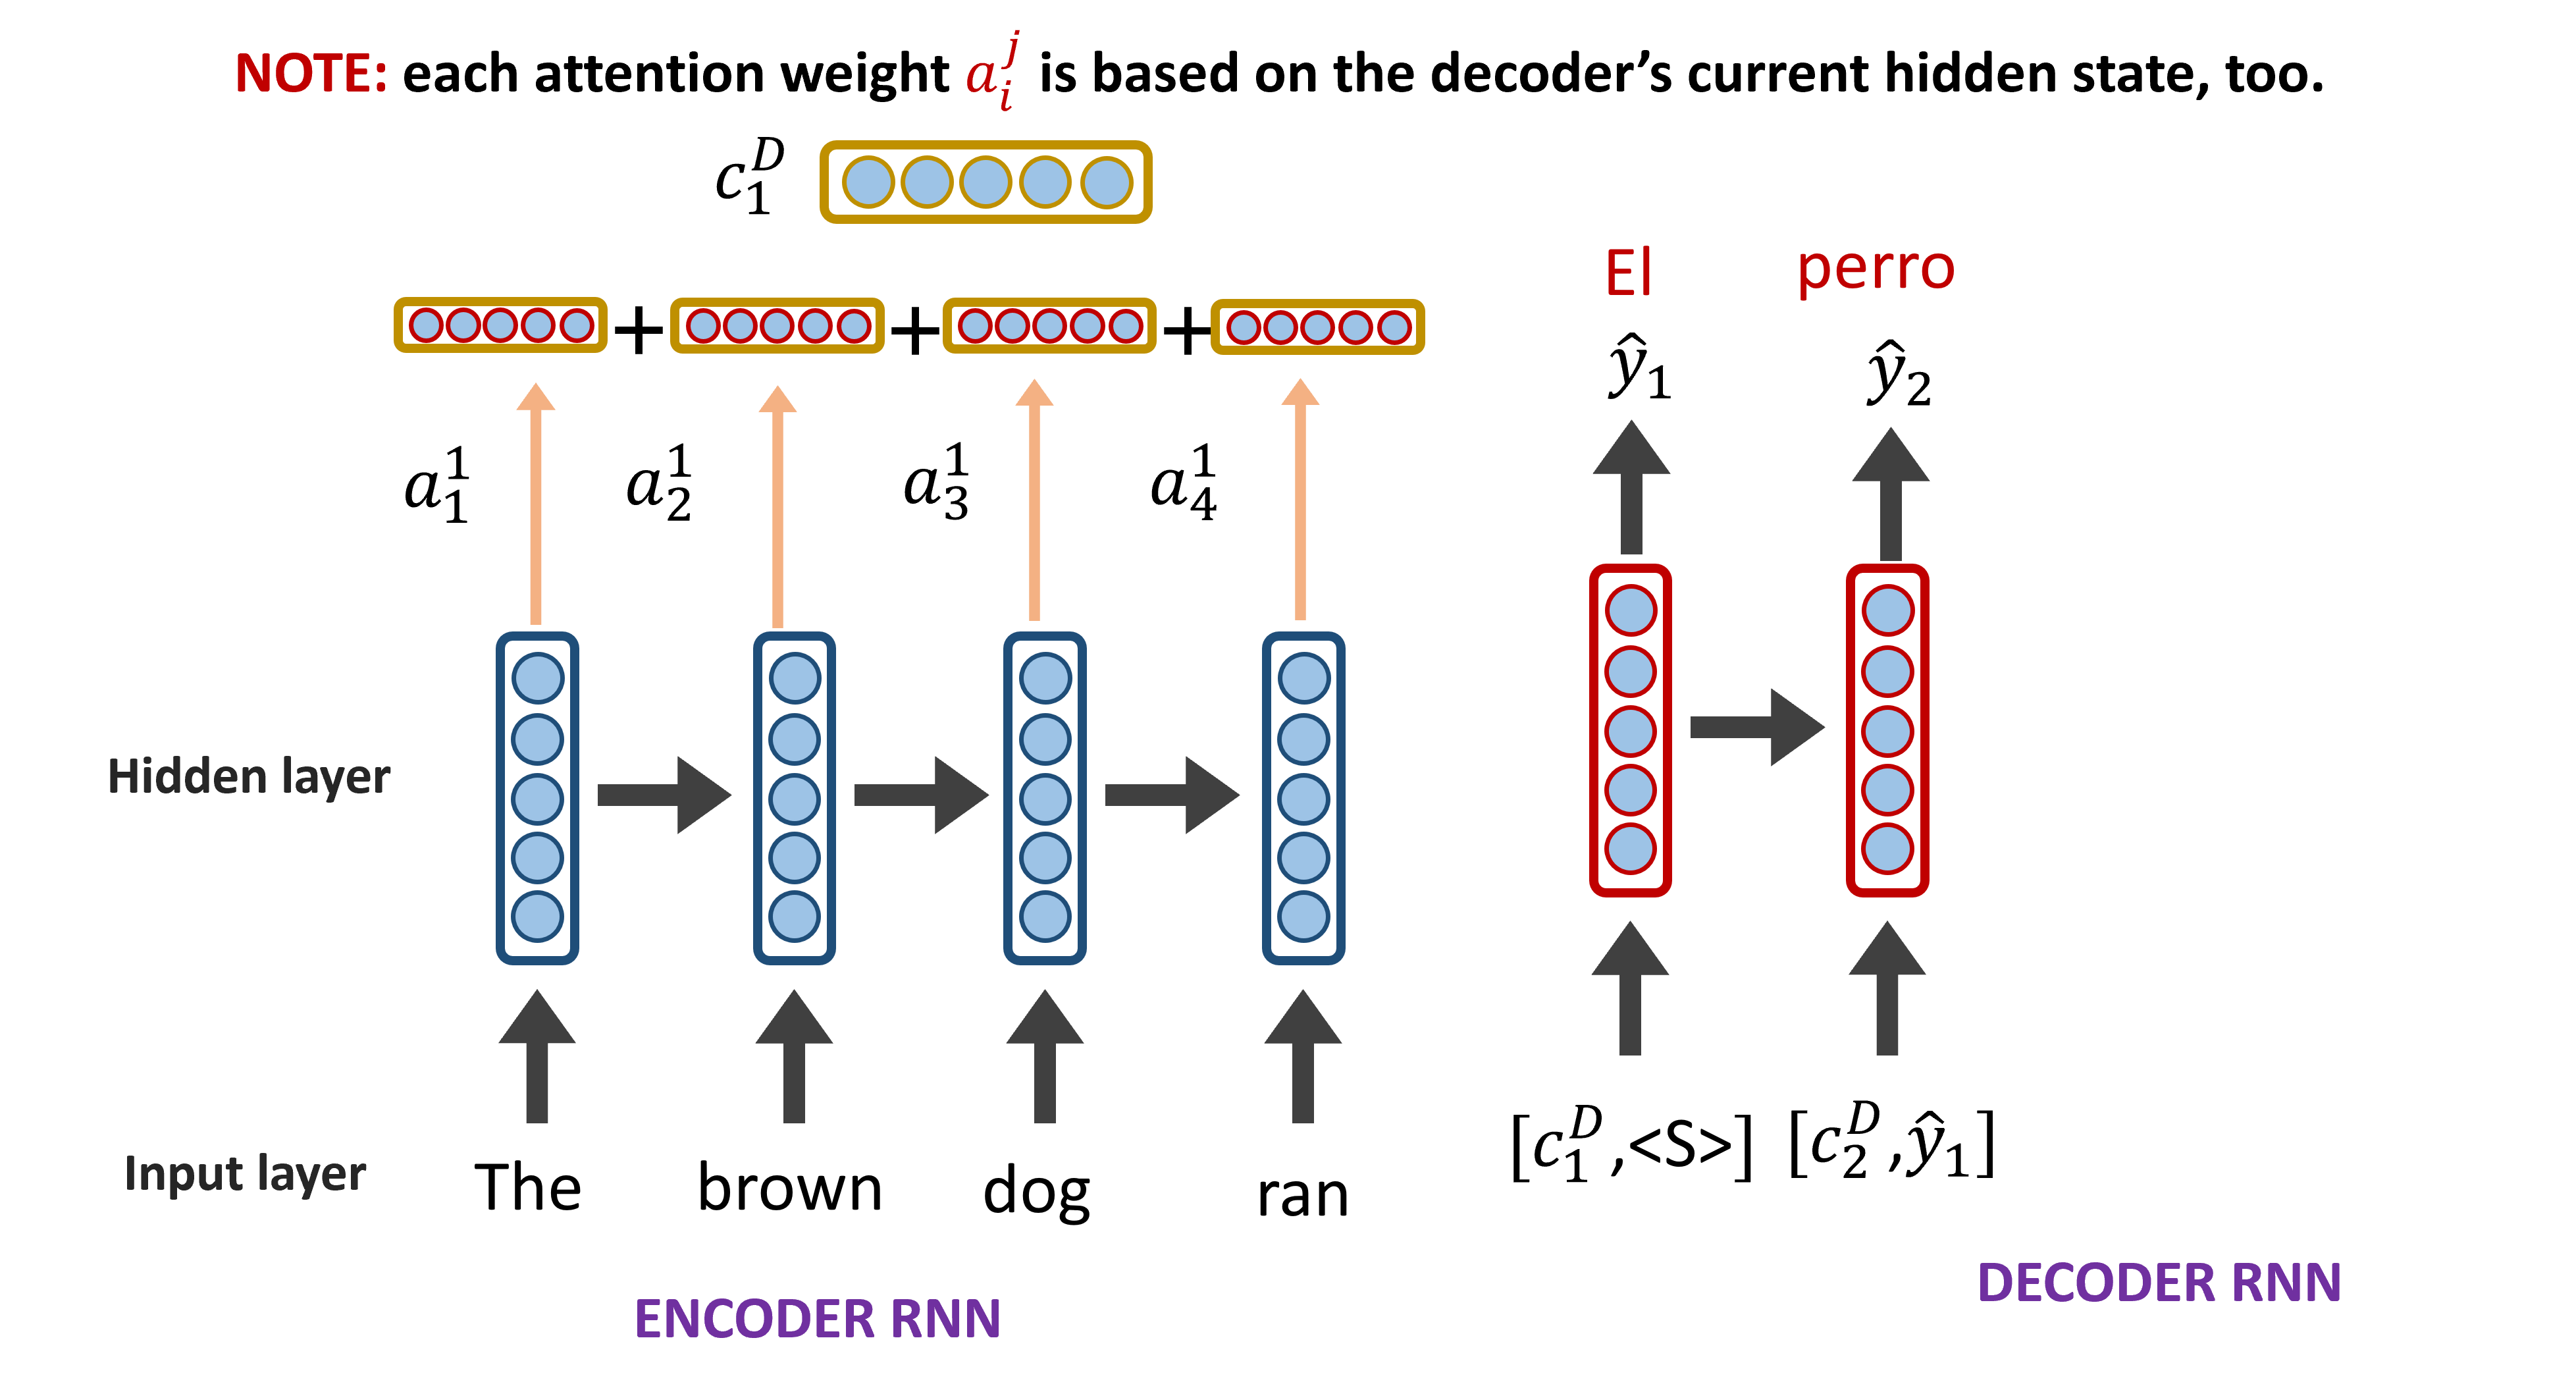
\includegraphics[width=0.8\linewidth,keepaspectratio]{bert28}
\end{center}	

\end{frame}

%%%%%%%%%%%%%%%%%%%%%%%%%%%%%%%%%%%%%%%%%%%%%%%%%%%%%%%%%%%
\begin{frame}[fragile]\frametitle{seq2seq + Attention}

\begin{center}
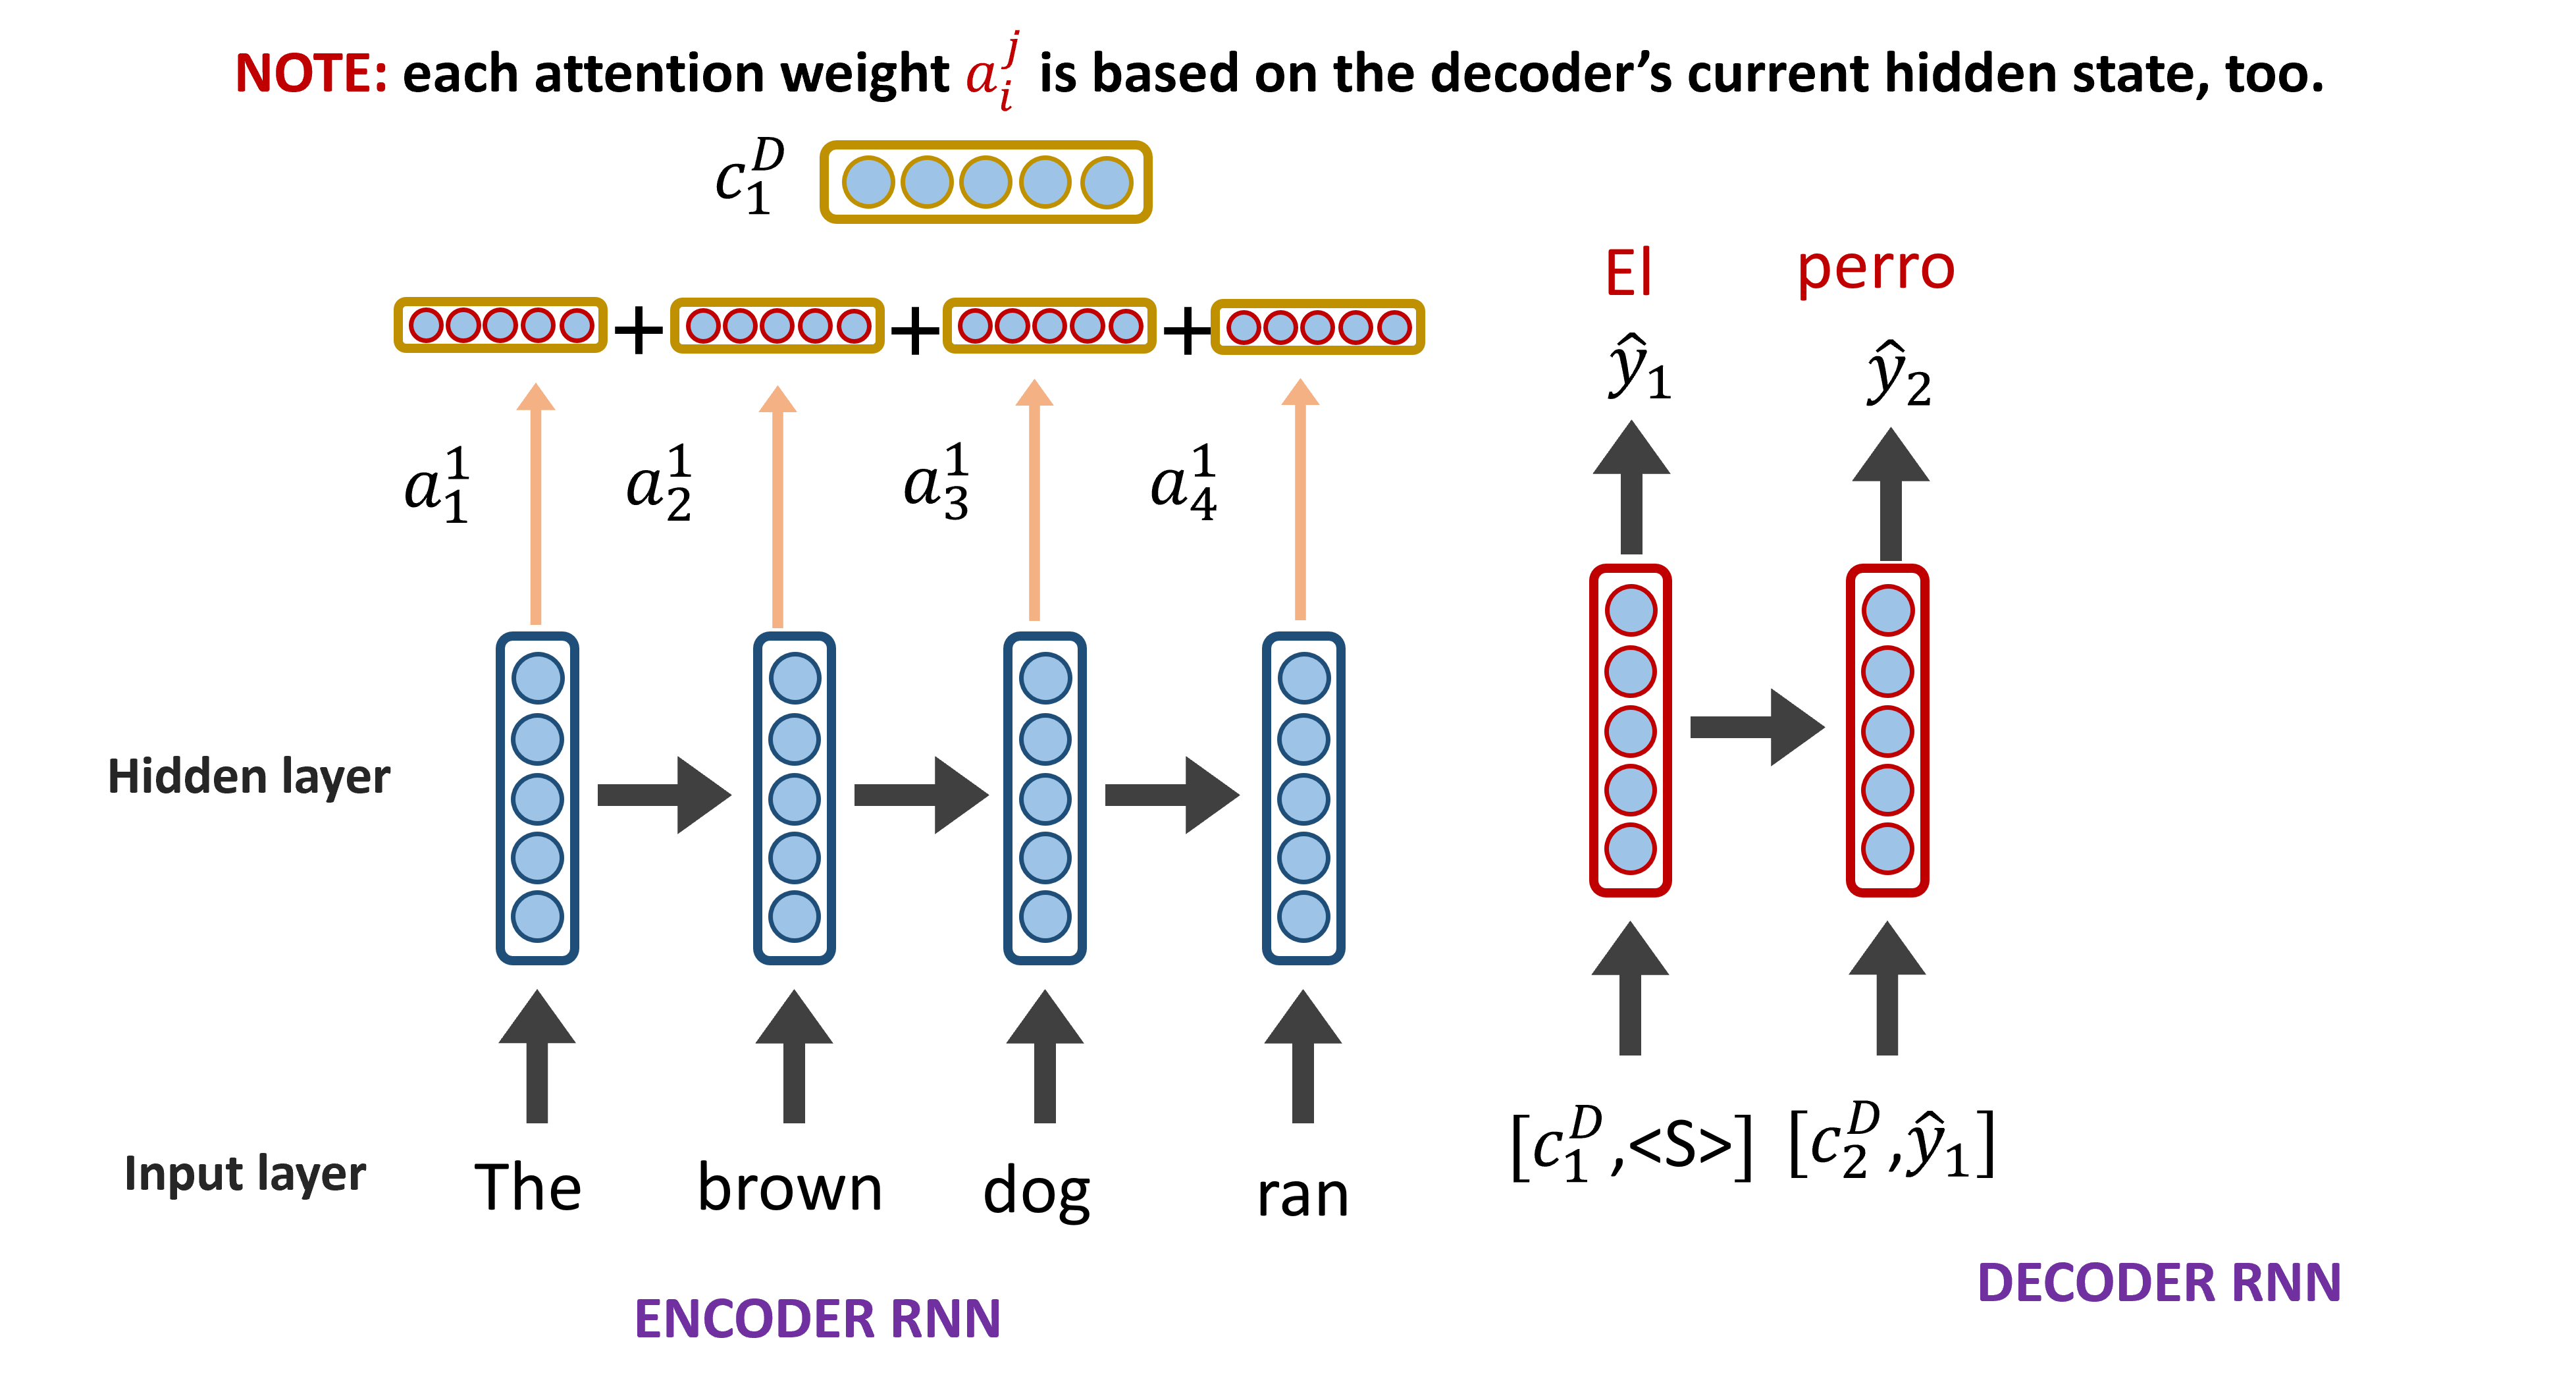
\includegraphics[width=0.8\linewidth,keepaspectratio]{bert29}
\end{center}	

\end{frame}

%%%%%%%%%%%%%%%%%%%%%%%%%%%%%%%%%%%%%%%%%%%%%%%%%%%%%%%%%%%
\begin{frame}[fragile]\frametitle{seq2seq + Attention}

\begin{center}
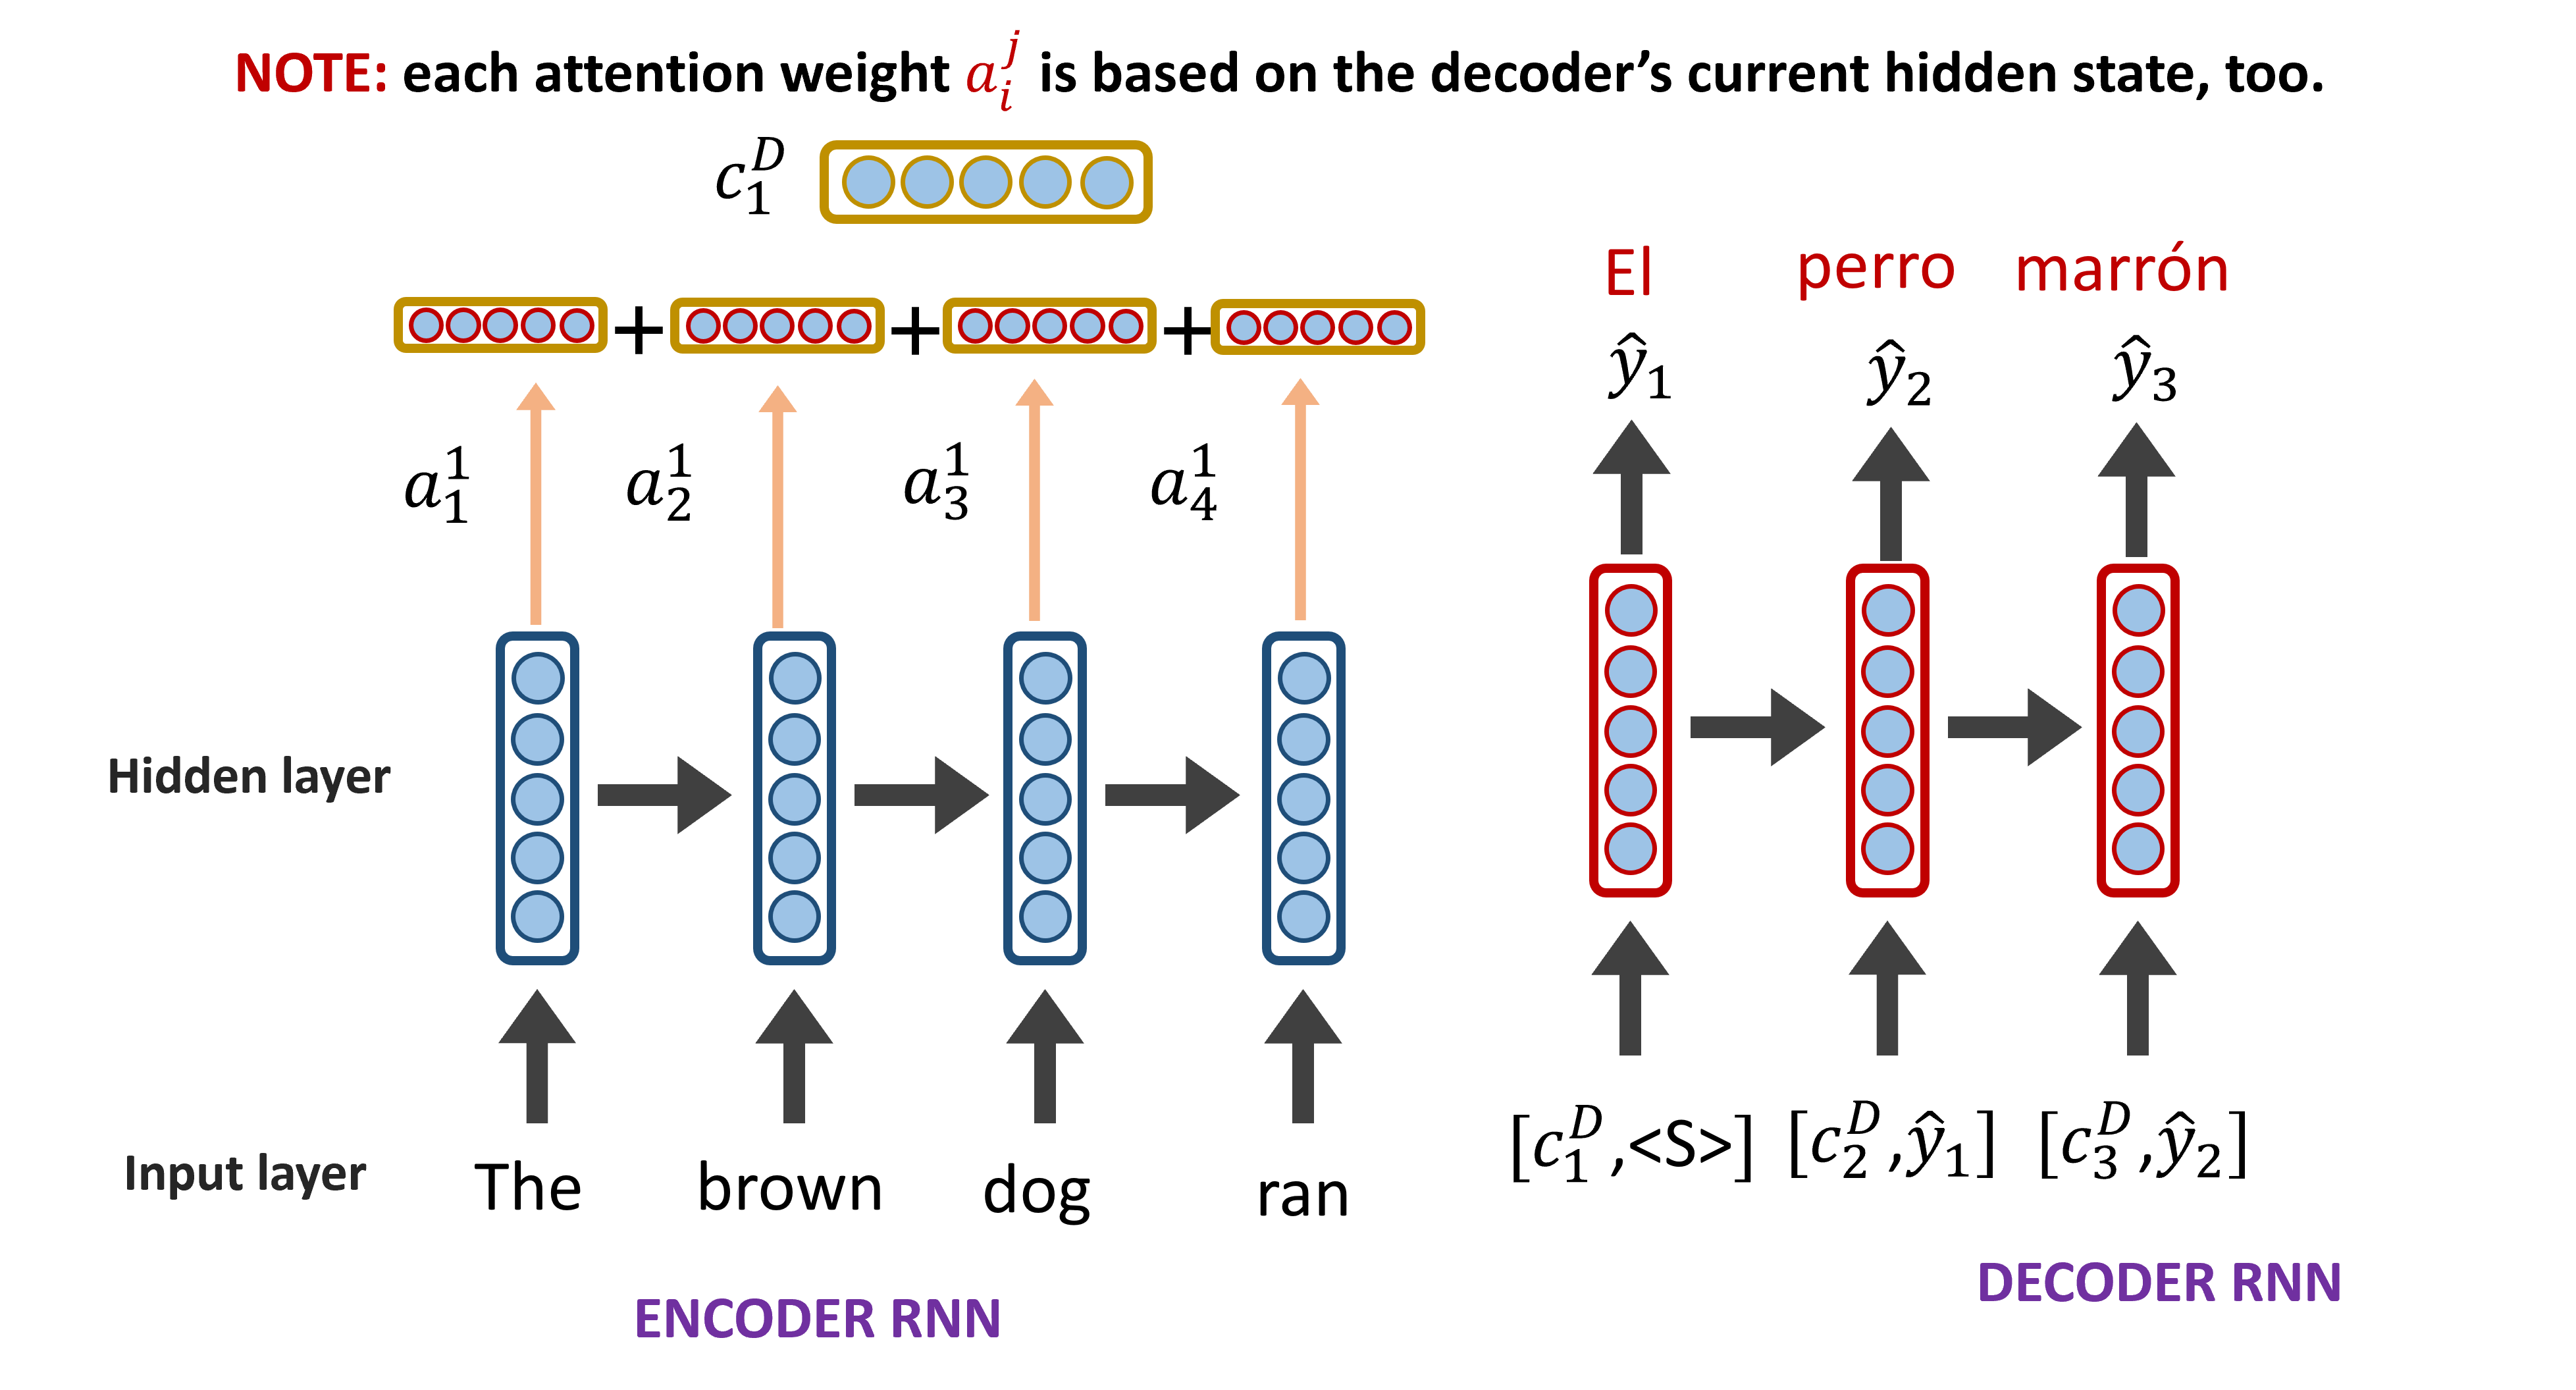
\includegraphics[width=0.8\linewidth,keepaspectratio]{bert30}
\end{center}	

\end{frame}

%%%%%%%%%%%%%%%%%%%%%%%%%%%%%%%%%%%%%%%%%%%%%%%%%%%%%%%%%%%
\begin{frame}[fragile]\frametitle{seq2seq + Attention}

\begin{center}
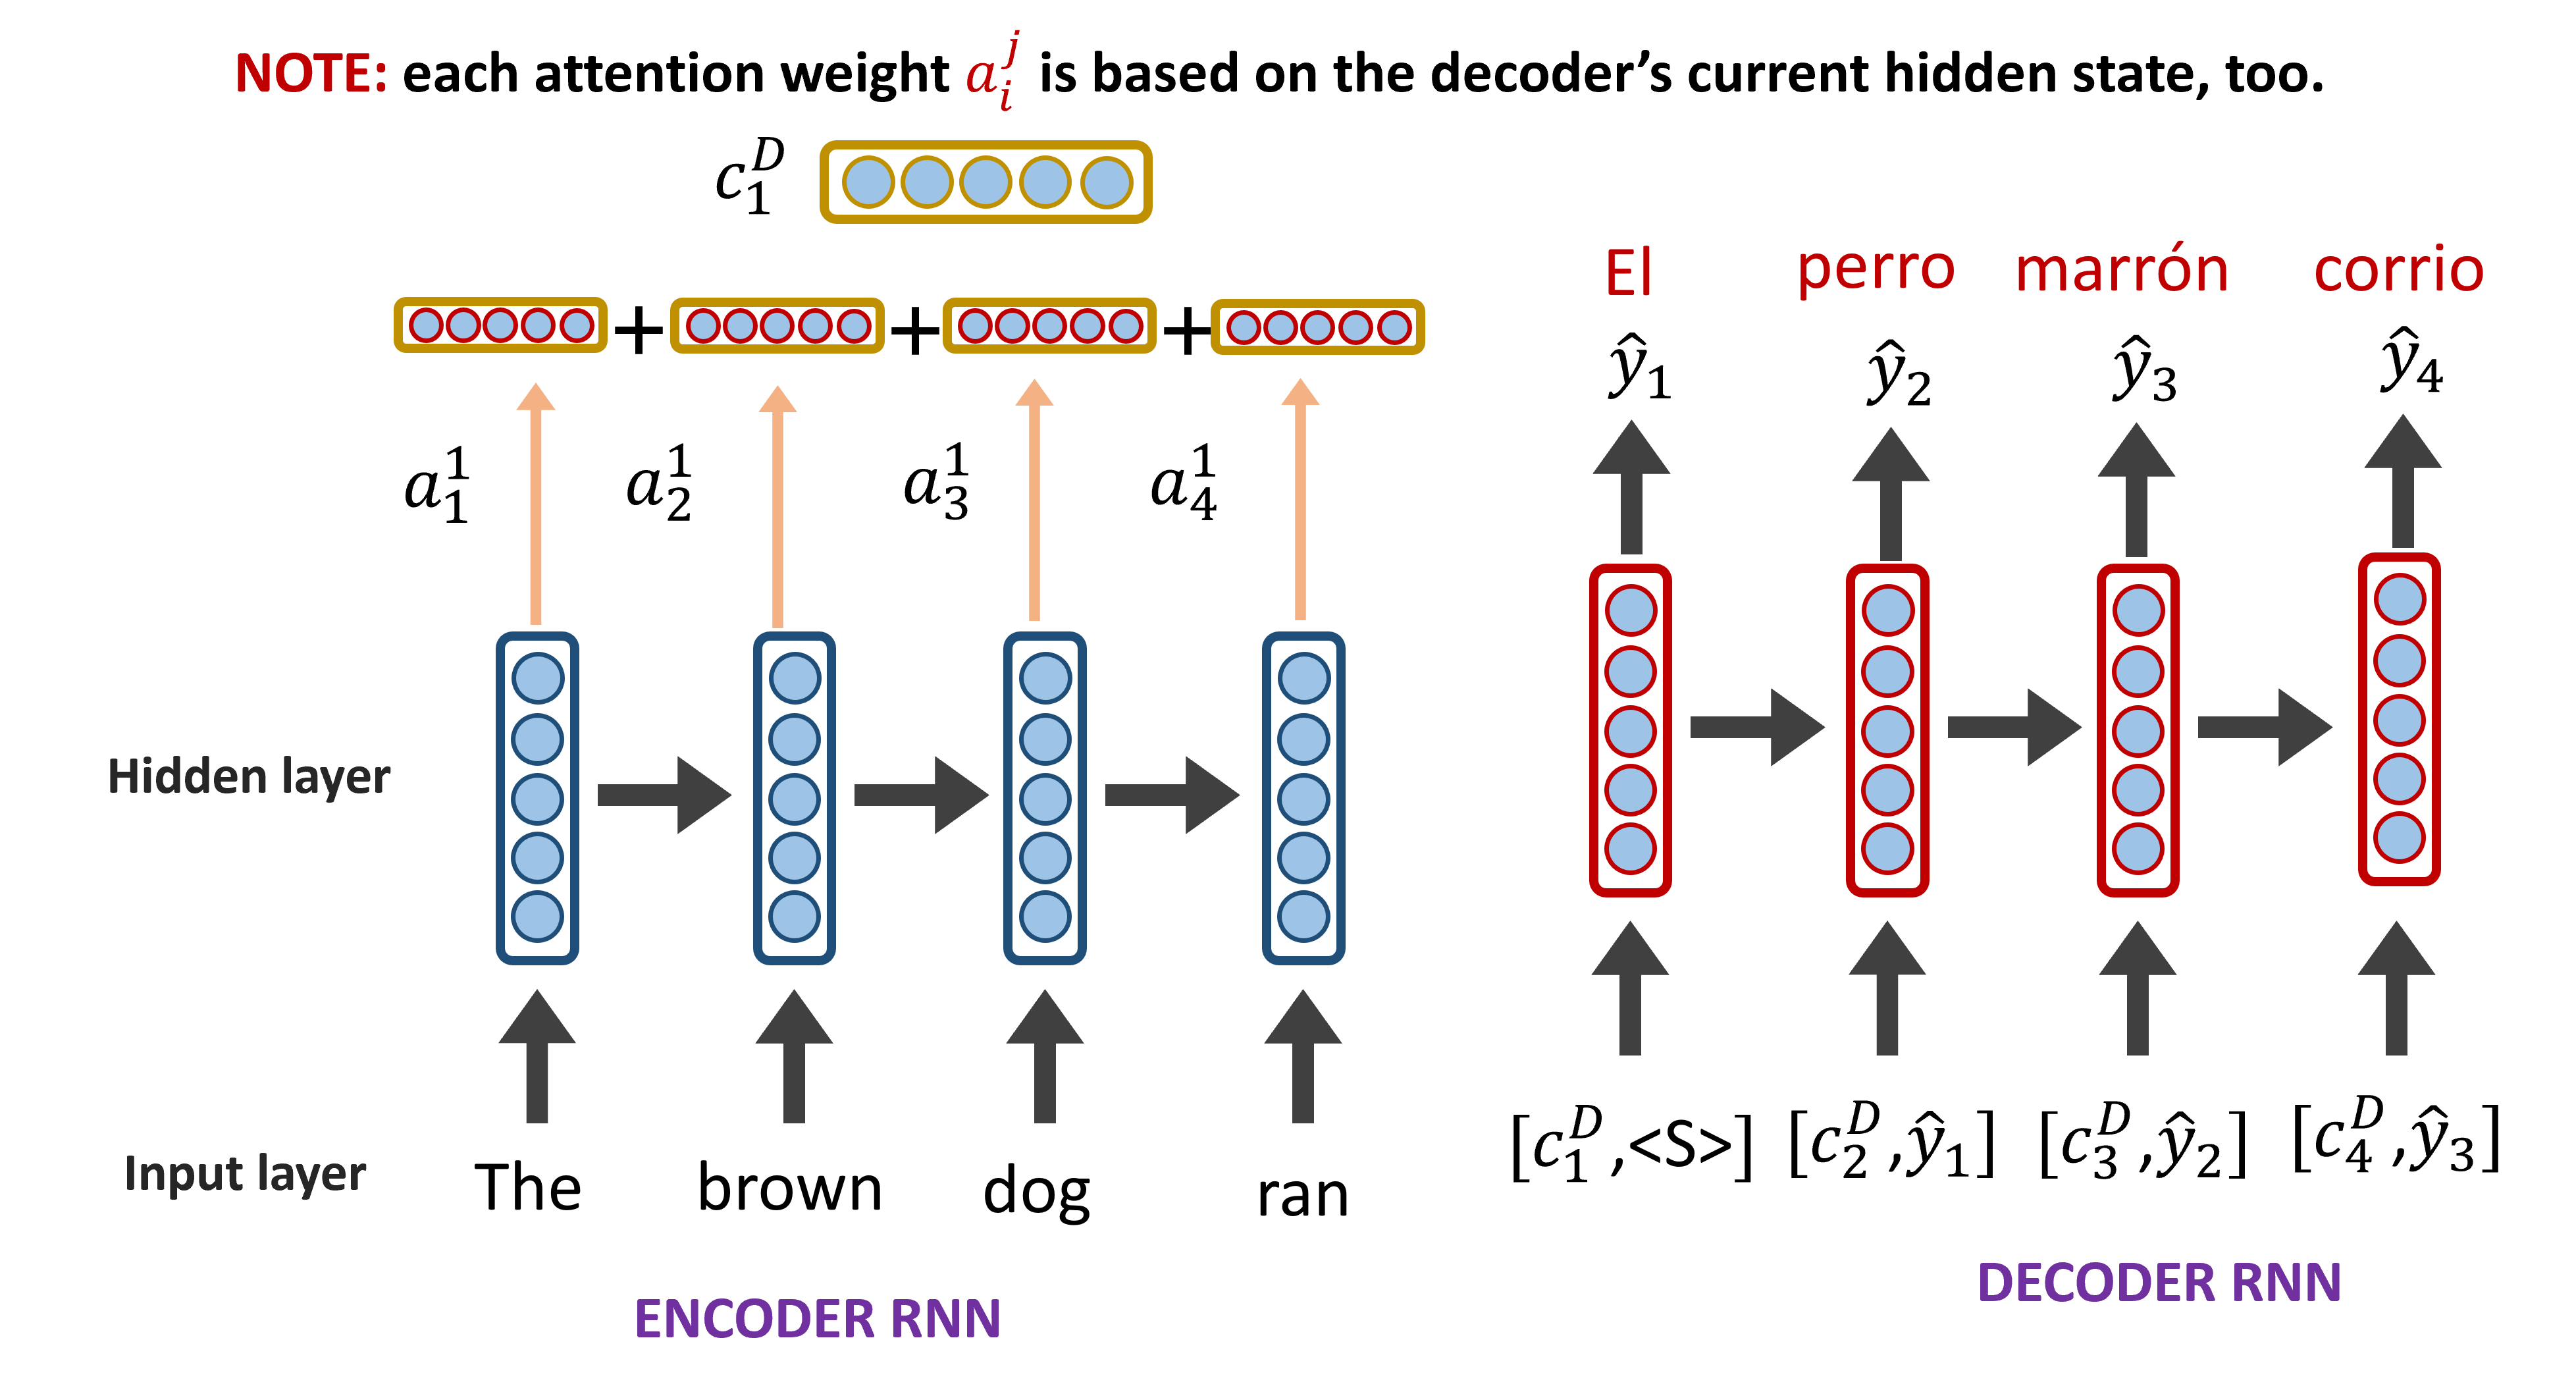
\includegraphics[width=0.8\linewidth,keepaspectratio]{bert31}
\end{center}	

\end{frame}

%%%%%%%%%%%%%%%%%%%%%%%%%%%%%%%%%%%%%%%%%%%%%%%%%%%%%%%%%%%
\begin{frame}[fragile]\frametitle{seq2seq + Attention}

\begin{center}
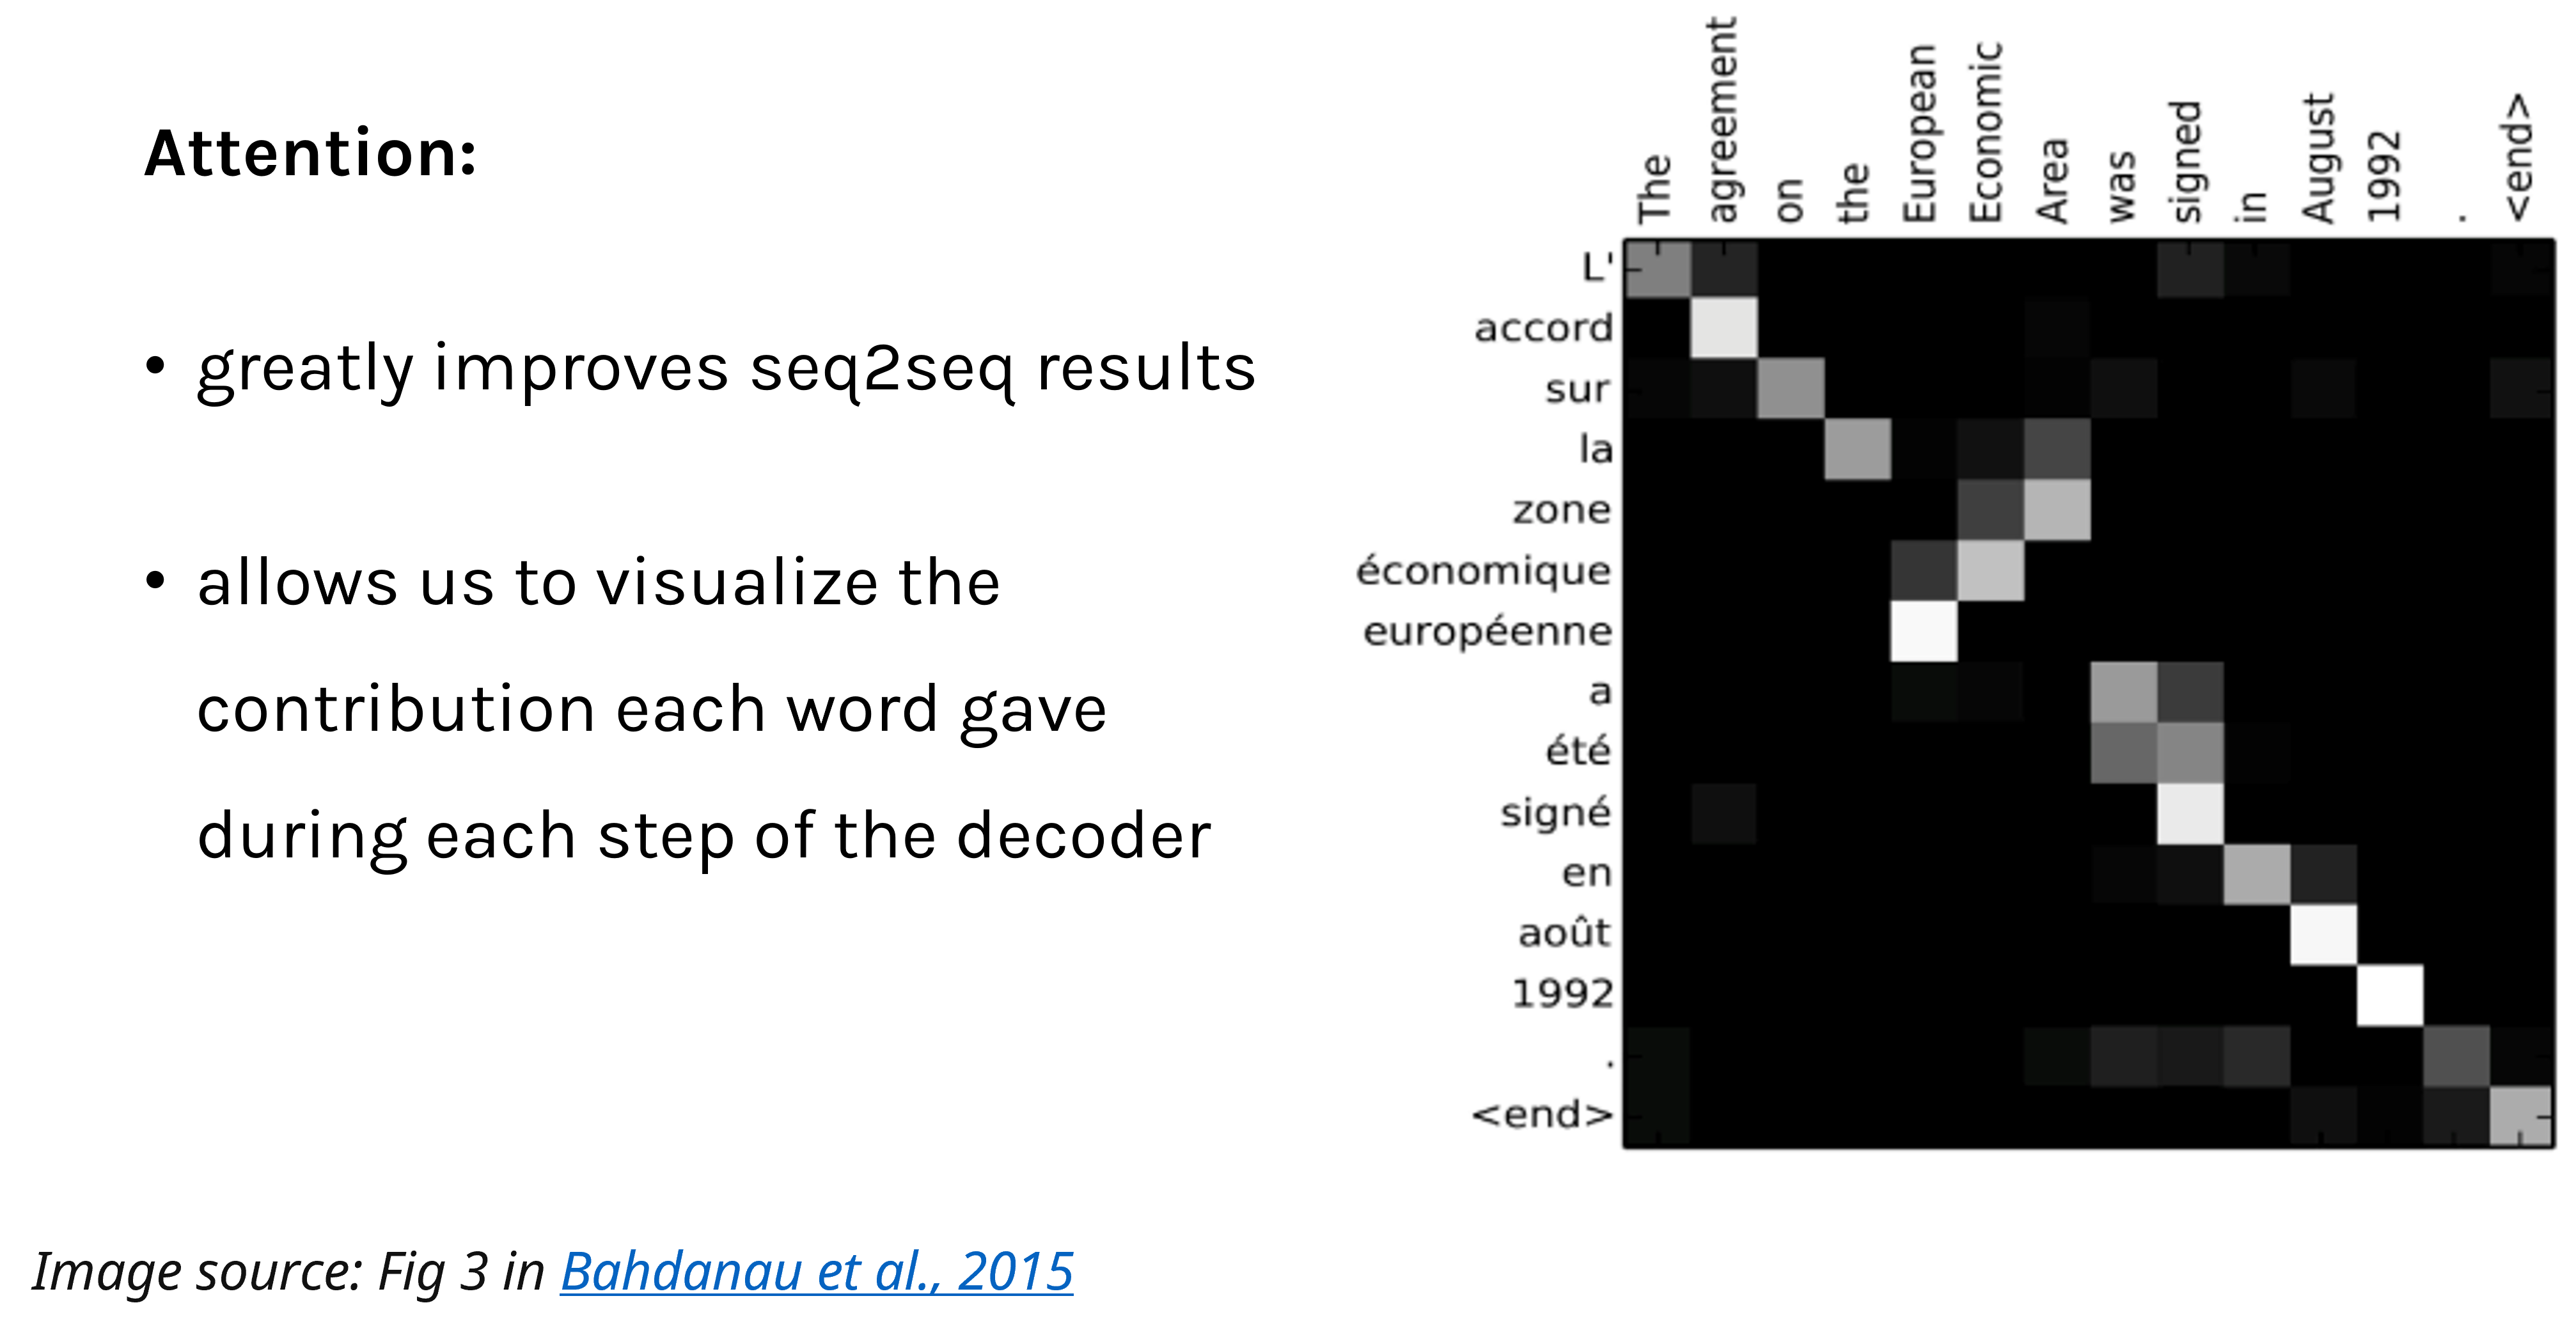
\includegraphics[width=\linewidth,keepaspectratio]{bert32}
\end{center}	

\end{frame}

%%%%%%%%%%%%%%%%%%%%%%%%%%%%%%%%%%%%%%%%%%%%%%%%%%%%%%%%%%%%%%%%%%%%%%%%%%%%%%%%%%
\begin{frame}[fragile]\frametitle{}
\begin{center}
{\Large Embeddings}
\end{center}
\end{frame}

%%%%%%%%%%%%%%%%%%%%%%%%%%%%%%%%%%%%%%%%%%%%%%%%%%%%%%%%%%%
\begin{frame}[fragile]\frametitle{ELMo: Embeddings from Language  Models}

Deep contextualized word representations. Peters et al. NAACL 2018.  https://arxiv.org/abs/1802.05365

\begin{itemize}
\item ``Instead of using a fixed embedding for each word, ELMo looks at the entire sentence before assigning each word in it an embedding.''
\item Breakout version of word token vectors or
contextual word vectors
\item Learn word token vectors using long contexts not context  windows (here, whole sentence, could be longer)
\item Learn a deep Bi-NLM and use all its layers in prediction
\end{itemize}

{\tiny (Ref: CS224n: Natural Language Processing with Deep Learning - Christopher Manning)}

\end{frame}

%%%%%%%%%%%%%%%%%%%%%%%%%%%%%%%%%%%%%%%%%%%%%%%%%%%%%%%%%%%
\begin{frame}[fragile]\frametitle{ELMo: Embeddings from Language  Models}

\begin{itemize}
\item Train a bidirectional LM
\item Aim at performant but not overly large LM:

\begin{itemize}
\item Use 2 biLSTM layers
\item Use character CNN to build initial word representation 
\item User 4096 dim hidden/cell LSTM states with 512 dim projections to next input
\item Use a residual connection
\item Tie parameters of token input and output (softmax) and tie these between forward and backward LMs
\end{itemize}

\end{itemize}

{\tiny (Ref: CS224n: Natural Language Processing with Deep Learning - Christopher Manning)}

\end{frame}

%%%%%%%%%%%%%%%%%%%%%%%%%%%%%%%%%%%%%%%%%%%%%%%%%%%%%%%%%%%
\begin{frame}[fragile]\frametitle{ELMo used in a sequence tagger}

\begin{center}
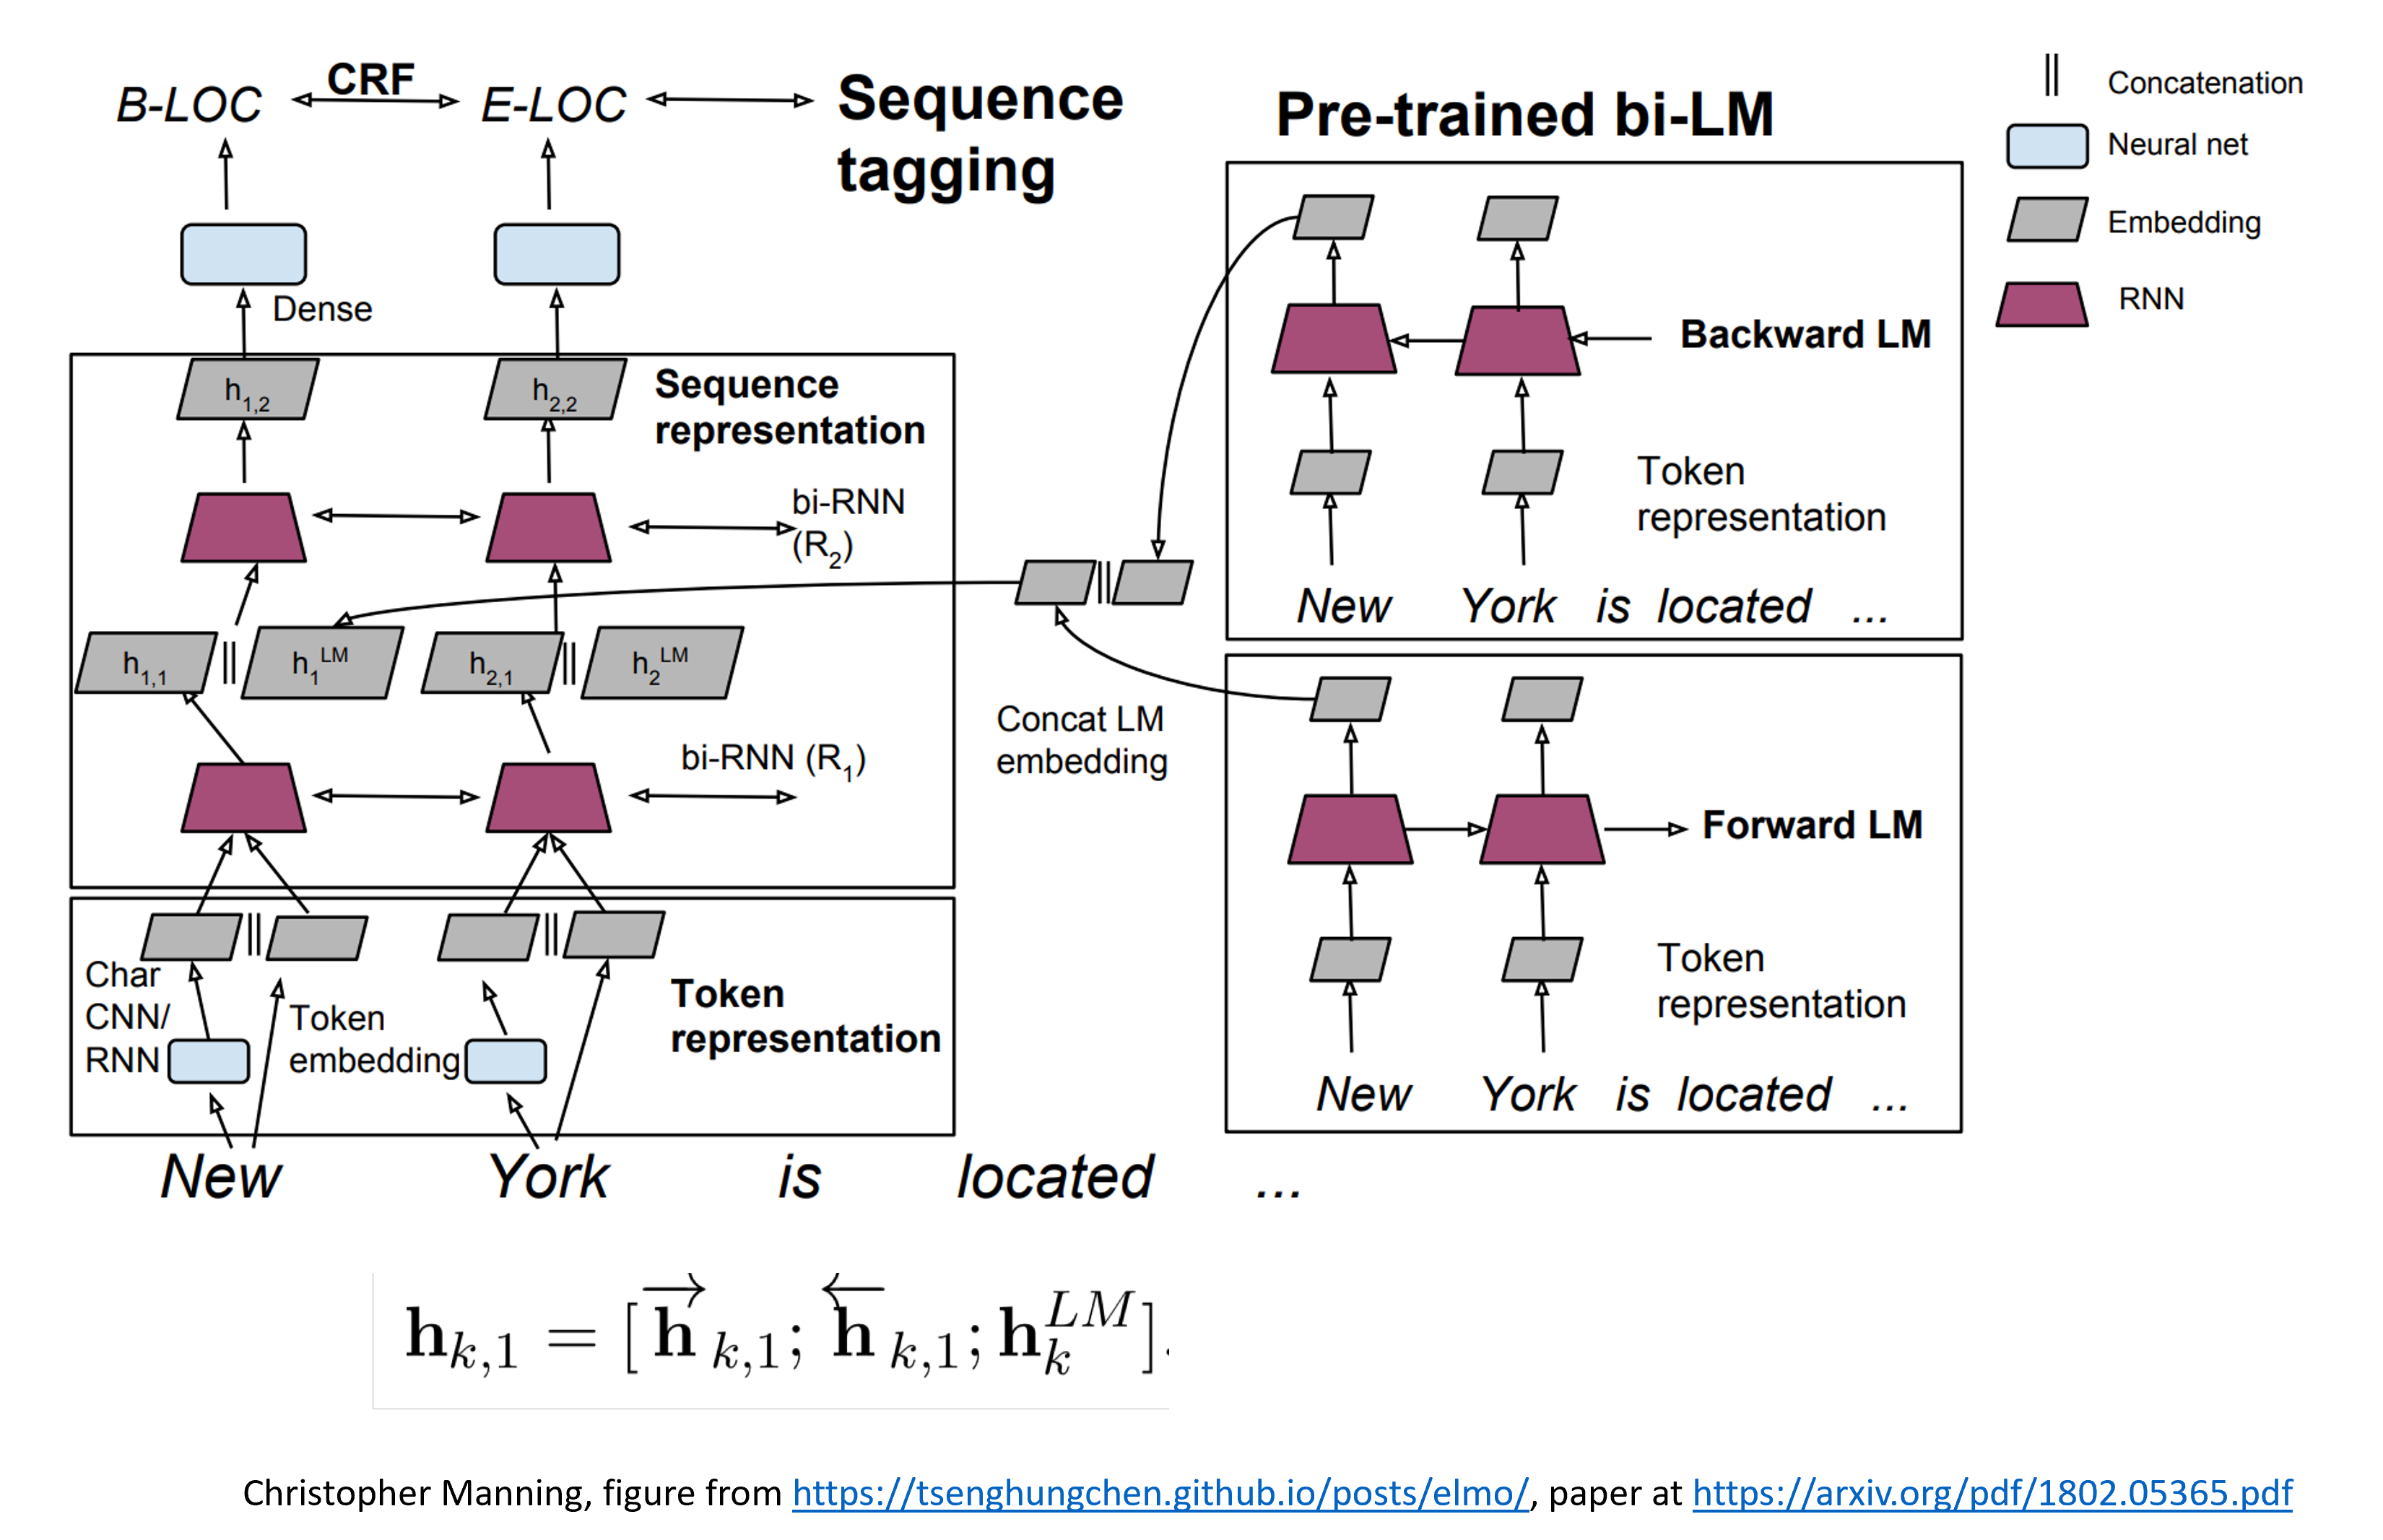
\includegraphics[width=\linewidth,keepaspectratio]{bert33}
\end{center}	

{\tiny (Ref: CS224n: Natural Language Processing with Deep Learning - Christopher Manning)}

\end{frame}

%%%%%%%%%%%%%%%%%%%%%%%%%%%%%%%%%%%%%%%%%%%%%%%%%%%%%%%%%%%
\begin{frame}[fragile]\frametitle{ELMo results: Great for all tasks}

\begin{center}
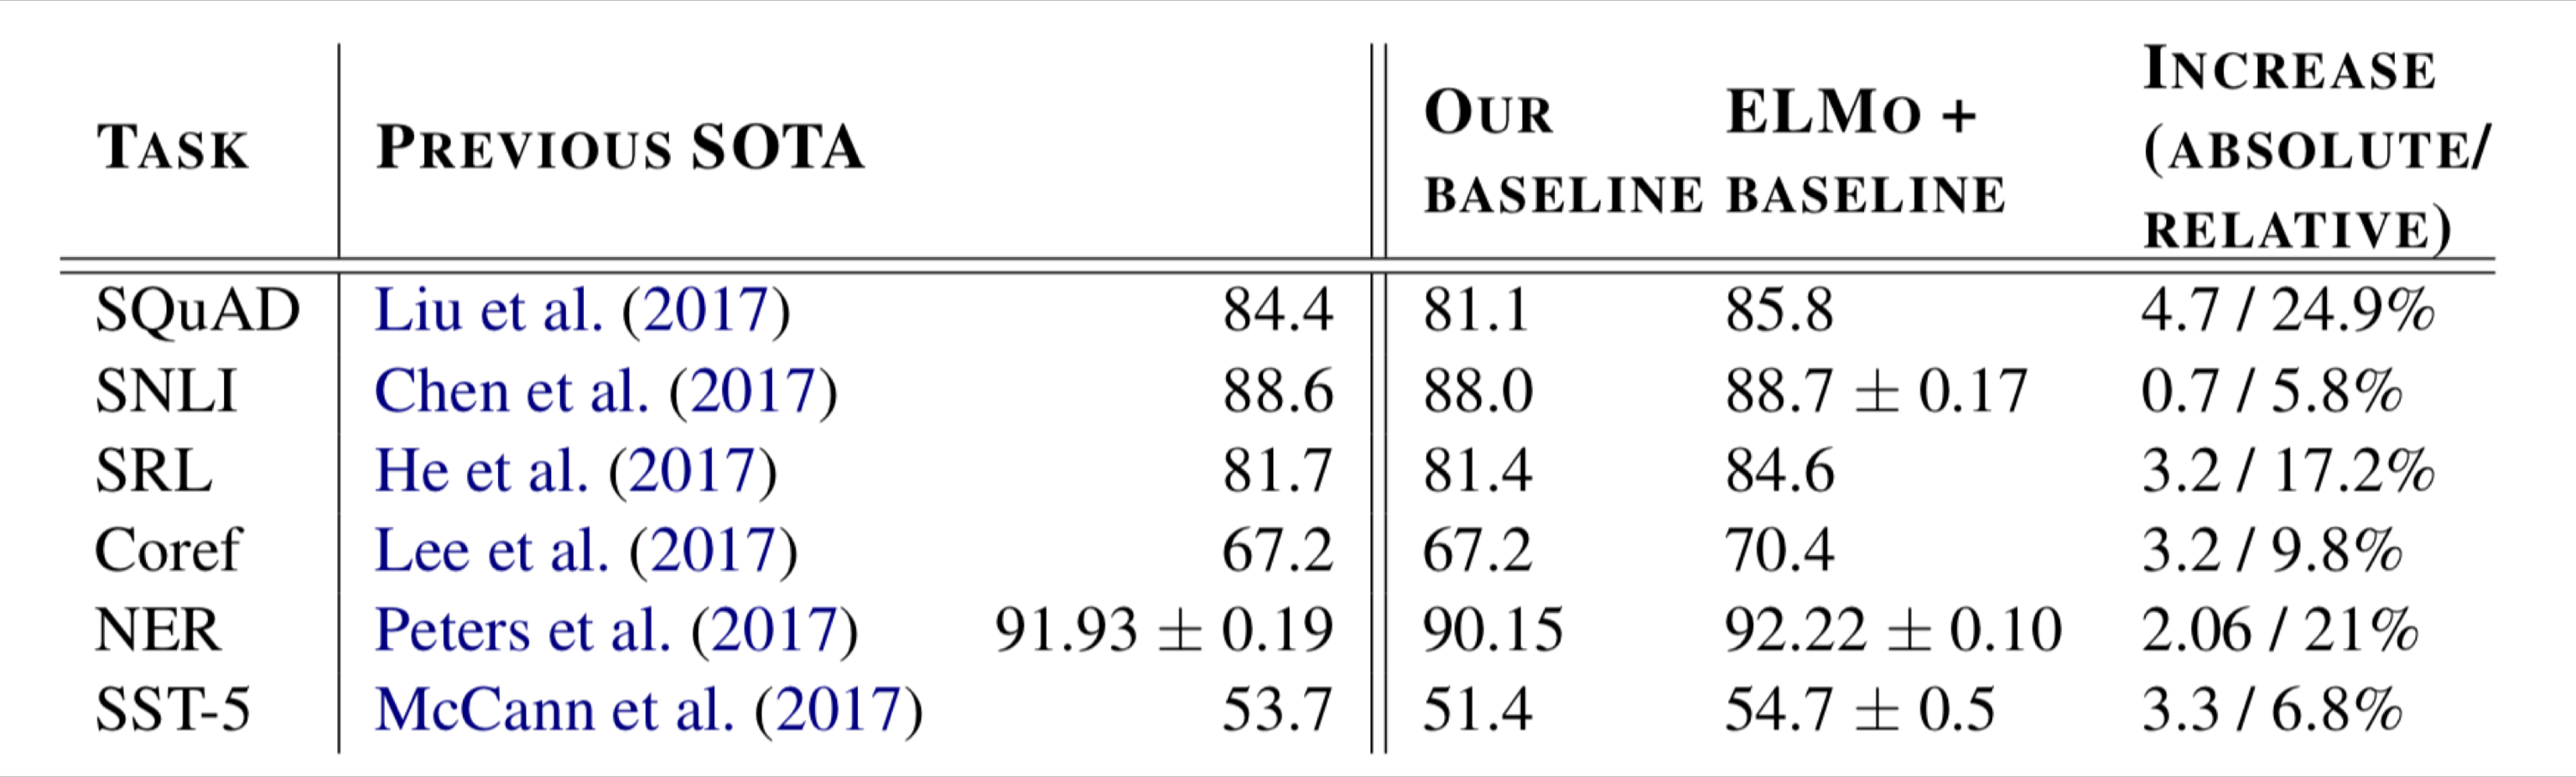
\includegraphics[width=\linewidth,keepaspectratio]{bert34}
\end{center}	

{\tiny (Ref: CS224n: Natural Language Processing with Deep Learning - Christopher Manning)}

\end{frame}

%%%%%%%%%%%%%%%%%%%%%%%%%%%%%%%%%%%%%%%%%%%%%%%%%%%%%%%%%%%
\begin{frame}[fragile]\frametitle{ELMo: Roles of different layers}

The two biLSTM NLM layers have differentiated uses/meanings

\begin{itemize}
\item Lower layer is better for lower-level syntax, etc.
Part-of-speech tagging, syntactic dependencies, NER
\item Higher layer is better for higher-level semantics
Sentiment, Semantic role labeling, question answering, SNLI

\end{itemize}


{\tiny (Ref: CS224n: Natural Language Processing with Deep Learning - Christopher Manning)}

\end{frame}

%%%%%%%%%%%%%%%%%%%%%%%%%%%%%%%%%%%%%%%%%%%%%%%%%%%%%%%%%%%
\begin{frame}[fragile]\frametitle{Issues with recurrent models: Linear interaction distance}

O(sequence length) steps for distant word pairs to interact means:

\begin{itemize}
\item Hard to learn long-distance dependencies (because gradient problems!)
\item Linear order of words is ``baked in''; not necessarily the  right way to think about sentences \ldots
\end{itemize}	 

\begin{center}
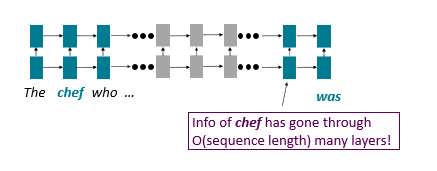
\includegraphics[width=\linewidth,keepaspectratio]{bert35}
\end{center}	

 
{\tiny (Ref: Language \& Machine Learning - John Hewitt)}
\end{frame}

%%%%%%%%%%%%%%%%%%%%%%%%%%%%%%%%%%%%%%%%%%%%%%%%%%%%%%%%%%%
\begin{frame}[fragile]\frametitle{Issues with recurrent models: Lack of parallelizability}

Forward and backward passes have O(sequence length) unparallelizable operations

\begin{itemize}
\item GPUs can perform a bunch of independent computations at once!
\item But future RNN hidden states can’t be computed in full before past RNN
hidden states have been computed
\item Inhibits training on very large datasets!
\end{itemize}	 

\begin{center}
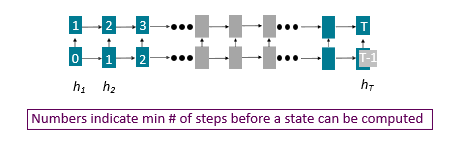
\includegraphics[width=\linewidth,keepaspectratio]{bert36}
\end{center}	

 
{\tiny (Ref: Language \& Machine Learning - John Hewitt)}
\end{frame}

%%%%%%%%%%%%%%%%%%%%%%%%%%%%%%%%%%%%%%%%%%%%%%%%%%%%%%%%%%%
\begin{frame}[fragile]\frametitle{If not recurrence, then what? How about word windows?}

Word window models aggregate local contexts

\begin{itemize}
\item Also known as 1D convolution
\item Number of unparallelizable operations not tied to sequence length!
\end{itemize}	 

\begin{center}
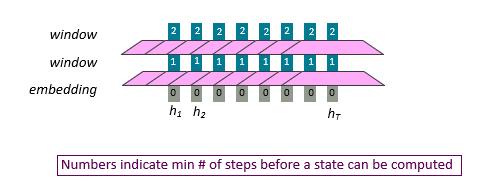
\includegraphics[width=\linewidth,keepaspectratio]{bert37}
\end{center}	

 
{\tiny (Ref: Language \& Machine Learning - John Hewitt)}
\end{frame}

%%%%%%%%%%%%%%%%%%%%%%%%%%%%%%%%%%%%%%%%%%%%%%%%%%%%%%%%%%%
\begin{frame}[fragile]\frametitle{If not recurrence, then what? How about word windows?}

What about long-distance dependencies?

\begin{itemize}
\item Stacking word window layers allows interaction between farther words
\item But if your sequences are too long, you’ll just ignore long-distance context

\end{itemize}	 

\begin{center}
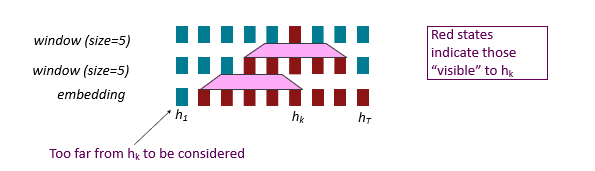
\includegraphics[width=\linewidth,keepaspectratio]{bert38}
\end{center}	

 
{\tiny (Ref: Language \& Machine Learning - John Hewitt)}
\end{frame}

%%%%%%%%%%%%%%%%%%%%%%%%%%%%%%%%%%%%%%%%%%%%%%%%%%%%%%%%%%%
\begin{frame}[fragile]\frametitle{If not recurrence, then what? How about attention?}


\begin{itemize}
\item Attention treats each word’s representation as a query to access and  incorporate information from a set of values.
\item We saw attention from the decoder to the encoder; today we’ll think about
attention within a single sentence.
\item If attention gives us access to any state… maybe we can just use attention and don’t need the RNN?
\item Number of unparallelizable operations not tied to sequence length.
\item All words interact at every layer!

\end{itemize}	 

\begin{center}
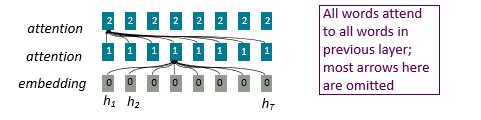
\includegraphics[width=\linewidth,keepaspectratio]{bert39}
\end{center}	

 
{\tiny (Ref: Language \& Machine Learning - John Hewitt)}
\end{frame}

%%%%%%%%%%%%%%%%%%%%%%%%%%%%%%%%%%%%%%%%%%%%%%%%%%%%%%%%%%%
\begin{frame}[fragile]\frametitle{Self-Attention}


\begin{center}
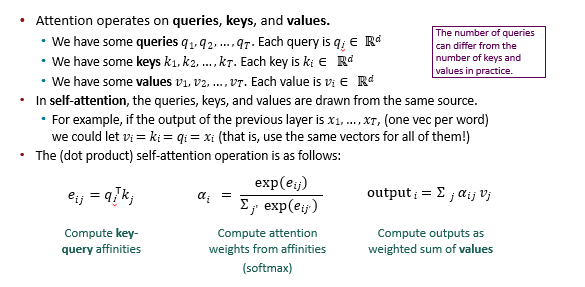
\includegraphics[width=\linewidth,keepaspectratio]{bert40}
\end{center}	

 
{\tiny (Ref: Language \& Machine Learning - John Hewitt)}
\end{frame}

%%%%%%%%%%%%%%%%%%%%%%%%%%%%%%%%%%%%%%%%%%%%%%%%%%%%%%%%%%%
\begin{frame}[fragile]\frametitle{Self-Attention}


\begin{center}
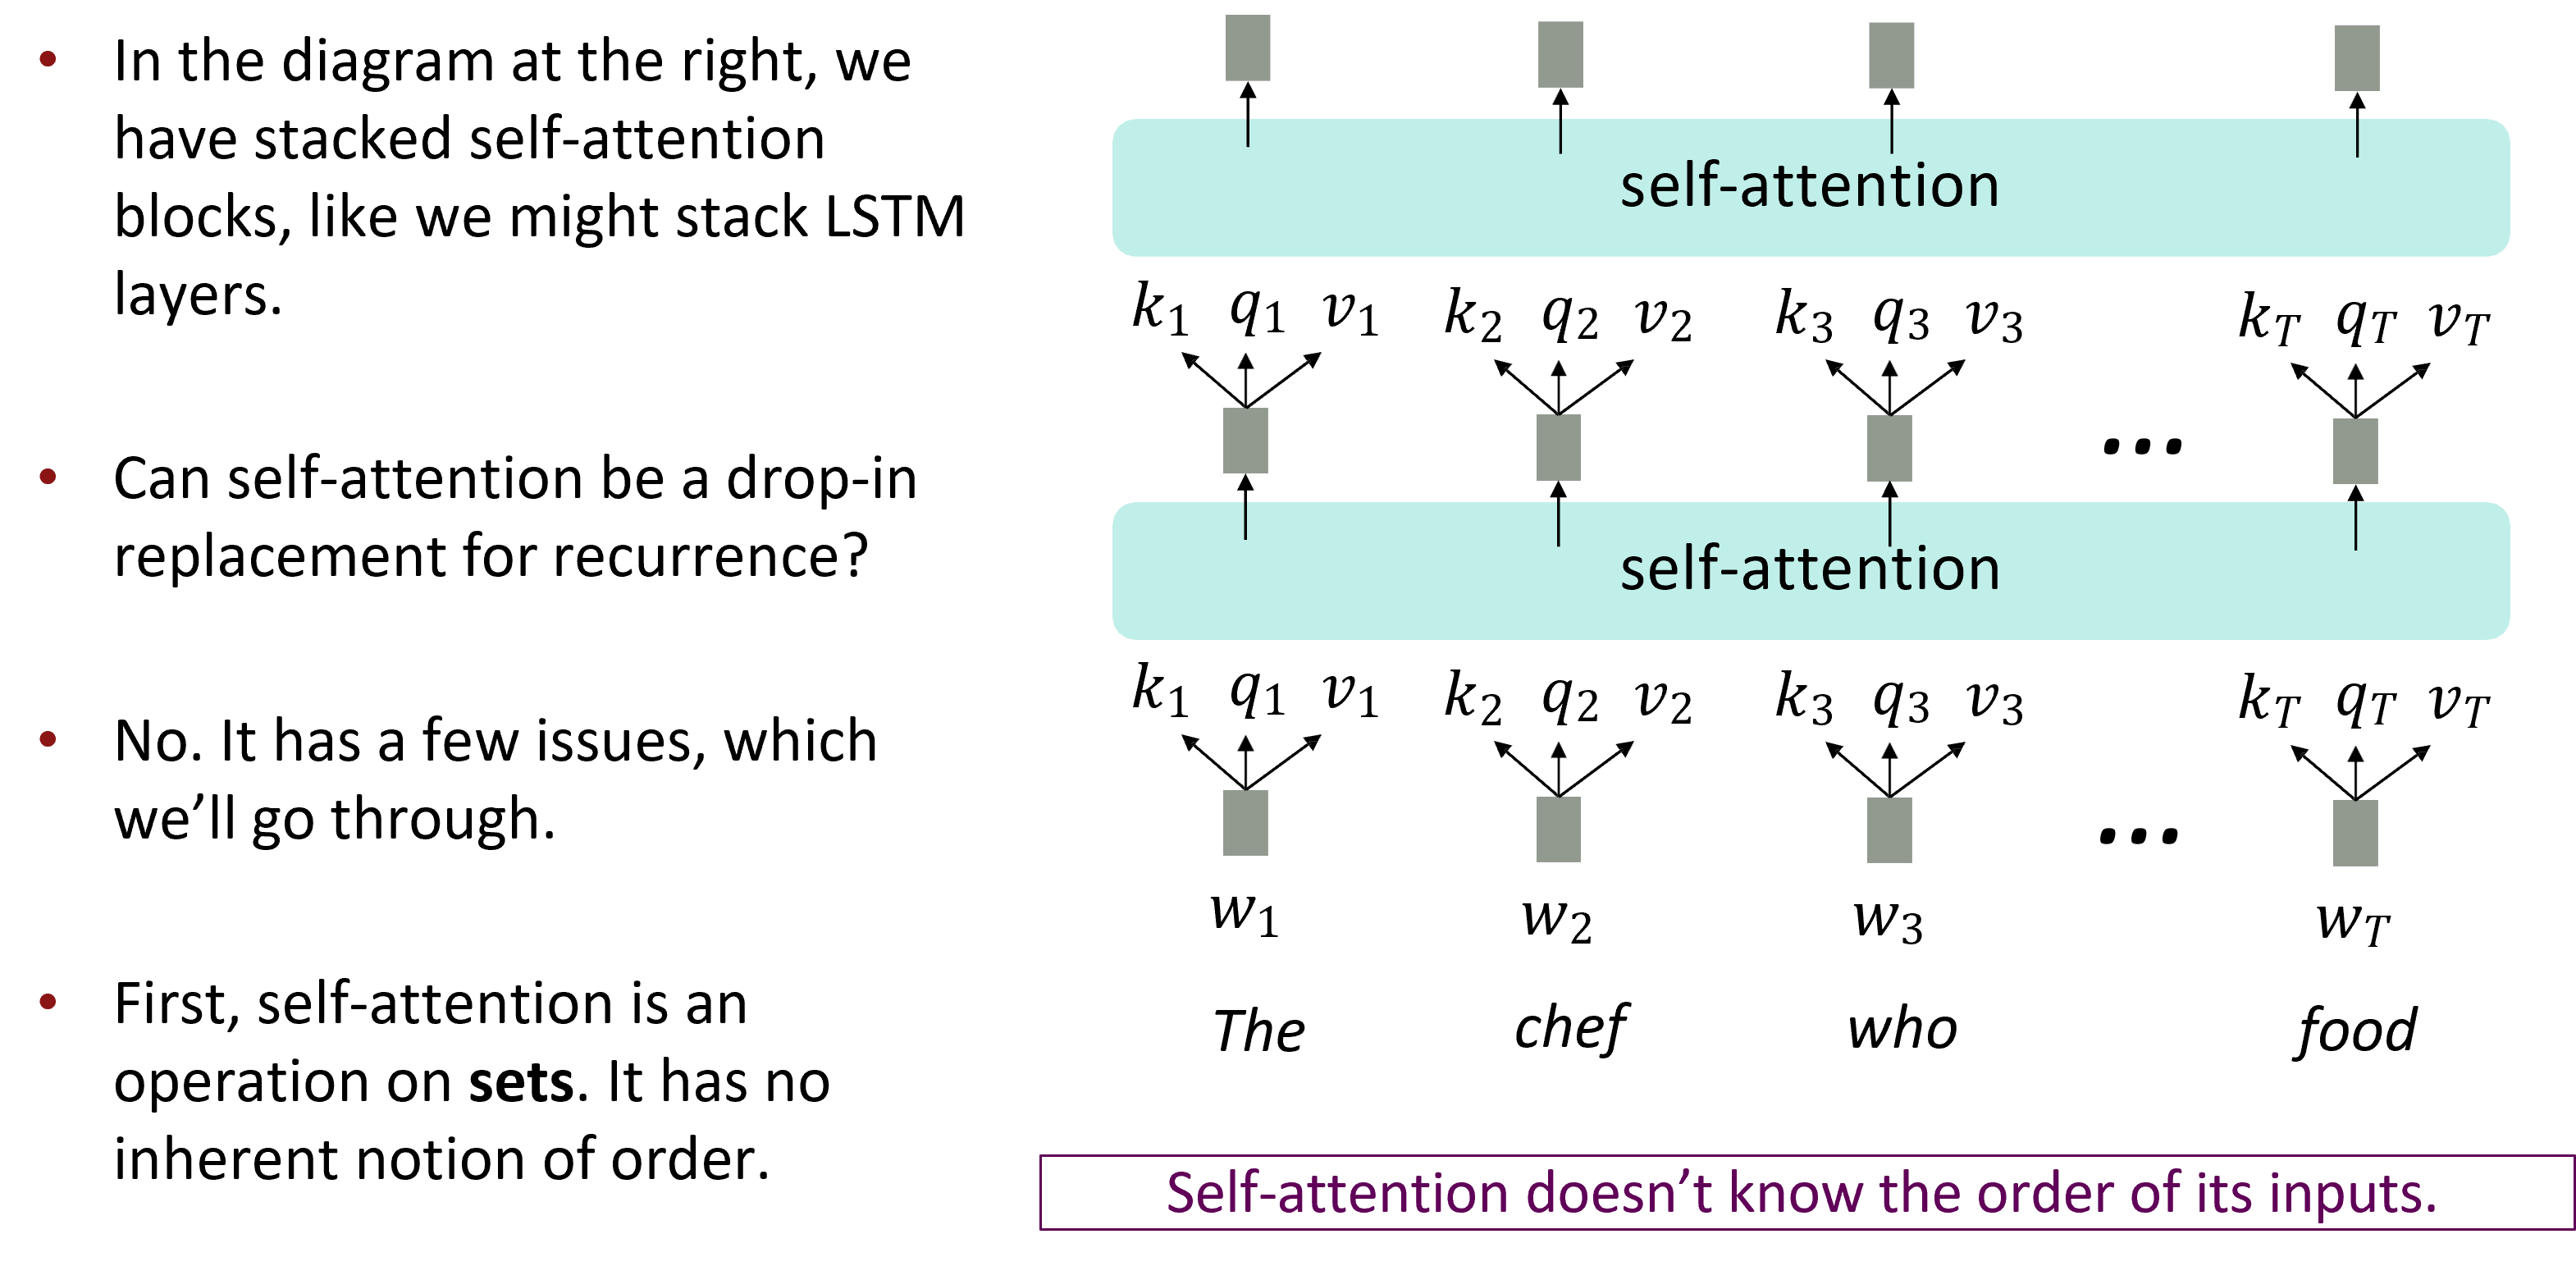
\includegraphics[width=\linewidth,keepaspectratio]{bert41}
\end{center}	

 
{\tiny (Ref: Language \& Machine Learning - John Hewitt)}
\end{frame}

%%%%%%%%%%%%%%%%%%%%%%%%%%%%%%%%%%%%%%%%%%%%%%%%%%%%%%%%%%%
\begin{frame}[fragile]\frametitle{Self-Attention}

Barriers and solutions for Self-Attention as a building block

\begin{center}
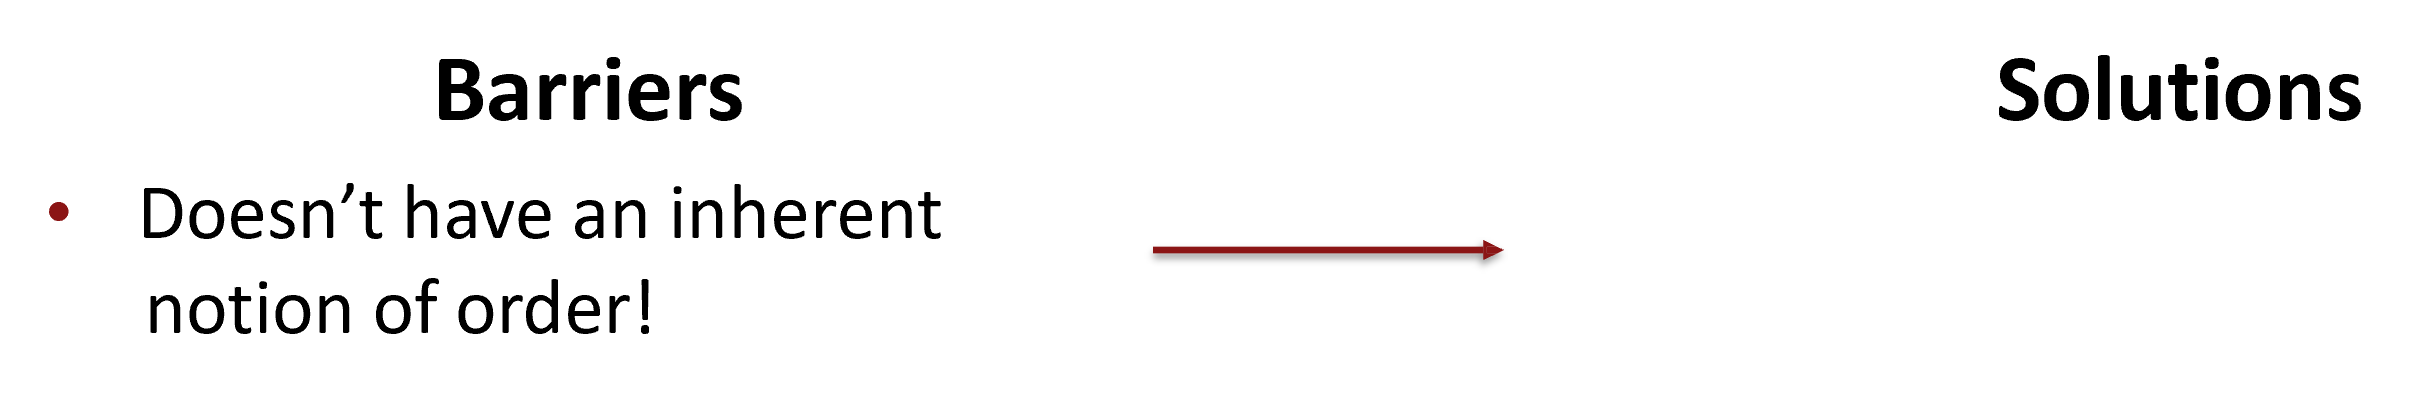
\includegraphics[width=\linewidth,keepaspectratio]{bert42}
\end{center}	

 
{\tiny (Ref: Language \& Machine Learning - John Hewitt)}
\end{frame}

%%%%%%%%%%%%%%%%%%%%%%%%%%%%%%%%%%%%%%%%%%%%%%%%%%%%%%%%%%%
\begin{frame}[fragile]\frametitle{Self-Attention}

Fixing the first self-attention problem: Sequence order

\begin{center}
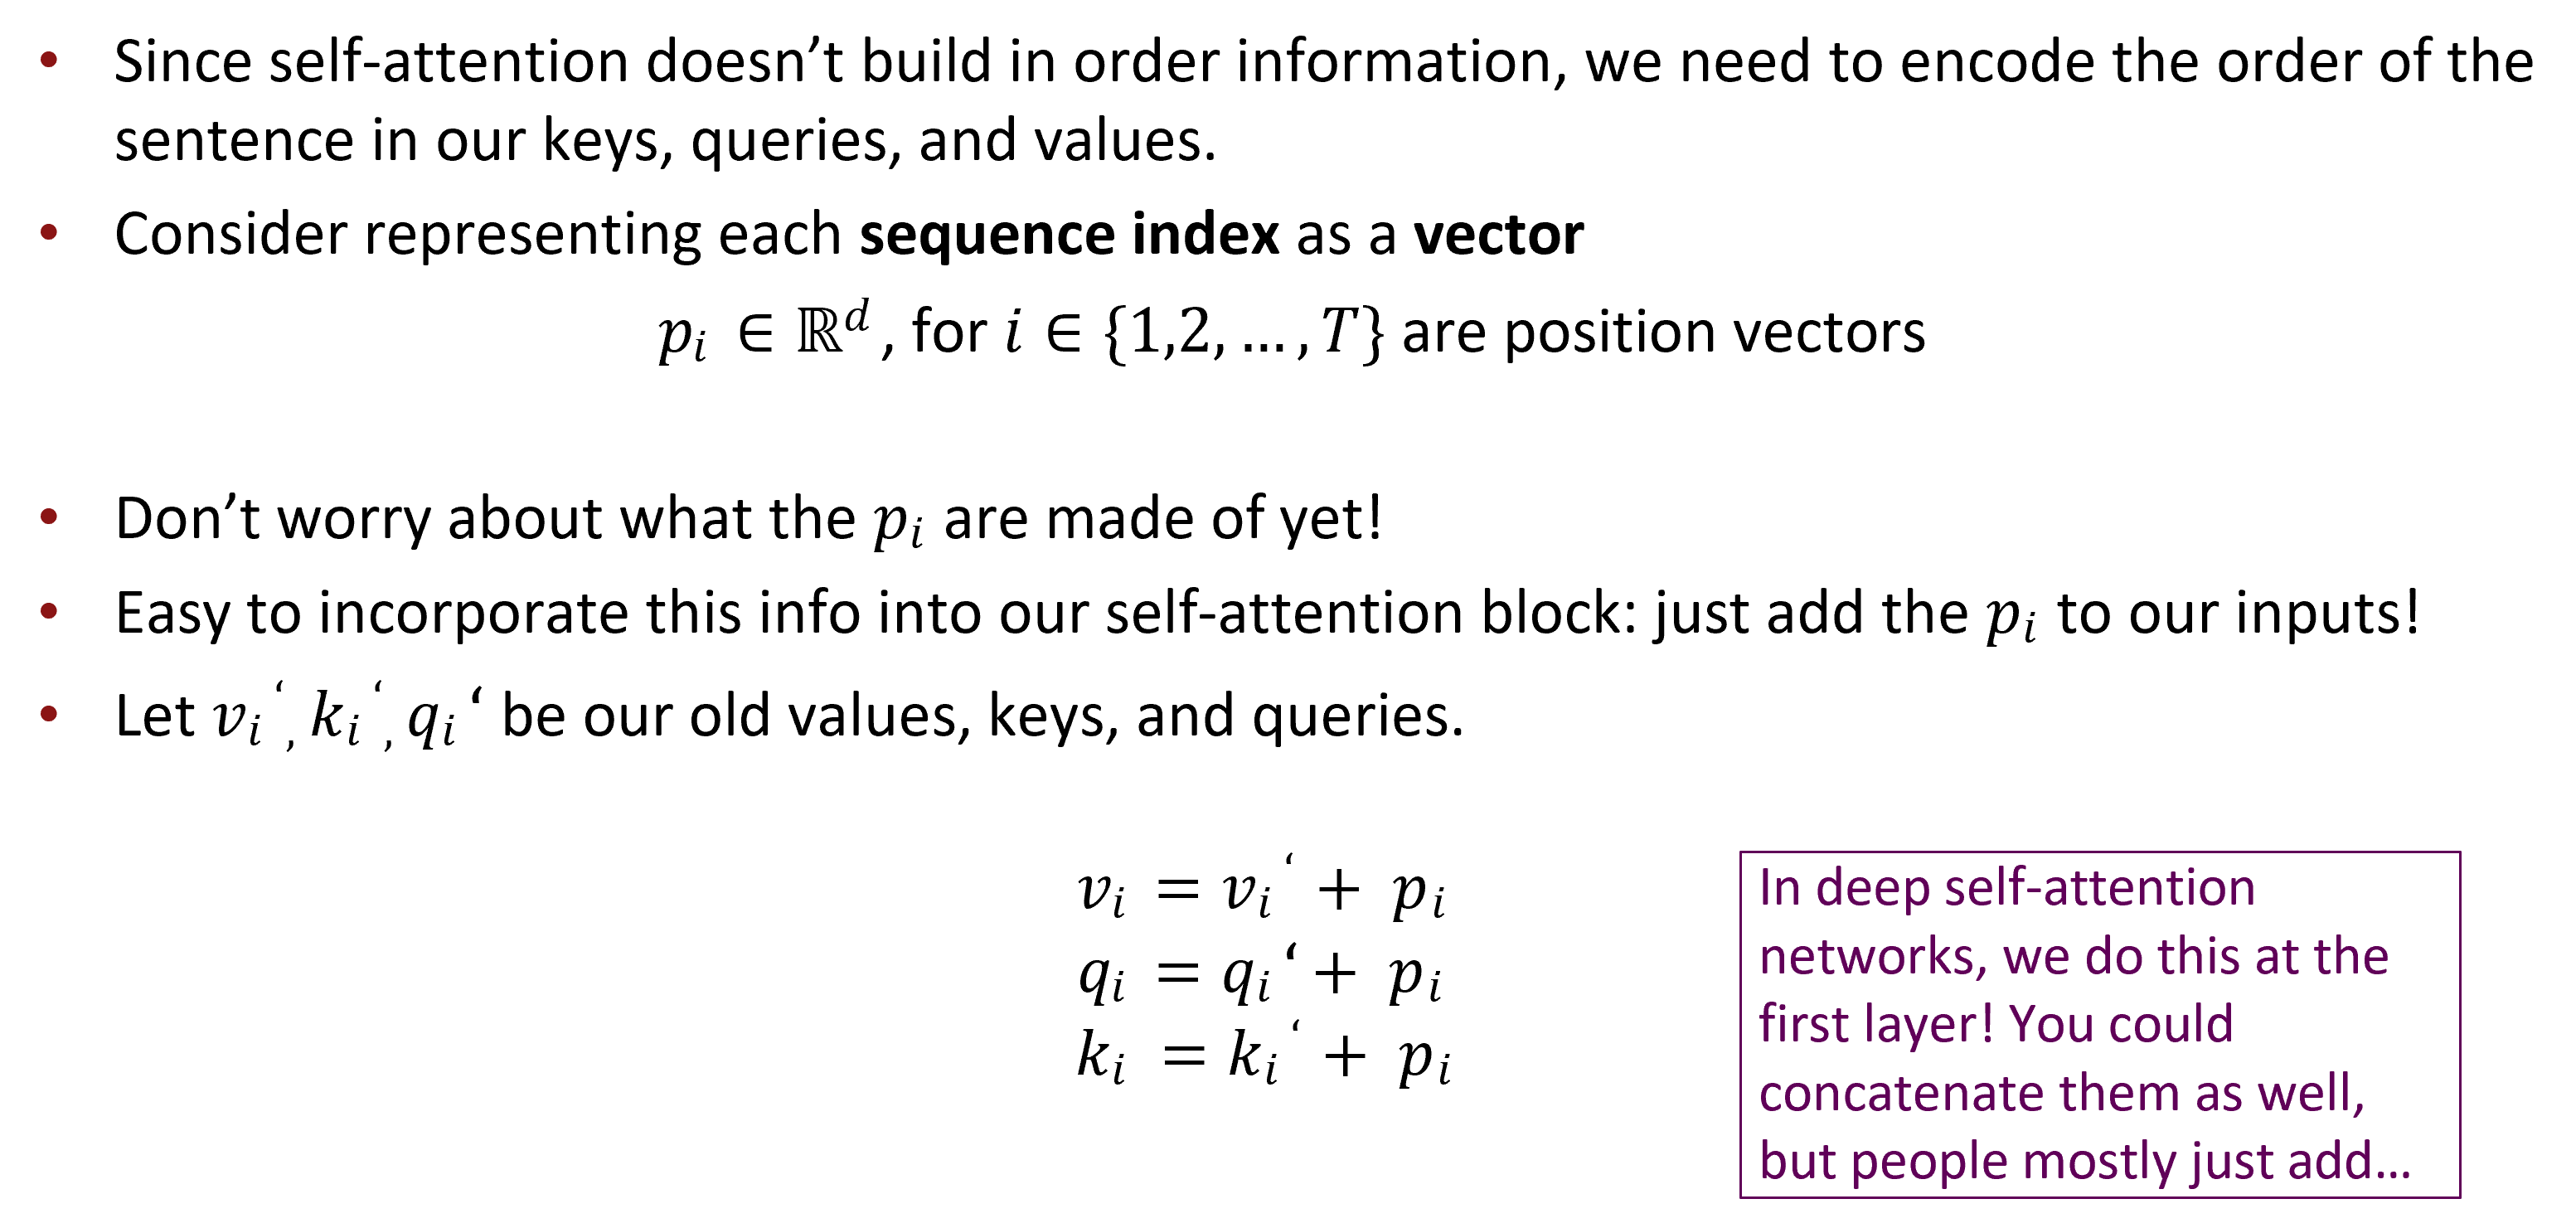
\includegraphics[width=\linewidth,keepaspectratio]{bert43}
\end{center}	

 
{\tiny (Ref: Language \& Machine Learning - John Hewitt)}
\end{frame}

%%%%%%%%%%%%%%%%%%%%%%%%%%%%%%%%%%%%%%%%%%%%%%%%%%%%%%%%%%%
\begin{frame}[fragile]\frametitle{Self-Attention}

Position representation vectors through sinusoids

\begin{center}
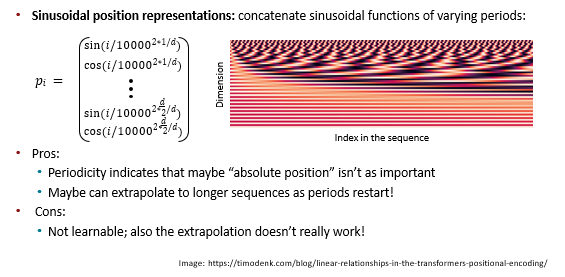
\includegraphics[width=\linewidth,keepaspectratio]{bert44}
\end{center}	

 
{\tiny (Ref: Language \& Machine Learning - John Hewitt)}
\end{frame}

%%%%%%%%%%%%%%%%%%%%%%%%%%%%%%%%%%%%%%%%%%%%%%%%%%%%%%%%%%%
\begin{frame}[fragile]\frametitle{Self-Attention}

Barriers and solutions for Self-Attention as a building block

\begin{center}
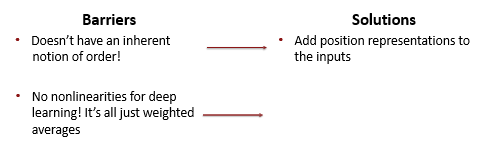
\includegraphics[width=\linewidth,keepaspectratio]{bert45}
\end{center}	

 
{\tiny (Ref: Language \& Machine Learning - John Hewitt)}
\end{frame}

%%%%%%%%%%%%%%%%%%%%%%%%%%%%%%%%%%%%%%%%%%%%%%%%%%%%%%%%%%%
\begin{frame}[fragile]\frametitle{Self-Attention}

Adding nonlinearities in self-attention

\begin{center}
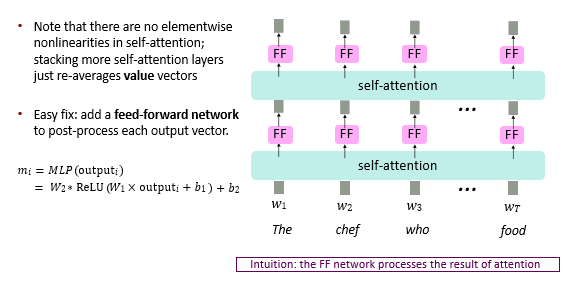
\includegraphics[width=\linewidth,keepaspectratio]{bert46}
\end{center}	

 
{\tiny (Ref: Language \& Machine Learning - John Hewitt)}
\end{frame}

%%%%%%%%%%%%%%%%%%%%%%%%%%%%%%%%%%%%%%%%%%%%%%%%%%%%%%%%%%%
\begin{frame}[fragile]\frametitle{Self-Attention}

Barriers and solutions for Self-Attention as a building block

\begin{center}
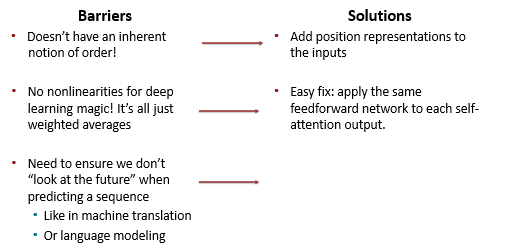
\includegraphics[width=\linewidth,keepaspectratio]{bert47}
\end{center}	

 
{\tiny (Ref: Language \& Machine Learning - John Hewitt)}
\end{frame}


%%%%%%%%%%%%%%%%%%%%%%%%%%%%%%%%%%%%%%%%%%%%%%%%%%%%%%%%%%%
\begin{frame}[fragile]\frametitle{Self-Attention}

Masking the future in self-attention

\begin{center}
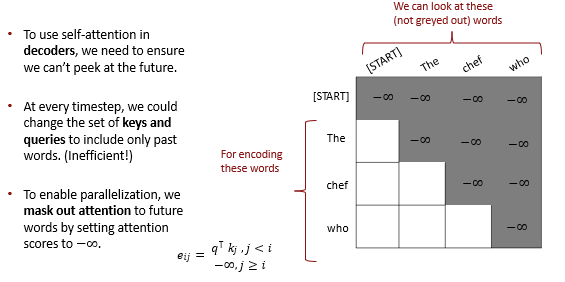
\includegraphics[width=\linewidth,keepaspectratio]{bert48}
\end{center}	

 
{\tiny (Ref: Language \& Machine Learning - John Hewitt)}
\end{frame}

%%%%%%%%%%%%%%%%%%%%%%%%%%%%%%%%%%%%%%%%%%%%%%%%%%%%%%%%%%%
\begin{frame}[fragile]\frametitle{Self-Attention}

Barriers and solutions for Self-Attention as a building block

\begin{center}
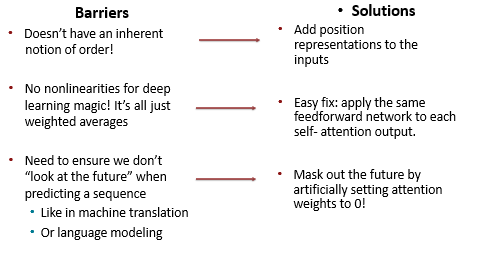
\includegraphics[width=\linewidth,keepaspectratio]{bert49}
\end{center}	

 
{\tiny (Ref: Language \& Machine Learning - John Hewitt)}
\end{frame}

%%%%%%%%%%%%%%%%%%%%%%%%%%%%%%%%%%%%%%%%%%%%%%%%%%%%%%%%%%%
\begin{frame}[fragile]\frametitle{Self-Attention}

Necessities for a self-attention building block:

\begin{itemize}
\item Self-attention:
the basis of the method.
\item Position representations:
Specify the sequence order, since self-attention is an unordered function of its  inputs.
\item Nonlinearities:
\begin{itemize}
\item At the output of the self-attention block
\item Frequently implemented as a simple feed-forward network.
\end{itemize}	 

\item Masking:
\begin{itemize}
\item In order to parallelize operations while not looking at the future.
\item Keeps information about the future from “leaking” to the past.
\end{itemize}	 

\item That’s it! But this is not the Transformer model we’ve been hearing about.


\end{itemize}	 

 
{\tiny (Ref: Language \& Machine Learning - John Hewitt)}
\end{frame}

%%%%%%%%%%%%%%%%%%%%%%%%%%%%%%%%%%%%%%%%%%%%%%%%%%%%%%%%%%%%%%%%%%%%%%%%%%%%%%%%%%
\begin{frame}[fragile]\frametitle{}
\begin{center}
{\Large Transformer \\ \small Attention is all you need}
\end{center}
\end{frame}


%%%%%%%%%%%%%%%%%%%%%%%%%%%%%%%%%%%%%%%%%%%%%%%%%%%%%%%%%%%
\begin{frame}[fragile]\frametitle{Popularity}

Masking the future in self-attention

\begin{center}
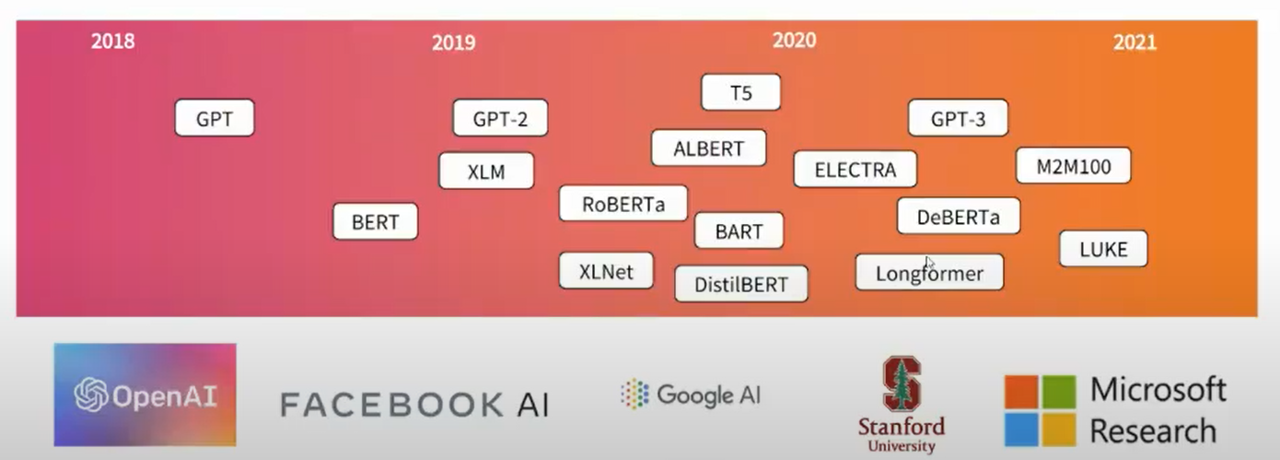
\includegraphics[width=\linewidth,keepaspectratio]{bert50}
\end{center}	

 
{\tiny (Ref: Niels Rogge on Huggingface contributions)}
\end{frame}


%%%%%%%%%%%%%%%%%%%%%%%%%%%%%%%%%%%%%%%%%%%%%%%%%%%%%%%%%%%
\begin{frame}[fragile]\frametitle{Transformers}


\begin{itemize}
\item The Transformer  is a model that uses attention to boost the speed with which seq2seq with attention models can be trained. The biggest benefit, however, comes from how The Transformer lends itself to parallelization. We will break it apart and look at how it functions.
\item In its heart it contains an encoding component, a decoding component, and connections between them.
\end{itemize}	 

\begin{center}
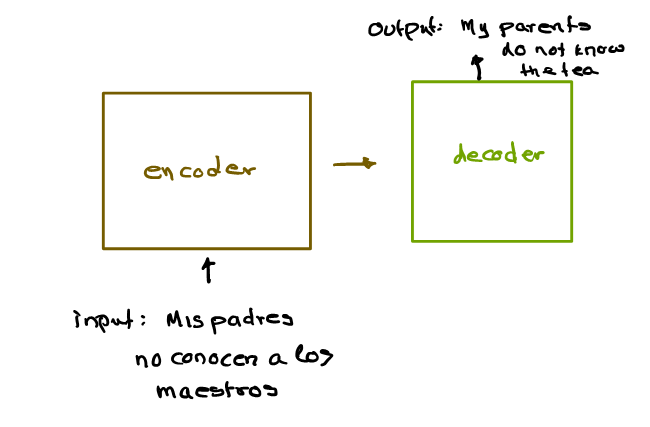
\includegraphics[width=0.5\linewidth,keepaspectratio]{bert51}
\end{center}	

\end{frame}


%%%%%%%%%%%%%%%%%%%%%%%%%%%%%%%%%%%%%%%%%%%%%%%%%%%%%%%%%%%
\begin{frame}[fragile]\frametitle{Transformers}
\begin{columns}
    \begin{column}[T]{0.5\linewidth}
      \begin{itemize}
			\item The encoding is a stack of encoders.
			\item The original paper stacks six of them on top of each other – there’s nothing magical about the number six, one can definitely experiment with other arrangements). 
			\item The decoding is a stack of decoders of the same number.
			\end{itemize}
		\end{column}
    \begin{column}[T]{0.5\linewidth}
		
			\begin{center}
			\includegraphics[width=0.8\linewidth,keepaspectratio]{bert52}
			\end{center}

    \end{column}
  \end{columns}
\end{frame}


%%%%%%%%%%%%%%%%%%%%%%%%%%%%%%%%%%%%%%%%%%%%%%%%%%%%%%%%%%%
\begin{frame}[fragile]\frametitle{Transformers}
\begin{columns}
    \begin{column}[T]{0.5\linewidth}
     The encoder’s inputs goes through a self-attention layer – a layer that helps the encoder look at other words in the input sentence as it encodes a specific word.  
		\end{column}
    \begin{column}[T]{0.5\linewidth}
		The decoder has both those layers, but between them is an attention layer that helps the decoder focus on relevant parts of the input sentence (similar what attention does in seq2seq models).
    \end{column}
  \end{columns}
	
			\begin{center}
			\includegraphics[width=0.8\linewidth,keepaspectratio]{bert53}
			\end{center}
			
\end{frame}

%%%%%%%%%%%%%%%%%%%%%%%%%%%%%%%%%%%%%%%%%%%%%%%%%%%%%%%%%%%
\begin{frame}[fragile]\frametitle{Transformers}
\begin{columns}
    \begin{column}[T]{0.5\linewidth}
			\begin{center}
			\includegraphics[width=0.8\linewidth,keepaspectratio]{bert58}
			\end{center}		
		\end{column}
    \begin{column}[T]{0.5\linewidth}
      \begin{itemize}
			\item A key property of the Transformer, which is that the word in each position flows through its own path in the encoder. There are dependencies between these paths in the self-attention layer. 
			\item The feed-forward layer does not have those dependencies, Therefore, the various paths can be executed in parallel while flowing through the feed-forward layer.
			\end{itemize}
    \end{column}
  \end{columns}
			
\end{frame}

%%%%%%%%%%%%%%%%%%%%%%%%%%%%%%%%%%%%%%%%%%%%%%%%%%%%%%%%%%%
\begin{frame}[fragile]\frametitle{Transformers}
Patrick was not late for class because {\bf he} is a responsible student

\begin{columns}
    \begin{column}[T]{0.5\linewidth}
			\begin{center}
			\includegraphics[width=0.8\linewidth,keepaspectratio]{bert54}
			\end{center}		
		\end{column}
    \begin{column}[T]{0.5\linewidth}
      \begin{itemize}
			\item What does ``he'' in this sentence refer to? Is it referring to the class or to the student? It's a simple question to a human, but not as simple to an algorithm.
			\item When the model is processing the word ``he'', self-attention allows it to associate ``he'' with ``Patrick''.
			\end{itemize}
    \end{column}
  \end{columns}
			
\end{frame}

%%%%%%%%%%%%%%%%%%%%%%%%%%%%%%%%%%%%%%%%%%%%%%%%%%%%%%%%%%%
\begin{frame}[fragile]\frametitle{Transformers}
	\begin{center}
	\includegraphics[width=0.8\linewidth,keepaspectratio]{bert55}
	\end{center}	
\end{frame}

%%%%%%%%%%%%%%%%%%%%%%%%%%%%%%%%%%%%%%%%%%%%%%%%%%%%%%%%%%%
\begin{frame}[fragile]\frametitle{Transformers}

\begin{columns}
    \begin{column}[T]{0.5\linewidth}
			\begin{center}
			\includegraphics[width=0.8\linewidth,keepaspectratio]{bert60}
			\end{center}		
		\end{column}
    \begin{column}[T]{0.5\linewidth}
		In the same fashion as CNN that we need more than one filter, transformers add a mechanism called ``multi-headed'' attention. This improves the performance of the attention layer in two ways:

      \begin{itemize}
			\item It expands the model's ability to focus on different positions.
			\item It gives the attention layer multiple ``representation subspaces''
			\end{itemize}
    \end{column}
  \end{columns}
			
\end{frame}

%%%%%%%%%%%%%%%%%%%%%%%%%%%%%%%%%%%%%%%%%%%%%%%%%%%%%%%%%%%
\begin{frame}[fragile]\frametitle{Transformers}

\begin{columns}
    \begin{column}[T]{0.5\linewidth}
			\begin{center}
			\includegraphics[width=0.8\linewidth,keepaspectratio]{bert56}
			\end{center}		
		\end{column}
    \begin{column}[T]{0.5\linewidth}
As we encode the word ”he", one attention head is focusing most on ``Patrick'', while another is focusing on ``student'' -- in a sense, the model's representation of the word ``he'' combines the representations of both ``Patrick'' and ``stduent''.

    \end{column}
  \end{columns}
			
\end{frame}

%%%%%%%%%%%%%%%%%%%%%%%%%%%%%%%%%%%%%%%%%%%%%%%%%%%%%%%%%%%
\begin{frame}[fragile]\frametitle{Transformers}


			\begin{center}
			\includegraphics[width=0.8\linewidth,keepaspectratio]{bert57}
			\end{center}		

			
\end{frame}


%%%%%%%%%%%%%%%%%%%%%%%%%%%%%%%%%%%%%%%%%%%%%%%%%%%%%%%%%%%
\begin{frame}[fragile]\frametitle{Transformers}

\begin{columns}
    \begin{column}[T]{0.5\linewidth}
			\begin{center}
			\includegraphics[width=0.8\linewidth,keepaspectratio]{bert61}
			\end{center}		
		\end{column}
    \begin{column}[T]{0.5\linewidth}
      \begin{itemize}
			\item Details in the architecture of the encoder:
			\item Each sub-layer  in each encoder has a residual connection around it
			\item And a layer-normalization step.
			\end{itemize}
    \end{column}
  \end{columns}
			
\end{frame}

%%%%%%%%%%%%%%%%%%%%%%%%%%%%%%%%%%%%%%%%%%%%%%%%%%%%%%%%%%%
\begin{frame}[fragile]\frametitle{Transformers}


			\begin{center}
			\includegraphics[width=0.8\linewidth,keepaspectratio]{bert62}
			\end{center}		

			
\end{frame}

%%%%%%%%%%%%%%%%%%%%%%%%%%%%%%%%%%%%%%%%%%%%%%%%%%%%%%%%%%%
\begin{frame}[fragile]\frametitle{Transformers}


			\begin{center}
			\includegraphics[width=0.8\linewidth,keepaspectratio]{bert63}
			\end{center}		

			
\end{frame}

%%%%%%%%%%%%%%%%%%%%%%%%%%%%%%%%%%%%%%%%%%%%%%%%%%%%%%%%%%%
\begin{frame}[fragile]\frametitle{The Final Linear and Softmax Layer}


			\begin{center}
			\includegraphics[width=0.8\linewidth,keepaspectratio]{bert64}
			\end{center}		

			
\end{frame}

%%%%%%%%%%%%%%%%%%%%%%%%%%%%%%%%%%%%%%%%%%%%%%%%%%%%%%%%%%%
\begin{frame}[fragile]\frametitle{Architecture}

\begin{columns}
    \begin{column}[T]{0.5\linewidth}
			\begin{center}
			\includegraphics[width=0.8\linewidth,keepaspectratio]{bert65}
			\end{center}		
		\end{column}
    \begin{column}[T]{0.5\linewidth}
      \begin{itemize}
			\item Encoder-Decoder was there
			\item New?: Multi head attention
			\item Fine tuned with Custom Data
			\item Flavors:
      \begin{itemize}
			\item Encoder only: BERT, XLNet
			\item Decoder only
			\item Encoder-Decoder
			\end{itemize}
			\end{itemize}
    \end{column}
  \end{columns}
			
\end{frame}

%%%%%%%%%%%%%%%%%%%%%%%%%%%%%%%%%%%%%%%%%%%%%%%%%%%%%%%%%%%
\begin{frame}[fragile]\frametitle{Encoder only}

\begin{columns}
    \begin{column}[T]{0.5\linewidth}
			\begin{center}
			\includegraphics[width=0.8\linewidth,keepaspectratio]{bert66}
			\end{center}		
		\end{column}
    \begin{column}[T]{0.5\linewidth}
      \begin{itemize}
			\item If we are only interested in training a language model for the input for some other tasks, then we do not need the decoder of the transformer. 
			\item Pre-trained by predicting masked word
			\item BERT, XLNet, DistillBERT, RoBERTA
			\item Usage:
      \begin{itemize}
			\item Text Classification
			\item Named Entity Recognition
			\item Extractive Question Answering
			\end{itemize}
			\end{itemize}
    \end{column}
  \end{columns}
			
\end{frame}

%%%%%%%%%%%%%%%%%%%%%%%%%%%%%%%%%%%%%%%%%%%%%%%%%%%%%%%%%%%
\begin{frame}[fragile]\frametitle{Decoder only}

\begin{columns}
    \begin{column}[T]{0.5\linewidth}
			\begin{center}
			\includegraphics[width=0.8\linewidth,keepaspectratio]{bert67}
			\end{center}		
		\end{column}
    \begin{column}[T]{0.5\linewidth}
      \begin{itemize}
			\item If we do not have input, we just want to model the “next word”, we can get rid of the encoder side of a transformer and output “next word” one by one. 
			\item Pre-trained by predicting next word
			\item GPT-*, Transformer XL
			\item Usage:
      \begin{itemize}
			\item Text Generation
			\end{itemize}
			\end{itemize}
    \end{column}
  \end{columns}
			
\end{frame}

%%%%%%%%%%%%%%%%%%%%%%%%%%%%%%%%%%%%%%%%%%%%%%%%%%%%%%%%%%%
\begin{frame}[fragile]\frametitle{Encoder-Decoder, both}

\begin{columns}
    \begin{column}[T]{0.5\linewidth}
			\begin{center}
			\includegraphics[width=0.8\linewidth,keepaspectratio]{bert68}
			\end{center}		
		\end{column}
    \begin{column}[T]{0.5\linewidth}
      \begin{itemize}
			\item Pre-trained by Seq2Seq manner
			\item T5, BART, PEGASUS
			\item Usage:
      \begin{itemize}
			\item Text summarization
			\item Machine Translation
			\item SQL generation
			\end{itemize}
			\end{itemize}
    \end{column}
  \end{columns}
			
\end{frame}

%%%%%%%%%%%%%%%%%%%%%%%%%%%%%%%%%%%%%%%%%%%%%%%%%%%%%%%%%%%
\begin{frame}[fragile]\frametitle{Transformer Overview}

\begin{columns}
    \begin{column}[T]{0.5\linewidth}
			\begin{center}
			\includegraphics[width=0.8\linewidth,keepaspectratio]{bert69}
			\end{center}		
		\end{column}
    \begin{column}[T]{0.5\linewidth}
		Attention is all you need. 2017.  Aswani, Shazeer, Parmar, Uszkoreit,  Jones, Gomez, Kaiser, Polosukhin  https://arxiv.org/pdf/1706.03762.pdf 

      \begin{itemize}
			\item Non-recurrent sequence-to-  sequence encoder-decoder model
			\item Task: machine translation  with parallel corpus
			\item Predict each translated word
			\item Final cost/error function is  standard cross-entropy error on top of a softmax classifier
			\end{itemize}
    \end{column}
  \end{columns}
			
\end{frame}

%%%%%%%%%%%%%%%%%%%%%%%%%%%%%%%%%%%%%%%%%%%%%%%%%%%%%%%%%%%
\begin{frame}[fragile]\frametitle{Transformer Encoder}

\begin{columns}
    \begin{column}[T]{0.5\linewidth}
			\begin{center}
			\includegraphics[width=0.6\linewidth,keepaspectratio]{bert70}
			\end{center}		
		\end{column}
    \begin{column}[T]{0.5\linewidth}
      \begin{itemize}
			\item For encoder, at each block, we use the same Q, K and V; from the previous layer
			\item Blocks are repeated 6 times (in vertical stack)
			\end{itemize}
    \end{column}
  \end{columns}
			
\end{frame}

%%%%%%%%%%%%%%%%%%%%%%%%%%%%%%%%%%%%%%%%%%%%%%%%%%%%%%%%%%%
\begin{frame}[fragile]\frametitle{Transformer Decoder}


			\begin{center}
			\includegraphics[width=\linewidth,keepaspectratio]{bert71}
			\end{center}		

			
\end{frame}

%%%%%%%%%%%%%%%%%%%%%%%%%%%%%%%%%%%%%%%%%%%%%%%%%%%%%%%%%%%
\begin{frame}[fragile]\frametitle{Transformer Encoder-Decoder}

			\begin{center}
			\includegraphics[width=\linewidth,keepaspectratio]{bert72}
			\end{center}		

			
\end{frame}

%%%%%%%%%%%%%%%%%%%%%%%%%%%%%%%%%%%%%%%%%%%%%%%%%%%%%%%%%%%
\begin{frame}[fragile]\frametitle{Transformer Encoder-Decoder}
Next, let’s look at the Transformer Encoder and Decoder Blocks

What’s left in a Transformer Encoder Block that we haven’t covered?

      \begin{itemize}
			\item Key-query-value attention: How do we get the $k,q,v$ vectors from a single word embedding?
			\item Multi-headed attention: Attend to multiple places in a single layer!
			\item Tricks to help with training!
			    \begin{itemize}
					\item Residual connections
					\item Layer normalization
					\item Scaling the dot product
					\item These tricks don’t improve what the model is able to do; they help improve the training process
					\end{itemize}

			\end{itemize}
			
\end{frame}

%%%%%%%%%%%%%%%%%%%%%%%%%%%%%%%%%%%%%%%%%%%%%%%%%%%%%%%%%%%
\begin{frame}[fragile]\frametitle{The Transformer Encoder: Dot-Product Attention}


      \begin{itemize}
			\item Inputs: a query q and a set of key-value (k-v) pairs to an output
			\item Query, keys, values, and output are all vectors
			\item Output is weighted sum of values, where
			\item Weight of each value is computed by an inner product of query and corresponding key
			\item Queries and keys have same dimensionality $d_k$ , value have $d_v$
			\end{itemize}
			
			\begin{center}
			\includegraphics[width=0.6\linewidth,keepaspectratio]{bert73}
			\end{center}		
			
			{\tiny (Ref: CS224n: Natural Language Processing with Deep Learning - Christopher Manning)}

\end{frame}

%%%%%%%%%%%%%%%%%%%%%%%%%%%%%%%%%%%%%%%%%%%%%%%%%%%%%%%%%%%
\begin{frame}[fragile]\frametitle{The Transformer Encoder: Dot-Product Attention: Matrix notation}


      \begin{itemize}
			\item Inputs: a query q and a set of key-value (k-v) pairs to an output
			\item Query, keys, values, and output are all vectors
			\item Output is weighted sum of values, where
			\item Weight of each value is computed by an inner product of query and corresponding key
			\item Queries and keys have same dimensionality $d_k$ , value have $d_v$
			\end{itemize}
			
			\begin{center}
			\includegraphics[width=0.6\linewidth,keepaspectratio]{bert74}
			\end{center}		
			
			{\tiny (Ref: CS224n: Natural Language Processing with Deep Learning - Christopher Manning)}

\end{frame}

%%%%%%%%%%%%%%%%%%%%%%%%%%%%%%%%%%%%%%%%%%%%%%%%%%%%%%%%%%%
\begin{frame}[fragile]\frametitle{The Transformer Encoder: Key-Query-Value Attention}

			
			\begin{center}
			\includegraphics[width=\linewidth,keepaspectratio]{bert75}
			\end{center}		
			
{\tiny (Ref: Language \& Machine Learning - John Hewitt)}

\end{frame}

%%%%%%%%%%%%%%%%%%%%%%%%%%%%%%%%%%%%%%%%%%%%%%%%%%%%%%%%%%%
\begin{frame}[fragile]\frametitle{The Transformer Encoder: Key-Query-Value Attention}

			
			\begin{center}
			\includegraphics[width=\linewidth,keepaspectratio]{bert76}
			\end{center}		
			
{\tiny (Ref: Language \& Machine Learning - John Hewitt)}

\end{frame}

%%%%%%%%%%%%%%%%%%%%%%%%%%%%%%%%%%%%%%%%%%%%%%%%%%%%%%%%%%%
\begin{frame}[fragile]\frametitle{The Transformer Encoder: Multi-headed attention}

			
			\begin{center}
			\includegraphics[width=\linewidth,keepaspectratio]{bert77}
			\end{center}		
			
{\tiny (Ref: Language \& Machine Learning - John Hewitt)}

\end{frame}

%%%%%%%%%%%%%%%%%%%%%%%%%%%%%%%%%%%%%%%%%%%%%%%%%%%%%%%%%%%
\begin{frame}[fragile]\frametitle{The Transformer Encoder: Multi-headed attention}

			
			\begin{center}
			\includegraphics[width=\linewidth,keepaspectratio]{bert78}
			\end{center}		
			
{\tiny (Ref: Language \& Machine Learning - John Hewitt)}

\end{frame}

%%%%%%%%%%%%%%%%%%%%%%%%%%%%%%%%%%%%%%%%%%%%%%%%%%%%%%%%%%%
\begin{frame}[fragile]\frametitle{Attention visualization in layer 5}

			
			\begin{center}
			\includegraphics[width=\linewidth,keepaspectratio]{bert79}
			\end{center}		
			
			{\tiny (Ref: CS224n: Natural Language Processing with Deep Learning - Christopher Manning)}

\end{frame}

%%%%%%%%%%%%%%%%%%%%%%%%%%%%%%%%%%%%%%%%%%%%%%%%%%%%%%%%%%%
\begin{frame}[fragile]\frametitle{Attention visualization: Implicit anaphora resolution}

			
			\begin{center}
			\includegraphics[width=\linewidth,keepaspectratio]{bert80}
			\end{center}		
			
			In 5th layer. Isolated attentions from just the word ‘its’ for attention heads 5 and 6.  Note that the attentions are very sharp for this word.

			
			{\tiny (Ref: CS224n: Natural Language Processing with Deep Learning - Christopher Manning)}

\end{frame}

%%%%%%%%%%%%%%%%%%%%%%%%%%%%%%%%%%%%%%%%%%%%%%%%%%%%%%%%%%%
\begin{frame}[fragile]\frametitle{Parallel attention heads}

			
			\begin{center}
			\includegraphics[width=0.8\linewidth,keepaspectratio]{bert81}
			\end{center}		
			
		
			{\tiny (Ref: Ashish Vaswani)}

\end{frame}

%%%%%%%%%%%%%%%%%%%%%%%%%%%%%%%%%%%%%%%%%%%%%%%%%%%%%%%%%%%
\begin{frame}[fragile]\frametitle{The Transformer Encoder: Residual connections [He et al., 2016]}

			
			\begin{center}
			\includegraphics[width=0.8\linewidth,keepaspectratio]{bert82}
			\end{center}		
			
		
			{\tiny (Ref: John Hewitt)}

\end{frame}

%%%%%%%%%%%%%%%%%%%%%%%%%%%%%%%%%%%%%%%%%%%%%%%%%%%%%%%%%%%
\begin{frame}[fragile]\frametitle{The Transformer Encoder: Layer normalization [Ba et al., 2016]}

			
			\begin{center}
			\includegraphics[width=0.8\linewidth,keepaspectratio]{bert83}
			\end{center}		
			
		
			{\tiny (Ref: John Hewitt)}

\end{frame}

%%%%%%%%%%%%%%%%%%%%%%%%%%%%%%%%%%%%%%%%%%%%%%%%%%%%%%%%%%%
\begin{frame}[fragile]\frametitle{The Transformer Encoder: Scaled Dot Product [Vaswani et al., 2017]}

			
			\begin{center}
			\includegraphics[width=0.8\linewidth,keepaspectratio]{bert84}
			\end{center}		
			
		
			{\tiny (Ref: John Hewitt)}

\end{frame}

%%%%%%%%%%%%%%%%%%%%%%%%%%%%%%%%%%%%%%%%%%%%%%%%%%%%%%%%%%%
\begin{frame}[fragile]\frametitle{The Transformer Encoder: Scaled Dot Product [Vaswani et al., 2017]}

			
			\begin{center}
			\includegraphics[width=0.8\linewidth,keepaspectratio]{bert85}
			\end{center}		
			
		
			{\tiny (Ref: John Hewitt)}

\end{frame}

%%%%%%%%%%%%%%%%%%%%%%%%%%%%%%%%%%%%%%%%%%%%%%%%%%%%%%%%%%%
\begin{frame}[fragile]\frametitle{The Transformer Encoder: Scaled Dot Product [Vaswani et al., 2017]}

			
			\begin{center}
			\includegraphics[width=0.8\linewidth,keepaspectratio]{bert86}
			\end{center}		
			
		
			{\tiny (Ref: John Hewitt)}

\end{frame}

%%%%%%%%%%%%%%%%%%%%%%%%%%%%%%%%%%%%%%%%%%%%%%%%%%%%%%%%%%%
\begin{frame}[fragile]\frametitle{The Transformer Encoder: Scaled Dot Product [Vaswani et al., 2017]}

			
			\begin{center}
			\includegraphics[width=0.8\linewidth,keepaspectratio]{bert87}
			\end{center}		
			
		
			{\tiny (Ref: John Hewitt)}

\end{frame}

%%%%%%%%%%%%%%%%%%%%%%%%%%%%%%%%%%%%%%%%%%%%%%%%%%%%%%%%%%%
\begin{frame}[fragile]\frametitle{The Transformer Encoder: Scaled Dot Product [Vaswani et al., 2017]}

			
			\begin{center}
			\includegraphics[width=0.8\linewidth,keepaspectratio]{bert88}
			\end{center}		
			
		
			{\tiny (Ref: John Hewitt)}

\end{frame}

%%%%%%%%%%%%%%%%%%%%%%%%%%%%%%%%%%%%%%%%%%%%%%%%%%%%%%%%%%%
\begin{frame}[fragile]\frametitle{The Transformer Decoder: Cross-attention (details)}

			
			\begin{center}
			\includegraphics[width=0.8\linewidth,keepaspectratio]{bert89}
			\end{center}		
			
		
			{\tiny (Ref: John Hewitt)}

\end{frame}

%%%%%%%%%%%%%%%%%%%%%%%%%%%%%%%%%%%%%%%%%%%%%%%%%%%%%%%%%%%
\begin{frame}[fragile]\frametitle{The Transformer Decoder: Cross-attention (details)}

			
			\begin{center}
			\includegraphics[width=0.8\linewidth,keepaspectratio]{bert90}
			\end{center}		
			
			{\tiny (Ref: John Hewitt)}

\end{frame}

%%%%%%%%%%%%%%%%%%%%%%%%%%%%%%%%%%%%%%%%%%%%%%%%%%%%%%%%%%%
\begin{frame}[fragile]\frametitle{Great Results with Transformers}

			
			\begin{center}
			\includegraphics[width=0.8\linewidth,keepaspectratio]{bert91}
			\end{center}		
			
			{\tiny (Ref: John Hewitt)}

\end{frame}

%%%%%%%%%%%%%%%%%%%%%%%%%%%%%%%%%%%%%%%%%%%%%%%%%%%%%%%%%%%
\begin{frame}[fragile]\frametitle{What would we like to fix about the Transformer?}

      \begin{itemize}
			\item Quadratic compute in self-attention:
			      \begin{itemize}
						\item Computing all pairs of interactions means our computation grows quadratically with the sequence length!
						\item For recurrent models, it only grew linearly!
						\end{itemize}
			\item Position representations:
			      \begin{itemize}
						\item Are simple absolute indices the best we can do to represent position?
						\item Relative linear position attention [Shaw et al., 2018]
						\item Dependency syntax-based position [Wang et al., 2019]			
						\end{itemize}
			\end{itemize}

			{\tiny (Ref: John Hewitt)}

\end{frame}

%%%%%%%%%%%%%%%%%%%%%%%%%%%%%%%%%%%%%%%%%%%%%%%%%%%%%%%%%%%
\begin{frame}[fragile]\frametitle{Quadratic computation as function of seq. length}

			
			\begin{center}
			\includegraphics[width=0.8\linewidth,keepaspectratio]{bert92}
			\end{center}		
			
			{\tiny (Ref: John Hewitt)}

\end{frame}

%%%%%%%%%%%%%%%%%%%%%%%%%%%%%%%%%%%%%%%%%%%%%%%%%%%%%%%%%%%
\begin{frame}[fragile]\frametitle{Recent work on improving on quadratic self-attention cost}

			
			\begin{center}
			\includegraphics[width=0.8\linewidth,keepaspectratio]{bert93}
			\end{center}		
			
			{\tiny (Ref: John Hewitt)}

\end{frame}

%%%%%%%%%%%%%%%%%%%%%%%%%%%%%%%%%%%%%%%%%%%%%%%%%%%%%%%%%%%
\begin{frame}[fragile]\frametitle{Recent work on improving on quadratic self-attention cost}

			
			\begin{center}
			\includegraphics[width=0.8\linewidth,keepaspectratio]{bert94}
			\end{center}		
			
			{\tiny (Ref: John Hewitt)}

\end{frame}

%%%%%%%%%%%%%%%%%%%%%%%%%%%%%%%%%%%%%%%%%%%%%%%%%%%%%%%%%%%
\begin{frame}[fragile]\frametitle{Recent work on improving on quadratic self-attention cost}

			
			\begin{center}
			\includegraphics[width=0.8\linewidth,keepaspectratio]{bert95}
			\end{center}		
			
			{\tiny (Ref: John Hewitt)}

\end{frame}

%%%%%%%%%%%%%%%%%%%%%%%%%%%%%%%%%%%%%%%%%%%%%%%%%%%%%%%%%%%
\begin{frame}[fragile]\frametitle{Pretraining models}

			
			\begin{center}
			\includegraphics[width=0.8\linewidth,keepaspectratio]{bert96}
			\end{center}		
			
			{\tiny (Ref: John Hewitt)}

\end{frame}

%%%%%%%%%%%%%%%%%%%%%%%%%%%%%%%%%%%%%%%%%%%%%%%%%%%%%%%%%%%
\begin{frame}[fragile]\frametitle{Pretraining through language modeling [Dai and Le, 2015]}

			
			\begin{center}
			\includegraphics[width=0.8\linewidth,keepaspectratio]{bert97}
			\end{center}		
			
			{\tiny (Ref: John Hewitt)}

\end{frame}

%%%%%%%%%%%%%%%%%%%%%%%%%%%%%%%%%%%%%%%%%%%%%%%%%%%%%%%%%%%
\begin{frame}[fragile]\frametitle{The Pretraining / Finetuning Paradigm}

			
			\begin{center}
			\includegraphics[width=0.8\linewidth,keepaspectratio]{bert98}
			\end{center}		
			
			{\tiny (Ref: John Hewitt)}

\end{frame}

%%%%%%%%%%%%%%%%%%%%%%%%%%%%%%%%%%%%%%%%%%%%%%%%%%%%%%%%%%%
\begin{frame}[fragile]\frametitle{Capturing meaning via context: What kinds of things does pretraining learn?}

There’s increasing evidence that pretrained models learn a wide variety of things about
the statistical properties of language:

      \begin{itemize}
			\item Stanford University is located in $---------$, California. [Trivia]
			\item I put $---------$ fork down on the table. [syntax]
			\item The woman walked across the street, checking for traffic over $---------$ shoulder. [coreference]
			\item I went to the ocean to see the fish, turtles, seals, and $---------$.	[lexical semantics/topic]
			\item Overall, the value I got from the two hours watching it was the sum total of the popcorn and the drink. The movie was $---------$. [sentiment]
			\item Iroh went into the kitchen to make some tea. Standing next to Iroh, Zuko pondered his  destiny. Zuko left the $---------$. [some reasoning – this is harder]
			\item I was thinking about the sequence that goes 1, 1, 2, 3, 5, 8, 13, 21, $---------$[some basic
arithmetic; they don’t learn the Fibonnaci sequence]
			\item Models also learn – and can exacerbate racism, sexism, all manner of bad biases.
			\item More on all this in the interpretability lecture!

			\end{itemize}

			{\tiny (Ref: John Hewitt)}

\end{frame}
